%                                     MMMMMMMMM                                         
%                                                                             
%  MMO    MM   MMMMMM  MMMMMMM   MM    MMMMMMMM   MMD   MM  MMMMMMM MMMMMMM   
%  MMM   MMM   MM        MM     ?MMM              MMM$  MM  MM         MM     
%  MMMM 7MMM   MM        MM     MM8M    MMMMMMM   MMMMD MM  MM         MM     
%  MM MMMMMM   MMMMMM    MM    MM  MM             MM MMDMM  MMMMMM     MM     
%  MM  MM MM   MM        MM    MMMMMM             MM  MMMM  MM         MM     
%  MM     MM   MMMMMM    MM   MM    MM            MM   MMM  MMMMMMM    MM
%
%
%            - META-NET Language Whitepaper | Maltese paper -

\documentclass[]{../../metanetpaper}

\usepackage{booktabs}
\usepackage{longtable}
\usepackage{tabulary}
\usepackage{tabularx}
\usepackage{rotating}
\usepackage{makecell}
\usepackage{multirow}
\usepackage{colortbl}
\usepackage{polyglossia}
\usepackage{multicol,framed,lipsum}
\setotherlanguages{maltese,english}

% ----------------------------------------------------------------------------
%PACKAGES INCLUDED BY UNI MALTA
\usepackage{graphicx}
%\usepackage{amssymb}
%\usepackage{epstopdf}
%\usepackage{maltese}
%\usepackage{tipa}
\usepackage{covington}
%\usepackage{enumerate}
% ----------------------------------------------------------------------------


%!TEX TS-program = xelatex
\RequireXeTeX %Force XeTeX check


\title{Il-Lingwa Maltija fil-Era Diġitali --- The Maltese Language in the Digital Age}

\subtitle{White Paper Series --- Serje ta’ White Papers}

\author{
  Mike Rosner~ {\small University of Malta}\\
  Jan Joachimsen~ {\small University of Malta}  
}

\editors{
  Georg Rehm, Hans Uszkoreit\\(Herausgeber, \textcolor{grey1}{editors})
}

\begin{document}

%\renewcommand*{\figureformat}{\sffamily\thefigure\autodot}

\maketitle

% ---------------- Mocktitle ------------------
\null
\pagestyle{empty} 

\centerline{META-NET -- office@meta-net.eu -- http://www.meta-net.eu}

\vfill

\begin{small}
  \selectlanguage{maltese}
L-iżvilupp ta’ din il-white paper ġie ffinanzjat mis-Seba' Programm ta' Qafas u l-Programm ta' Appoġġ għall-Politika dwar l-ICT tal-Kummissjoni Ewropea taħt il-kuntratti T4ME (Grant Agreement 249119), CESAR (Grant Agreement 271022), METANET4U (Grant Agreement 270893) u META-NORD (Grant Agreement 270899).
\end{small}

\bigskip
\begin{small}
  \selectlanguage{english}
  The development of this white paper has been funded by the Seventh
  Framework Programme and the ICT Policy Support Programme of the
  European Commission under the contracts T4ME (Grant Agreement 249119),
  CESAR (Grant Agreement 271022), METANET4U (Grant Agreement 270893)
  and META-NORD (Grant Agreement 270899).
\end{small}

\clearpage
% ------------- End of mocktitle ----------------

\pagenumbering{Roman} 
\setcounter{page}{5}
\pagestyle{scrheadings}

\cleardoublepage

% --------------------------------------------------------------------------

\bsection*{Daħla --- Preface}

\begin{Parallel}[c]{78mm}{78mm}
\ParallelLText{\selectlanguage{maltese}
Din il-White Paper hija għall-edukaturi, ġurnalisti, politikanti, kommunitajiet ta’ lingwi u oħrajn, li jixtiequ jistabbilixxu Ewropa tabilħaqq multilingwali. 
    
Din hija parti minn serje White Papers li jippromwovu għarfien dwar it-teknoloġija lingwistika u l-potenzjal tagħha. Id-disponibiltà u l-użu tat-teknoloġija lingwistika fl-Ewropa tvarja bejn lingwa u oħra. Konsegwentement, l-azzjonijiet li huma meħtieġa sabiex jiġu appoġġjati r-riċerka u l-iżvilupp tat-teknoloġiji lingwistiċi ivarjaw ukoll f’kull lingwa.  L-azzjonijiet meħtieġa jiddependu fuq bosta fatturi, bħal kumplessità ta’ lingwa partikolari u d-daqs tal-komunità tagħha.
    
META-NET, Netwerk ta’ Eċċellenza tal-Kummissjoni Ewropea, wettaq analiżi dwar ir-riżorsi u t-teknoloġiji lingwistiċi kurrenti f’din is-serje ta’ \emph{white papers} (p.~\pageref{whitepaperseries}). Din l-analiżi kienet ibbażata fuq 23 lingwa uffiċjali Ewropeja, kif ukoll lingwi reġjonali oħra importanti fl-Ewropa. Ir-riżultati ta’ dan l-analiżi jissuġġerixxu li hemm bosta nuqqasijiet fir-riċerka għal kull lingwa. Analiżi aktar dettaljata u esperta u assessjar tas-sitwazzjoni kurrenti għandha tgħin sabiex timmassimizza l-impatt ta’ riċerka addizzjonali.
    
Minn Novembru 2011 META-NET tikkonsisti f’54 ċentru ta’ riċerka minn 33 pajjiż (p.~\pageref{metanetmembers}) li qed jaħdmu ma’ partijiet interessati minn negozji kummerċjali, aġenziji governattivi, industriji, organizzazzjonijiet ta’ riċerka, kumpaniji ta’ software, fornituri ta’ teknoloġija u universitajiet Ewropej. Flimkien, dawn qed joħolqu viżjoni teknoloġika komuni filwaqt li jiżviluppaw aġenda ta’ riċerka strateġika li turi kif applikazzjonijiet teknoloġiċi lingwistiċi jistgħu jindirizzaw xi nuqqasijiet ta’ riċerka sal-2020.}

\ParallelRText{\selectlanguage{english}
This white paper is part of a series that promotes knowledge about language technology and its potential. It addresses journalists, politicians, language communities, educators and others. 
The availability and use of language technology in Europe varies between languages. Consequently, the actions that are required to further support research and development of language technologies also differs. The required actions depend on many factors, such as the complexity of a given language and the size of its community.

META-NET, a Network of Excellence funded by the European Commission, has conducted an  analysis of current language resources and technologies in this white paper series (p.~\pageref{whitepaperseries}). The analysis focused on the 23 official European languages as well as other important national and regional languages in Europe. The results of this analysis suggest that there are tremendous deficits in technology support and significant research gaps for each language. The given detailed expert analysis and assessment of the current situation will help maximise the impact of additional research.

As of November 2011, META-NET consists of 54 research centres from 33 European countries (p.~\pageref{metanetmembers}). META-NET is working with stakeholders from economy (Software companies, technology providers, users), government agencies, research organisations, non-governmental organisations, language communities and European universities. Together with these communities, META-NET is creating a common technology vision and strategic research agenda for multilingual Europe 2020.} 
\ParallelPar
\end{Parallel}

% --------------------------------------------------------------------------

\cleardoublepage

\bsection*{Werrej --- Table of Contents}

\tableofcontents

\addtocontents{toc}{\protect\thispagestyle{empty}\protect}
\addtocontents{toc}{{\Large\textsf{\centerline{IL-LINGWA MALTIJA FIL-ERA DIĠITALI}}\par}}

% --------------------------------------------------------------------------

\cleardoublepage

\setcounter{page}{1}
\pagenumbering{arabic} 
\pagestyle{scrheadings}

\ssection[Sommarju Eżekuttiv]{Sommarju Eżekuttiv}

\selectlanguage{maltese}

\begin{multicols}{2}
Matul dawn l-aħħar sittin sena, l-Ewropa saret struttura politika u ekonomika distinta, iżda kulturalment u lingwistikament għadha diversa ħafna. Dan ifisser li mill-Portugiż għall-Pollakk u t-Taljan għall-Islandiż, ta’ kuljum il-komunikazzjoni bejn iċ-ċittadini tal-Ewropa kif ukoll il-komunikazzjoni fl-oqsma ta-negozju u l-politika hija inevitabbilment ikkonfrontata minn ostakli tal-lingwa. L-istituzzjonijiet tal-UE jonfqu madwar biljun euro fis-sena fuq iż-żamma tal-politika tagħhom tal-multilingwiżmu, jiġifieri, it-traduzzjoni ta’ testi u l-interpretar tal-komunikazzjoni mitkellma. Madankollu, għandu dan ikun ta’ daqsekk piż? It-teknoloġija moderna tal-lingwi u r-riċerka lingwistika jistgħu jkunu ta’ kontribuzzjoni sinifikanti biex jitwaqqgħu dawn l-ostakli lingwistiċi. Meta kkombinati mal-apparati u l-applikazzjonijiet intelliġenti, it-teknoloġija tal-lingwi tkun fil-futur tista’ tgħin lill-Ewropej jitkellmu ma’ xulxin b’mod faċli u jagħmlu n-negozju ma’ xulxin anke jekk ma jkunux jitkellmu lingwa komuni.

\boxtext{It-teknoloġija tal-lingwi tibni r-rabtiet għall-futur tal-Ewropa.}

L-ostakli tal-lingwa jistgħu jwaqqfu n-negozju, b’mod speċjali għall-SMEs li m’għandhomx il-mezzi finanzjarji biex ireġġgħu lura s-sitwazzjoni. L-unika alternattiva (inkonċepibbli) għal din it-tip ta’ Ewropa multilingwali tkun li tippermetti lingwa waħda biex tieħu pożizzjoni dominanti u tispiċċa tissostitwixxi kull lingwa oħra. 
Mod klassiku ta’ kif tista’ tegħleb l-ostaklu tal-lingwa huwa li titgħallem il-lingwi barranin. Iżda mingħajr appoġġ teknoloġiku, li tkun taf it-23 lingwa uffiċjali tal-Istati Membri tal-Unjoni Ewropea u xi sittin lingwa Ewropea oħra huwa ostaklu insormontabbli għaċ-ċittadini tal-Ewropa u l-ekonomija, id-dibattitu politiku, u l-progress xjentifiku tagħha.
   
Is-soluzzjoni hija li jinbnew teknoloġiji ewlenin li jippermettu dan. Dawn ikunu joffru lill-atturi Ewropej vantaġġi tremendi, mhux biss fis-suq komuni Ewropew iżda wkoll f’relazzjonijiet ta’ kummerċ ma’ pajjiżi terzi, b’mod speċjali l-ekonomiji emerġenti. Biex jintlaħaq dan il-għan u tiġi preservata d-diversità kulturali u lingwistika tal-Ewropa, huwa neċessarju li l-ewwel issir analiżi sistematika tal-partikolaritajiet tal-lingwi Ewropej kollha u l-istat attwali tal-appoġġ tat-teknoloġija tal-lingwi li hawn għalihom. Soluzzjonijiet tat-teknoloġiji tal-lingwi se jservu eventwalment bħala rabta unika bejn il-lingwi tal-Ewropa.

\boxtext{It-teknoloġija tal-lingwi bħala ċavetta għall-futur.}

L-għodda ta’ traduzzjoni awtomatizzata u tal-ipproċessar tad-diskors li huma attwalment disponibbli fis-suq għadhom pjuttost lura minn dan il-għan ambizzjuż. L-atturi dominanti f’dan il-qasam huma primarjament l-intrapriżi b’sidien privati għall-profitt ibbażati fl-Amerka ta’ Fuq. Diġà fl-aħħar tal-1970, l-UE rrealizzat ir-relevanza profonda tat-teknoloġija tal-lingwi bħala sewwieq lejn l-unità Ewropea , u bdiet tiffinanzja l-ewwel proġetti ta’ riċerka tagħha, bħall-EUROTRA. Fl-istess żmien, proġetti nazzjonali ġew imwaqqfa u ġġeneraw riżultati ta’ valur iżda qatt ma wasslu għal azzjoni Ewropea kkonċertata. F’kuntrast ma’ dan l-isforz ta’ finanzjament ferm selettiv, soċjetajiet multilingwali oħra bħall-Indja (22 lingwa uffiċjali) u l-Afrika t’Isfel (11 –il lingwa uffiċjali) waqqfu reċentement programmi nazzjonali fit-tul għar-riċerka tal-lingwi u l-iżvilupp tat-teknoloġija.
   
L-atturi predominanti fit-teknoloġija tal-lingwi llum jiddependu fuq  approċċi ta’ statistika mhux preċiżi li ma jagħmlux użu minn metodi lingwistiċi u għarfien aktar fondi. Per eżempju, is-sentenzi jiġu awtomatikament tradotti billi tiġi kkumparata sentenza ġdida ma’ eluf ta’ sentenzi oħrajn li jkunu ġew tradotti qabel minn umani. Il-kwalità tar-riżultat il-biċċa l-kbira tiddependi fuq l-ammont u l-kwalità tal-kampjun tal-korp disponibbli. Filwaqt li t-traduzzjoni awtomatika ta’ sentenzi sempliċi fil-lingwi b’ammonti suffiċjenti ta’ materjal ta’ testi disponibbli tista’ tikseb riżultati utli, metodi ta’ statistika vojta bħal dawn huma destinati li jfallu fil-każ ta’ lingwi b’korp ta’ kampjuni tal-materjal ferm iżgħar jew fil-każ ta’ sentenzi bi strutturi kumplessi. 
   
Għalhekk l-Unjoni Ewropea ddeċidiet li tiffinanzja proġetti bħall-EuroMatrix u l-EuroMatrixPlus (mill-2006) u iTranslate4 (mill-2010) li jwettqu riċerka bażika u applikata u jiġġeneraw riżorsi biex jiġu stabbiliti soluzzjonijiet għat-teknoloġija tal-lingwi ta’ kwalità għolja għall-lingwi Ewropej kollha. Li tanalizza l-proprjetajiet strutturali aktar fondi tal-lingwi huwa l-uniku pass ‘il quddiem jekk irridu nibnu applikazzjonijiet li jaħdmu tajjeb tul il-firxa kollha tal-lingwi tal-Ewropa.
   
Ir-riċerka Ewropea f’dan il-qasam diġà kisbet numru ta’ suċċessi. Per eżempju, is-servizzi ta’ traduzzjoni tal-Unjoni Ewropea issa jużaw is-softwer ta’ traduzzjoni bil-magni  b’sors miftuħ MOSES li ġie prinċipalment żviluppat permezz ta’ proġetti ta’ riċerka Ewropej. Il-proġett Verbmobil, iffinanzjat mill-Ministeru Ġermaniż għall-Edukazzjoni u r-Riċerka (BMBF) bejn l-1993 u l-2000, imbutta lill-Ġermanja fil-vantaġġ fid-dinja ta’ riċerka għat-traduzzjoni ta’ diskors għal xi żmien. Ħafna mil-laboratorji ta’ riċerka u żvilupp li kienu jinstabu fil-Ġermanja dak iż-żmien (eż. IBM u Philips) ġew minn dak iż-żmien magħluqa jew immexxija għal x’imkien ieħor. Iktar milli tibni fuq ir-riżultati tal-proġetti ta’ riċerka tagħha, l-Ewropa ħadet it-tendenza li ssegwi attivitajiet ta’ riċerka iżolati b’impatt inqas pervażiv fuq is-suq. Il-valur ekonomiku ta’ anke l-iktar sforzi li saru kmieni jista’ jidher fin-numru ta’ benefiċċji. Kumpanija bħal Trados, li ġiet imwaqqfa fl-1984, kienet inbiegħet lill-SDL ibbażata fir-Renju Unit fl-2005.


\boxtext{It-teknoloġija tal-lingwi tgħin biex tgħaqqad lill-Ewropa.}

Jekk inħarsu lejn l-għarfien miksub s’issa, jidher li t-teknoloġija ‘ibrida’ tal-lingwi tal-lum li tħallat metodi ta’ pproċessar fondi ma’ dawk ta’ statistika se tkun tista’ timla’ l-vojt ta’ bejn il-lingwi Ewropej kollha u aktar. Bħalma din is-serje ta’ \emph{white papers} turi, hemm differenza drammatika fl-istat ta’ prontezza fir-rigward ta’ soluzzjonijiet ta’ lingwi u l-istat tar-riċerka bejn l-Istati Membri tal-Ewropa. Din il-\emph{white} paper għall-lingwa Maltija turi li hemm il-potenzjal għal industrija tat-teknoloġija tal-lingwi u ambjent tar-riċerka f’Malta. Iżda għalkemm numru ta’ teknoloġiji u riżorsi jeżisti, hemm ħafna anqas minn lingwi Ewropej li huma  ``akbar'' u ċertament mhux biżżejjed biex tiġi appoġġjata l-firxa kompleta ta’ applikazzjonijiet sensittivi għall-lingwi li huma disponibbli għal dawk il-lingwi l-oħra.

Skont il-valutazzjoni ddettaljata f’dan ir-rapport, il-kisba ta’ suċċess fit-teknoloġija tal-lingwa Maltija tirrekjedi ċiklu sħiħ ta’ bidliet li jkun jinvolvi fornituri ta’ kontenut, żviluppaturi u utenti tat-teknoloġija tal-lingwi. Xi bidliet fil-politika tal-lingwa nazzjonali jridu jiġu implimentati qabel ma xi suċċessi għall-Lingwa Maltija jkunu jistgħu jinkisbu.

L-għan fit-tul tal-META-NET huwa li tiġi introdotta teknoloġija tal-lingwi bi kwalità għolja għall-lingwi kollha sabiex tinkiseb l-unità politika u ekonomika permezz tad-diversità kulturali. It-teknoloġija tkun tgħin biex tkisser l-ostakli eżistenti u jinbnew ir-rabtiet bejn il-lingwi tal-Ewropa. Dan jirrikjedi l-partijiet interessati kollha – fil-politika, ir-riċerka, in-negozju, u s-soċjetà – biex jingħaqdu l-isforzi tagħhom fil-futur.

Din is-serje ta’ \emph{white papers} tikkumplimenta azzjonijiet strateġiċi oħra meħuda minn META-NET (ara l-appendiċi għal ħarsa ġenerali). Informazzjoni aġġornata bħall-verżjoni attwali tal-\emph{vision paper}\cite{Meta1}  tal-META-NET jew l-Aġenda għar-Riċerka Strateġika (SRA) jistgħu jinstabu fuq il-websajt tal-META-NET \url{http://www.meta-net.eu}.
\end{multicols}

\clearpage

% --------------------------------------------------------------------------

\ssection[Riskju għal-Lingwi Tagħna u Sfida għat-Teknoloġija Lingwistika]{Riskju għal-Lingwi Tagħna u Sfida għat-Teknoloġija Lingwistika}

\begin{multicols}{2}

Qed naraw rivoluzzjoni diġitali li qed tħalli impatt b’mod drammatiku fuq il-komunikazzjoni u s-soċjetà. Żviluppi riċenti fit-teknoloġija tal-komunikazzjoni diġitizzata u tan-networks xi drabi jiġu mqabbla mal-invenzjoni tal-istampar ta’ Gutenberg. X’tista’ tgħidilna din l-analoġija dwar il-futur tas-soċjetà tal-informazzjoni Ewropea u b’mod partikolari l-lingwi tagħna?
   
Wara l-invenzjoni ta’ Gutenberg, skoperti reali fil-komunikazzjoni u skambju ta’ għarfien kienu mwettqa permezz ta’ sforzi bħat-traduzzjoni tal-Bibbja ta’ Luther għal-lingwa komuni. Fis-sekli sussegwenti, tekniki kulturali ġew żviluppati biex jimmaniġġjaw aħjar l-ipproċessar tal-lingwa u l-iskambju ta’ għarfien:
\begin{itemize}
\item l-istandardizzazzjoni ortografika u grammatikali ta’ lingwi kbar ippermettiet it-tixrid rapidu ta’ ideat xjentifiċi u intellettwali ġodda;
\item l-iżvilupp ta’ lingwi uffiċjali għamel possibbli għaċ-ċittadini li jikkomunikaw bejn ċerti konfini (ta’ spiss politiċi);
\item it-tagħlim u t-traduzzjoni tal-lingwi ppermettew skambju bejn il-lingwi;
\item il-ħolqien ta’ linji gwida ġurnalistiċi u biblijografiċi żguraw il-kwalità u d-disponibilità ta’ materjal ipprintjat;
\item il-ħolqien ta’ midja differenti bħal gazzetti, radju, televiżjoni, kotba, u formati oħra ssodisfaw ħtiġijiet differenti ta’ komunikazzjoni.
\end{itemize}

Fl-aħħar għoxrin sena, it-teknoloġija tal-informatika (TI) għenet biex ħafna mill-proċessi jiġu awtomatizzati u ffaċilitati:
\begin{itemize}
\item is-software ta’ desktop publishing jissostitwixxi l-ittajpjar u t-typesetting;
\item il-Microsoft PowerPoint tissostitwixxi t-trasparenzi tal-projectors;
\item il-posta elettronika tibgħat u tirċievi dokumenti aktar malajr minn fax;
\item Skype jagħmel telefonati bl-Internet u jospita laqgħat virtwali;
\item il-formati ta’ kodifikazzjoni audio u video jagħmluha faċli għal skambju ta’ kontenut multimidjali; 
\item il-magni ta’ tiftix jipprovdu aċċess ibbażat fuq kelma ewlenija għall-paġni web;
\item is-servizzi fuq l-internet bħal Google Translate jipproduċu traduzzjonijiet ta’ malajr u approssimattivi;
\item il-pjattaformi tal-midja soċjali jiffaċilitaw il-kollaborazzjoni u l-qsim ta’ informazzjoni. 
\end{itemize}

Għalkemm għodod u applikazzjonijiet bħal dawn huma utli, bħalissa ma jistgħux jappoġġjaw b'mod suffiċjenti soċjetà tal-informazzjoni multilingwi Ewropea sostenibbli, soċjetà moderna u inklussiva fejn l-informazzjoni u l-merkanzija jistgħu jiċċirkolaw b’mod ħieles.

\subsection{Il-Konfini Lingwistiċi jfixklu s-Soċjetà Ewropea tal-Informazzjoni}
  
Ma nistgħux inbassru b’mod preċiż kif se tkun is-soċjetà tal-informazzjoni tal-ġejjieni. Meta niġu biex niddiskutu strateġija għall-enerġija Ewropea jew politika barranija komuni, aħna nistgħu nkunu nixtiequ nisimgħu l-ministri tal-affarijiet barranin Ewropej jitkellmu bil-lingwa nattiva tagħhom. Aħna għandna mnejn nixtiequ pjattaforma fejn in-nies, li jitkellmu lingwi differenti u li għandhom profiċjenza diversa fil-lingwi, jistgħu jiddiskutu xi suġġett partikolari waqt li t-teknoloġija tiġbor l-opinjonijiet tagħhom awtomatikament u tiġġenera sommarji. Aħna nistgħu wkoll inkunu rridu nitkellmu ma’ help desk ta’ assigurazzjoni tas-saħħa li tinsab f’pajjiż barrani.

Huwa ċar li l-ħtiġijiet ta’ komunikazzjoni għandhom kwalità differenti meta mqabbla ma’ ftit snin ilu. F’ekonomija globali u spazju ta’ informazzjoni, aktar lingwi, kelliema u kontenut  jikkonfrontawna u jirrikjeduna li ninteraġixxu malajr ma’ tipi ġodda ta’ midja. Il-popolarità kurrenti ta’ midja soċjali (Wikipedia, Facebook, Twitter u YouTube) hija biss parti żgħira minn stampa akbar.

Illum, aħna nistgħu nittrażmettu gigabytes ta’ test madwar id-dinja fi ftit sekondi qabel nagħrfu li huwa b’lingwa li aħna ma nifhmux. Skont rapport riċenti mitlub mill-Kummissjoni Ewropea, 57\% tal- utenti tal-Internet fl-Ewropa jixtru oġġetti u servizzi b’lingwi li mhumiex il-lingwa nattiva tagħhom. (l-Ingliż huwa l-ilsien barrani l-aktar komuni segwit mill-Franċiż, il-Ġermaniż u l-Ispanjol.) 55\% tal-utenti jaqraw kontenut f'lingwa barranija filwaqt li 35\% biss jużaw lingwa oħra biex jiktbu ittri elettroniċi jew jibagħtu kummenti fuq il-web\cite{EC1}.  Ftit snin ilu, l-Ingliż seta’ kien il-\emph{lingua franca} tal-web—il-maġġoranza l-kbira tal-kontenut fuq il-web kien bl-Ingliż—iżda s-sitwazzjoni issa nbidlet drastikament. L-ammont ta’ kontenut fuq l-internet b’lingwi oħra (partikolarment lingwi tal-Asja u Għarab) kiber f'daqqa waħda.

Firda diġitali li tinsab kullimkien u li hija kkawżata minn konfini lingwistiċi sorprendentement ma kisbitx ħafna attenzjoni fid-diskors pubbliku; madankollu, qajmet kwistjoni urġenti ħafna, ``Liema lingwi Ewropej se jirnexxu u jippersistu fis-soċjetà tal-informazzjoni u l-għarfien, ibbażata fuq in-networks?''


\subsection{Il-Lingwi Tagħna f’Riskju}

L-istampar ikkontribwixxa għal skambju imprezzabbli ta’ informazzjoni fl-Ewropa, iżda wassal ukoll għall-estinzjoni ta’ bosta lingwi Ewropej. Lingwi reġjonali u dawk f’minoranza rarament ġew stampati. Bħala riżultat ta’ dan, ħafna lingwi bħal Cornish jew Dalmatian spiss kienu limitati għal forom orali ta’ trasmissjoni, li llimita l-adozzjoni kontinwa, it-tixrid u l-użu tagħhom.
  
Il-lingwi  tal-Ewropa, madwar 80, huma wieħed mill-assi l-aktar prezzjużi tagħha u l-aktar importanti f’dak li huwa assi kulturali. In-numru kbir ta’ lingwi Ewropej huwa wkoll parti vitali mis-suċċess soċjali tagħha\cite{EC2}.  Filwaqt li l-lingwi popolari bħall-Ingliż jew l-Ispanjol żgur li se jżommu l-preżenza tagħhom fis-soċjetà diġitali u s-suq li qed jitfaċċaw, bosta lingwi Ewropej jistgħu jinqatgħu mill- komunikazzjonijiet diġitali u jsiru irrilevanti għas-soċjetà tal-Internet. Żviluppi bħal dawn żgur li ma jkunux mixtieqa. Minn naħa, opportunità strateġika tista’ tintilef li jista’ jkun iddgħajjef il-pożizzjoni globali tal-Ewropa. Min-naħa l-oħra, żviluppi bħal dawn jistgħu jmorru kontra l-għan ta’ parteċipazzjoni ugwali għal kull ċittadin Ewropew irrispettivament mil-lingwa. Skont rapport tal-UNESCO dwar il-multilingwiżmu, il-lingwi huma mezz essenzjali għat-tgawdija tad-drittijiet fundamentali, bħall-espressjoni politika, l-edukazzjoni u l-parteċipazzjoni fis-soċjetà\cite{Unesco1}.

\subsection{It-Teknoloġija Lingwistika hija Teknoloġija Katalizzanti Ewlenija}

Fil-passat, l-isforzi tal-investiment iffukaw fuq l-edukazzjoni u t-traduzzjoni tal-lingwi. Pereżempju, skont ċerti stimi, is-suq Ewropew għat-traduzzjoni, l-interpretazzjoni, il-lokalizzazzjoni ta’ software, u l-globalizzazzjoni ta’ websajts kien ta' EUR 8.4 biljun fl-2008 u kien mistenni li jikber b’10\% fis-sena\cite{EC3}.  Madankollu, din il-kapaċità eżistenti mhix biżżejjed biex tissodisfa l-ħtiġijiet kurrenti u futuri.
  
It-teknoloġija lingwistika hija teknoloġija katalizzanti ewlenija li tista’ tħares u trawwem lingwi Ewropej. It-teknoloġija lingwistika tgħin lin-nies jikkollaboraw, iwettqu negozju, jaqsmu l-għarfien u jieħdu sehem f’dibattiti soċjali u politiċi irrispettivament mill-ostakoli lingwistiċi jew il-ħiliet tal-kompjuter. It-teknoloġija lingwistika diġà qed tassisti kompiti ta’ kuljum, bħal kitba ta’ ittri elettroniċi, twettiq ta’ tiftix fuq l-internet jew prenotazzjoni ta’ titjiriet. Aħna nibbenefikaw minn teknoloġija lingwistika meta:
\begin{itemize}
\item nsibu informazzjoni permezz ta’ magni ta’ tiftix fuq l-Internet; 
\item niċċekkjaw l-ortografija u l-grammatika fil-word processor;
\item naraw rakkomandazzjonijiet dwar prodotti f’ħanut online;
\item nisimgħu struzzjonijiet verbali ta’ sistema ta’ navigazzjoni;
\item nittraduċu paġni web permezz ta’ servizz fuq l-internet.
\end{itemize}

It-teknoloġiji lingwistiċi deskritti f'dan id-dokument huma parti essenzjali minn applikazzjonijiet futuri innovattivi. It-teknoloġija lingwistika hija teknoloġija li tipikament tippermetti xogħol f'qafas ta’ applikazzjoni akbar bħal sistema ta’ navigazzjoni jew magna ta’ tiftix. Dawn il-White Papers jiffokaw fuq il-prontezza ta’ teknoloġiji ewlenin għal kull lingwa.
  
Fil-futur qrib, inkunu neħtieġu teknoloġija lingwistika għal-lingwi kollha Ewropej li tkun disponibbli, bi prezz raġonevoli u integrata sewwa f’ambjenti ta’ software akbar. Esperjenza interattiva, multimidjali u multilingwi tal-utent mhijiex possibbli mingħajr teknoloġija lingwistika.

\subsection{Opportunitajiet għat-Teknoloġija Lingwistika}

It-teknoloġija lingwistika tista’ twettaq traduzzjoni awtomatika, produzzjoni ta’ kontenut, ipproċessar ta’ informazzjoni u ġestjoni ta’ għarfien possibbli għal-lingwi Ewropej kollha. It-teknoloġija lingwistika tista’ wkoll tkompli l-iżvilupp ta’ interfaces intuwittivi bbażati fuq il-lingwa għal elettronika tad-dar, makkinarju, vetturi, kompjuters u robots. Għalkemm ħafna prototipi diġà jeżistu, l-applikazzjonijiet kummerċjali u industrijali għadhom fi stadji bikrin ta’ żvilupp. Kisbiet riċenti fir-riċerka u l-iżvilupp ħolqu tieqa ġenwina ta’ opportunità. Pereżempju, it-traduzzjoni awtomatika (TA) diġà qed tagħti ammont raġonevoli ta’ preċiżjoni fi ħdan dominji speċifiċi, u applikazzjonijiet esperimentali jipprovdu informazzjoni multilingwi u ġestjoni ta’ għarfien kif ukoll produzzjoni ta’ kontenut f’ħafna ilsna Ewropej.

Applikazzjonijiet lingwistiċi, interfaces għall-utenti bbażati fuq il-vuċi u sistemi ta’ djalogu jinsabu tradizzjonalment f’dominji speċjalizzati ħafna, u ħafna drabi jagħtu prestazzjoni limitata. Qasam wieħed attiv ta’ riċerka huwa l-użu tat-teknoloġija lingwistika għal operazzjonijiet ta’ salvataġġ f'zoni ta’ diżastri. F’ ambjenti bħal dawn ta’ riskju għoli, l-eżattezza tat-traduzzjoni tista’ tkun kwistjoni ta’ ħajja jew mewt. L-istess raġunament japplika għall-użu tat-teknoloġija lingwistika fl-industrija tal-kura tas-saħħa. Robots intelliġenti b’kapaċitajiet lingwistiċi u bejn il-lingwi għandhom il-potenzjal li jsalvaw il-ħajjiet.

Hemm opportunitajiet tas-suq enormi fl-edukazzjoni u l-industriji tad-divertiment għall-integrazzjoni ta’ teknoloġiji lingwistiċi fil-logħob, offerti ta’ edudivertiment, ambjenti ta’ simulazzjoni jew programmi ta’ taħriġ. Servizzi mobbli ta’ informazzjoni, software  għat-tagħlim tal-lingwi assistit mill-kompjuter, ambjenti tal-eLearning, għodod għal awtoevalwazzjoni u software għal sejbien ta’ plaġjariżmu huma biss ftit eżempji oħra fejn it-teknoloġija lingwistika jista’ jkollha rwol importanti. Il-popolarità ta’ applikazzjonijiet soċjali tal-midja bħal Twitter u Facebook jissuġġerixxu ħtieġa akbar għal teknoloġiji lingwistiċi sofistikati li jistgħu jissorveljaw postijiet, iwettqu sommarji ta’ diskussjonijiet, jissuġġerixxu tendenzi ta’ opinjonijiet, jiskopru reazzjonijiet emozzjonali, jidentifikaw ksur tad-drittijiet tal-awtur jew użu ħażin ta’ sistemi ta’ kompjuters.

It-teknoloġija lingwistika tirrappreżenta opportunità kbira għall-Unjoni Ewropea li tagħmel sens kemm ekonomikament kif ukoll kulturalment. Il-multilingwiżmu fl-Ewropa sar ir-regola. Negozji, organizzazzjonijiet u skejjel Ewropej huma wkoll multinazzjonali u diversi. Iċ-ċittadini jridu jikkomunikaw bejn il-konfini lingwistiċi li għadhom jeżistu fis-Suq Komuni Ewropew. It-teknoloġija lingwistika tista’ tgħin biex jingħelbu dawn l-ostakli li fadal waqt li tappoġġja l-użu ħieles u miftuħ tal-lingwi. Barra minn hekk, teknoloġija lingwistika innovattiva u multilingwi   għall-Ewropej tista’ wkoll tgħinna nikkomunikaw mal-imsieħba globali tagħna u l-komunitajiet multilingwi tagħhom. It-teknoloġiji lingwistiċi jappoġġjaw l-ammont kbir ta’ opportunitajiet ekonomiċi internazzjonali.

\subsection{Sfidi li t-Teknoloġija Lingwistika Taffaċċja}

Għalkemm it-teknoloġija lingwistika għamlet progress konsiderevoli fl-aħħar ftit snin, il-pass preżenti tal-progress teknoloġiku u l-innovazzjoni tal-prodotti miexi bil-mod wisq. Teknoloġiji lingwistiċi b’użu wiesa’, bħal karatteristiċi ta’ ortografija u grammatika fil-word processors, huma tipikament monolingwi, u huma disponibbli biss għal numru żgħir ta’ lingwi. Servizzi ta' traduzzjoni awtomatika fuq l-internet huma eċċellenti fil-ħolqien ta’ approssimazzjoni tajba ta’ kontenut f’dokument, iżda huma mimlija diffikultajiet varji meta jkunu meħtieġa traduzzjonijiet preċiżi ħafna u kompluti. Minħabba l-kumplessita tal-lingwa umana, nimmudellaw ilsiena b’softwer u nittestjawom fid-dinja vera huwa proċess twil u għoli li jeħtieġ impenn ta’ fondi sostnuti. L-Ewropa għandha għalhekk tmantni l-irwol pijuniera tagħha fl-affaċjar ta’ sfidi teknoloġiċi ta’ kommunita multi lingwali billi tivvinta metodi ġodda sabiex taċċellera l-iżvilupp dritt madwar il-mappa. Dawn jistgħu jinkludu kemm avvanzi ta’ kompjutazzjoni u kemm dawk tekniċi bħal \emph{crowdsourcing}.

\subsection{Il-Ksib tal-Lingwi tal-bnedmin u tal-magni}

Sabiex nuru kif il-kompjuters jimmaniġġjaw il-lingwa u għaliex il-ksib tal-lingwi huwa kompitu diffiċli ħafna, nagħtu ħarsa fil-qosor lejn il-mod kif il-bnedmin jiksbu l-ewwel u t-tieni lingwa, imbagħad nagħmlu skeċċ kif sistemi tat-traduzzjoni awtomatika jaħdmu—hemm raġuni għaliex il-qasam tat-teknoloġija lingwistika huwa marbut mill-qrib mal-qasam tal-intelliġenza artifiċjali.
   
Il-bnedmin jiksbu l-ħiliet lingwistiċi permezz ta’ żewġ modi differenti. L-ewwel, it-tarbija titgħallem lingwa billi tisma’ l-interazzjoni bejn il-kelliema tal-lingwa. Espożizzjoni għal eżempji konkreti lingwistiċi mill-utenti tal-lingwi, bħal ġenituri, aħwa u membri oħra tal-familja, jgħinu lit-trabi mill-età ta’ madwar sentejn jew viċin jipproduċu l-ewwel kelmiet u frażijiet qosra tagħhom. Dan huwa possibbli biss minħabba d-dispożizzjoni ġenetika speċjali li għandhom il-bnedmin għat-tagħlim tal-lingwi.
   
It-tagħlim tat-tieni lingwa normalment jeħtieġ sforz ferm aktar meta tifel jew tifla ma jkollhiex immersjoni fil-komunità lingwistika ta’ kelliema nattivi. Fl-età skolastika, lingwi barranin jinkisbu ġeneralment permezz ta’ tagħlim tal-istrutturi grammatikali, il-vokabularju u l-ortografija tagħhom minn kotba u materjal edukattiv li jiddeskrivu l-għarfien lingwistiku f'termini ta' regoli astratti, tabelli u testi bħala eżempji. 
   
Iż-żewġ tipi ewlenin ta’ sistemi ta’ teknoloġija lingwistika jakkwistaw kapaċitajiet lingwistiċi b’mod simili bħall-bnedmin. Metodi statistiċi jiksbu għarfien lingwistiku minn ġbir vast ta’ testi konkreti bħala eżempji f'lingwa waħda jew fl-hekk imsejħa testi paralleli li huma disponibbli f’żewġ lingwi jew aktar. L-algoritmi tat-tagħlim awtomatiku jiffurmaw ċerta  fakultà lingwistika li tista’ tikseb mudelli ta’ kif kliem, frażijiet qosra u sentenzi sħaħ jintużaw b’mod korrett f'lingwa waħda jew jiġu tradotti minn lingwa għal oħra. In-numru kbir ta’ sentenzi li metodi statistiċi jeħtieġu huwa enormi. Il-kwalità tal-prestazzjoni tiżdied hekk kif in-numru ta’ testi analizzati jiżdiedu. Huwa komuni li sistemi bħal dawn jitħarrġu fuq testi li jinkludu miljuni ta’ sentenzi. Din hija waħda mir-raġunijiet għaliex fornituri ta’ magni ta’ tiftix huma ħerqana li jiġbru kemm jista’ jkun materjal bil-miktub. Il-korrezzjoni ortografika f’word processors, l-informazzjoni disponibbli fuq l-internet, u s-servizzi ta’ traduzzjoni bħal Google Search u Google Translate jiddependu fuq metodu statistiku (mmexxi minn dejta).
   
Sistemi bbażati fuq regoli huma t-tieni tip ewlieni ta’ teknoloġija lingwistika. Esperti mil-lingwistika, lingwistika kompjutazzjonali u x-xjenza tal-kompjuter jikkodifikaw analiżi grammatikali (regoli tat-traduzzjoni) u jikkumpilaw listi ta’ vokabularju (dizzjunarji). It-twaqqif ta’ sistema bbażata fuq regoli jieħu ħafna ħin u jinvolvi xogħol intensiv. Sistemi bbażati fuq regoli jeħtieġu wkoll esperti speċjalizzati sew. Uħud mis-sistemi ta’ traduzzjoni awtomatika bbażati fuq regoli kienu taħt żvilupp kostanti għal aktar minn għoxrin sena. Il-vantaġġ tas-sistemi bbażati fuq regoli huwa li l-esperti jistgħu jikkontrollaw b’mod aktar dettaljat l-ipproċessar tal-lingwa. Dan jagħmel possibbli li l-iżbalji jiġu kkoreġuti b’mod sistematiku fis-software u tingħata informazzjoni dettaljata lill-utent, speċjalment meta s-sistemi bbażati fuq regoli jintużaw għat- tagħlim tal-lingwi. Minħabba restrizzjonijiet finanzjarji, teknoloġija lingwistika b’sistemi bbażati fuq regoli hija possibbli għal-lingwi ewlenin biss.
\end{multicols}

\clearpage

% --------------------------------------------------------------------------

\ssection[Il-Malti fis-Soċjetà tal-Informazzjoni Ewropea]{Il-Malti fis-Soċjetà \newline tal-Informazzjoni Ewropea} %\cite{Fabri1mt} 

\begin{multicols}{2}

\subsection{Fatti Ġenerali}

Il-Malti huwa l-lingwa nazzjonali tal-arċipelagu Malti, li jikkonsisti fil-gżejjer ta’ Malta, Għawdex u Kemmuna.
    
Flimkien mal-Ingliż, il-Malti huwa wkoll l-ilsien uffiċjali ta’ Malta. Skont id-Demographic Review 2009 mill-Uffiċċju Nazzjonali tal-Istatistika ta’ Maltavi, l-istima tal-popolazzjoni Maltija (minbarra l-barranin) fl-aħħar tas-sena 2009 kienet 396,278. Huwa stmat li llum, minħabba l-fażijiet tal-emigrazzjoni minn Malta l-aktar fil-ħamsinijiet u s-sittinijiet, bejn wieħed u ieħor l-istess numru ta’ kelliema nattivi espatrijati jgħixu barra mill-pajjiż (l-aktar fir-Renju Unit, l-Awstralja, l-Istati Uniti u l-Kanada).
    
Għalkemm il-Malti jappartjeni għall-fergħa Għarbija tan-Nofsinhar tal-familja lingwistika Semitika, huwa pjuttost differenti mill-ilsna neo-Għarbin l-oħra. L-istruttura tiegħu huwa r-riżultat ta’ sitwazzjonijiet ta’ kuntatt lingwistiċi differenti li ffurmaw taħt mexxejja differenti tal-gżejjer fil-kors ta' millennju. Filwaqt li l-qalba tal-Malti hija Semitika, fiha wkoll superstrat Rumanz u adstrat Ingliż. Barra minn hekk, il-Malti huwa l-uniku lsien Semitiku miktub bl-alfabett Latin (modifikat).
    
Il-qalba Semitika tal-Malti tnisslet mill-konkwista Għarbija fit-870 AD u l-popolazzjoni mill-ġdid sussegwenti tagħha permezz ta’ nies li ġew jgħixu f’Malta li jitkellmu bl-Għarbi. L-ewwel kuntatt dirett ma’ lingwi Rumanzi ġie stabbilit fl-1090 meta Malta nħakmet minn Normanni, li ġabu l-Isqalli magħhom, filwaqt li l-popolazzjoni kienet għadha qed tuża l-Għarbi vernakulari tagħha fil-ħajja ta’ kuljum. Malta kienet aktar u aktar maqtugħa politikament, kulturalment u lingwistikament mid-dinja Għarbija. Fis-sekli ta’ wara, taħt l-influwenza tal-ilsna Rumanzi tal-mexxejja, aktar u aktar kliem Rumanz misluf daħal fid-djalett Għarbi. Meta Malta kienet taħt il-ħakma Ingliża fl-1800, il-lingwa uffiċjali nbidlet mit-Taljan għall-Ingliż, li ġab miegħu numru dejjem akbar ta’ kliem Ingliż misluf fil-Maltivii. Il-sentenza li ġejja meħuda minn artiklu ta’ gazzettaviii (\emph{l-Orizzont} mis-7 ta’ Settembru, 1995; riprodott f’\cite{Ambros:1998}) tista’ turi l-influwenzi differenti tal-ilsna f'kuntatt (kliem Rumanz misluf huwa b’tipa grassa, kliem mill-Ingliż sottolinjat):

\begin{examples}
\item
\gll Il-ħold-up sar minn żagħżugħ li kien liebes nuċċali skur tax-xemx.
the-hold-up happened from young.man that was wearing glasses dark of.the-sun
\glt `The robbery was committed by a young man who was wearing dark sunglasses.'
\glend
\end{examples}

Wieħed mill-fatti notevoli dwar il-Malti huwa li minkejja n-numru relattivament żgħir tal-kelliema tiegħu u z-zona żgħira fejn hu mitkellem, hemm numru pjuttost rikk ta’ varjanti jew djaletti. B’mod ġenerali, distinzjoni ewlenija tista’ ssir bejn il-varjetà standard mitkellma fiz-zoni urbani bħall-Belt Valletta u tas-Sliema u varjetajiet mhux standard mitkellma fiz-zoni rurali. Barra minn Malta, il-Malti mitkellem fl-Awstralja żviluppa f’etnolett uniku msejjaħ \emph{Maltraljan}. Dan huwa differenti mill-Malti Standard prinċipalment f'dak li huwa l-lessiku tiegħu (jiġifieri, il-vokabularju) li huwa r-riżultat ta’ kliem misluf b’mod estensiv mill- Ingliż (Awstraljan) u bidla sussegwenti fit-tifsira. 

Minħabba li l-Ingliż huwa t-tieni ilsien uffiċjali f'Malta, ħafna Maltin huma bilingwi. Bejn il-pilastri tal-monolingwiżmu u l-bilingwiżmu sħiħ, hemm sekwenza ta’ taħlit ta’ lingwi u codeswitching. Fid-dar u bejniethom, ħafna Maltin jitkellmu biss bil-Malti. L-Ingliż, min-naħa l-oħra, huwa l-lingwa użata fil-kuntest ta’ kitba f’edukazzjoni ogħla u fil-komunikazzjoni mal-barranin.


\subsection{Partikolaritajiet tal-Lingwa Maltija}

Il-Malti huwa l-uniku lsien Semitiku fl-Unjoni Ewropea u l-uniku lsien Semitiku miktub bl-alfabett Latin. L-alfabett Malti jagħmel użu minn xi grafemi speċjali li jvarjaw minn alfabetti oħra Latini (il-valuri tal-ħoss huma mogħtija fl-Alfabett Fonetiku Internazzjonali): ċ [tʃ], ġ [dʒ], għ (il-biċċa l-kbira siekta), ħ [h], ż [z].

Xi karatteristiċi partikolari tal-Malti huma:

\begin{itemize}
\item ordni tal-kliem ħielsa  
\item morfoloġija Semitika
\item sistema temporali bbażata fuq l-aspett  
\item nuqqas ta’ infinittiv morfoloġiku
\end{itemize}

Anki jekk ma fihx trufijiet tal-każi, il-Malti għandu ordni ta’ kliem ħielsa ħafna. Is-sentenza \emph{Il-kelb gidem il-qattusa lbieraħ} għandha l-ordni tal-kliem S(uġġett) V(erb) O(ġġett) iżda tista’ wkoll tiġi espressa bħala:

\begin{examples}\label{WO_no_clitics}
\item
\gll Ilbieraħ il-kelb gidem il-qattusa.
yesterday	{the-dog (m)} he.bit	{the-cat (f)}
\gln (SVO)
\glt `Yesterday, the dog bit the cat.'
\glend

\item
\gll Gidem il-qattusa l-kelb ilbieraħ.
he.bit {the-cat (f)} {the-dog (m)} yesterday
\gln (VOS)
\glt `The dog bit the cat yesterday.'
\glend

\item
\gll Il-qattusa gidimha l-kelb ilbieraħ.
{the-cat (f)} he.bit.her {the-dog (m)} yesterday
\gln (OVS)
\glt `The cat, it was bitten by the dog yesterday.'
\glend
\end{examples}

Kif it-traduzzjonijiet bl-Ingliż jippruvaw juru, l-ordnijiet tal-kliem differenti għandhom enfasi differenti fit-tifsira. Fl-ewwel żewġ eżempji, l-ordni tal-kliem mhux immarka, bl-oġġett wara l-verb. Fl-aħħar eżempju, l-oġġett \emph{il-qattusa} jippreċedi l-verb. Kif jissemma f'\cite{Fabri:1993}, din l-ordni tal-kliem hija mmarkata u tenfasizza l-oġġett għal kuntrast. Bl-oġġett quddiem, kelliema nattivi jippreferu jimmarkaw \emph{il-qattusa} bl-enklitika tal-oġġett \emph{-ha} mal-verb. Barra minn hekk, fid-diskors, dan il-kuntrast huwa espress b’intonazzjoni differenti. L-ordni tal-kliem fit-tieni eżempju (VOS) tista’ tintuża biex tesprimi tifsira kuntrastiva kif ukoll, b’intonazzjoni xierqa, tqiegħed l-enfasi fuq \emph{gidem il-qattusa}. Mingħajr din it-tifsira kuntrastiva (u mingħajr l-intonazzjoni kuntrastiva) l-enfasi tkun fuq il-fatt innifsu bħal: `Ma smajtx dak li ġara lbieraħ? Il-kelb gidem il-qattusa lbieraħ!' (Fabri, konverżazzjoni personali).

Bħala lsien Semitiku, il-Malti juri morfoloġija mhux konkatenattiva, jiġifieri inflettiva u l-forom ta’ kliem imnisslin jinbidlu internament:

F’lingwi bħall-Ingliż, il-forom tal-kliem huma magħmula minn zkuk u affissi, jiġifieri b’mod konkatenattiv. Il-verb \emph{shoot} jista’ jkun ikkonjugat fit-terza persuna biż-żieda tal-affiss \emph{-s} maz-zokk bħal f’ \emph{(he) shoot-s}. Barra minn hekk, miz-zokk verbali jista’ jitnissel nom billi jiżdied l-affiss \emph{-er} bħal f’\emph{shoot-er}. Għaldaqstant kemm l-inflessjoni kif ukoll id-derivazzjoni jseħħu mingħajr tibdil fl-istruttura interna, jiġifieri b’mod konkatenattiv. 

Fil-Malti, hemm taħlita ta’ morfoloġija bbażata fuq iz-zokk morfemiku u morfoloġija bbażata fuq l-għerq u l-mudell. Fil-komponent Semitiku, l-``unità'' bażika f’kelma ta’ spiss ma tkunx iz-zokk iżda l-għerq magħmul minn tliet (xi kultant erba’) konsonanti f’ordni fissa li ġġorr magħha tifsira ġenerali. Zkuk tal-kliem bit- tifsira speċifika tagħhom huma ffurmati billi l-konsonanti jiġu organizzati skont ċertu mudell. Pereżempju, l-għerq \emph{k-t-b} iħaddan it-tifsira ta’ dak kollu marbut mal-``kitba''. F'dan li ġej, il-mudelli huma rappreżentati bħala numri \textbf{1,2,3} għall-konsonanti tal-għerq u \textbf{v} għall-vokali bejniethom, pereżempju \textbf{1v2v3}. Meta wieħed japplika l-mudell \textbf{1v2v3} u jimla l-pożizzjonijiet tal-vokali bejn il-konsonanti tal-għerq \textbf{1,2} u \textbf{3} bis-sekwenza tal-vokali \textbf{i-e}, wieħed jifforma l-verb \emph{kiteb}. L-inflessjoni ta’ dan verb għall-plural issir bit-twaħħil tal-affiss tal-plural \emph{-u}, li tagħti l-forma \emph{kitbu}. L-applikazzjoni tal-\textbf{1v22v:3} mal-għerq tagħti n-nom aġent \emph{kittieb}. L-inflessjoni tan-nom biż-żieda tal-affiss \emph{-a} tagħti l-plural \emph{kittieba}. Wieħed jinnota li s-suffiss tal-plural \emph{-a} jixbah lil markatur għall-femminili \emph{-a} sabiex \emph{kittieba} tista’ wkoll tirreferi għal kittieb femminili. Is-suffissi l-oħra Semitiċi Maltin tal-plural huma \emph{-in} bħal fi \emph{mħallef}, \emph{imħallfin}; \emph{-at/ -iet} bħal f’\emph{kittieba}, \emph{kittiebat}; \emph{-ijiet} bħal fi \emph{żmien}, \emph{żminijiet}. 

Nomi fil-plural fil-Malti jistgħu jiġu ffurmati wkoll b’mod mhux konkatenattiv (l-hekk imsejħa forom ta’ plural miksur), jiġifieri l-ebda affiss ma jiżdied, iżda n-nom jinbidel internament, pereżempju \emph{ktieb} vs. \emph{kotba}.

Verbi mislufa llum huma importati l-aktar permezz ta’ klassi ta’ verbi speċjali li tista’ takkomoda zkuk mhux maħduma. Pereżempju, iz-zokk \emph{park-} bl-Ingliż sar il-bażi tal-forom tal-verbi Maltin \emph{pparkjajt, pparkjat, pparkja}. Illum, din il-klassi ta’ verbi speċjali li qabel kienet klassi marġinali Semitika żdiedet fid-daqs minħabba l-influss ta’ verbi mislufa mill-Ingliż. Dan huwa produttiv ferm, ħafna drabi iwassal għal self \emph{ad-hoc} ta’ verbi bl-Ingliż li diġà għandhom kontroparti Semitika bil-Malti. Pereżempju 'to download (a file)' tista’ tiġi espress bl-użu tal-verb Semitiku \emph{niżżel} (oriġinarjament tfisser 'he caused to come down'). Meta wieħed jieħu z-zokk Ingliż \emph{download} u  jimportah permezz tal-klassi tal-verb speċjali dan minflok jagħti forom bħal \emph{ddawnlowdjajt, ddawnlowdjat, ddawnlowdja}. Din l-istrateġija tiġi ta’ spiss ikkritikata li qed tikkorrompi l-lingwa\cite{Fabri:2011a}.

Il-verbi bil-Malti huma aċċentwati għall-aspett, jiġifieri jekk azzjoni tkunx kompluta (perfettiva) jew mhux kompluta (mhux perfettiva) -- għal rapport sħiħ dwar tempi u aspetti fil-Malti, ara \cite{Fabri:1995} u \cite{Ebert:2000}. Fin-nuqqas ta’ kwalunkwe markaturi grammatikali oħra, verbi perfettivi huma interpretati bħala ``it-temp tal-passat'' u verbi li mhumiex perfettivi bħala ``it-temp tal-preżent'': \emph{Andrew kiteb}; \emph{Andrew jikteb}. Il-kumbinazzjoni tal-verb li mhuwiex perfettiv ma’ kien, tesprimi passat abitwali: \emph{Andrew kien jikteb}. Iż-żieda tal-kelma \emph{qed} `progressiva' (bħall-forma bl-Ingliż \emph{-ing}) tagħti \emph{Andrew kien qed jikteb} eċċ.

Il-verbi Maltin ma għandhomx infinittivi morfoloġiċi. Għaldaqstant, fi predikati kumplessi bħal fis-sentenza bl-Ingliż `Andrew wants to write', iż-żewġ verbi huma morfoloġikament finiti: \emph{Andrew jrid jikteb} (litteralment: `Andrew he wants he writes') anki jekk min-naħa semantika, \emph{jikteb} mhuwiex finit.

\subsection{Żviluppi riċenti}

Bl-avvanz tal-Ingliż għal-lingwa internazzjonali u l-lingwa tat-teknoloġija wara t-Tieni Gwerra Dinjija, l-ammont ta’ kliem misluf mill-Ingliż fil-Malti kiber b’mod sostanzjali. Ħafna minnhom saru ``nattivi'', jiġifieri ġew adottati fl-użu regolari tant li anki kliem meħud mis-Semitiku ma jistax jieħu posthom. Pereżempju, minflok il-kelma użata ta’ spiss ˜emph{ajruport} (mill-Ingliż \emph{airport}), il- kelma Semitika \emph{mitjar} kienet proposta (imnissla minn \emph{tar} `he flew'). Madankollu, din qatt ma ġiet aċċettata mill-komunità lingwistika. Min-naħa l-oħra, kliem misluf jidħol fil-lingwa pjuttost malajr, jiġi impurtat b’mod spontanju, anki jekk diġà hemm kliem Malti tajjeb għalihom (pereżempju \emph{ddawnlowdja} vs \emph{niżżel} `he downloaded'). Dan iqabbad biżgħat fost xi wħud li l-lingwa tista’ ssir ``korrotta'' \cite{Fabri:2011a}.

Żvilupp ieħor riċenti għall-Malti huwa l-istatus tiegħu bħala lingwa uffiċjali tal-Unjoni Ewropea. Dan għandu kemm vantaġġi, kif ukoll żvantaġġi \cite{Fabri:2011a}. Minn naħa waħda, il-Malti finalment sar ilsien rikonoxxut internazzjonalment, status li ma kellux għal żmien twil, kien imwarrab bħala l-``lingwa tal-kċina'' fis-sekli ta’ qabel. Min-naħa l-oħra, it-tradutturi tal-UE Maltin qed jaffaċċjaw ċerti sfidi: bosta termini tekniċi u legali għad iridu jiġu ``ivvintati'' bil-Malti. Dan jirriżulta eventwalment f’espansjoni lessikali tal-lingwa (tabilħaqq aspett pożittiv), li, madankollu, għandu jiġi kkoordinat minn korpus ċentrali sabiex tradutturi individwali ma joħolqux termini differenti għall-istess kunċetti indipendentement minn xulxin (li hija problema serja). Il-korp ċentrali biex jittratta din l-isfida huwa l-Kunsill Nazzjonali għall-Ilsien Malti.

Żviluppi oħra fis-snin riċenti jikkonċernaw l-ortografija Maltija. Il-Malti (flimkien mal-Ingliż) sar l-ilsien uffiċjali ta’ Malta fl-1 ta’ Jannar, 1934 – bl-ortografija maħruġa mill-Għaqda tal-Kittieba tal-Malti fl-1924. Minn dakinhar, l-ortografija għaddiet minn tliet reviżjonijiet (1984, 1992 u 2008).

L-aħħar riforma ġiet rilaxxata fl-2008. L-għan tagħha kien li jitnaqqsu l-inċertezzi tal-kittieba li jirriżultaw minn numru konsiderevoli ta’ varjanti ortografiċi għal ċerti kliem. Kif id-dokument \emph{Deċiżjonijiet 1} tal-Kunsill (2008a) jirrimarka, ammont kbir ta’ varjanti jista' jitnaqqas billi jinstab bilanċ konsistenti bejn l-ortografija grammatikali u fonetika. Għaldaqstant l-erba’ varjanti \emph{zobtu, zoptu, sobtu} u \emph{soptu} jistgħu jitnaqqsu għal żewġ varjanti għal \emph{zoptu} ['zɔp.tʊ] u \emph{soptu} ['sɔp.tʊ]. Għal raġuni simili, il-kelma \emph{skond} [skɔnt] `according to' nbidlet għal \emph{skont} minħabba li l-forom grammatikali tagħha l-oħra ma jiġġustifikawx ortografija b’ \textbf{d} (imnissla minn \emph{secondo} Taljan), bħal pereżempju \emph{skontok} ['skɔn.tɔk] 'according to you'.

Għat-tielet qasam (tal-kliem misluf), il-prinċipju jibqa’ li l-kliem misluf jinkiteb skont l-ortografija Maltija jekk dawn jitqiesu bħala ``nattivi'' u jekk dan ma joħloqx kunflitti fil-pronunzja jew ma’ regoli oħra tal-kitba Maltija. Madankollu, ħafna Maltin jippreferu li jiktbu kliem Ingliż misluf bl-ortografija oriġinali tagħhom, minħabba li drawhom. Fil-fatt, waqt seminar pubbliku dwar l-użu ta’ kliem Ingliż misluf f'April 2008, kien hemm diskussjonijiet emozzjonali fost l-udjenza fil-każ ta’ kliem bħal \emph{email} u l-ortografija l-ġdida tagħha propost bħala \emph{imejl}. Fatturi bħal drawwiet tal-komunità lingwistika jagħmlu l-istandardizzazzjoni tal-ortografija saħansitra aktar diffiċli milli li jinstab bilanċ bejn il-prinċipji grammatikali u fonetiċi.

Dawn l-eżempji jagħtu biss idea żgħira tal-ħidma iebsa li l-Kunsill Nazzjonali għall-Ilsien Malti qed iwettaq bħala parti mill-kultivazzjoni tal-lingwa f'Malta. Is-sezzjoni li jmiss se tagħti ħarsa lejn l-istorja tal-kultivazzjoni tal-lingwa f'Malta.

\subsection{Il-Kultivazzjoni tal-Lingwa f'Malta}

Meta mqabbel ma’ lingwi oħra tal-Ewropa, l-istatus tal-Malti bħala lsien uffiċjali (mill-1934) fih innifsu huwa żvilupp riċenti. Għaldaqstant il-kultivazzjoni tal-lingwa wkoll bdiet tard.

Għal sekli sħaħ, il-Malti kien biss il-mezz mitkellem tal-popolazzjoni Maltija u kien imwarrab meta mqabbel mal-lingwa uffiċjali rispettiva tal-mexxejja ta’ Malta. Dan beda jinbidel mal-moviment tal-lingwa ta’ nofs-/tmiem is-seklu 18 meta l-ewwel studji sistematiċi lingwistiċi tmexxew minn Agius de Soldanis (1750) u Mikiel Anton Vassalli (1797). Speċjalment Vassalli ppromwova l-ilsien Malti billi nkoraġġixxa l-użu tiegħu f'kull qasam tal-ħajja ta’ kuljum. It-traduzzjonijiet tal-bibbja ta’ Fortunato Panzavecchia f’nofs is-seklu 19 ikkontribwixxew għal aktar standardizzazzjoni tal-lingwa. Barra minn hekk, permezz tal-pass lejn ortografija standardizzata fil-bidu tas-seklu 20, ittieħed pass  importanti mill-fondazzjoni tal-Għaqda tal-Kittieba tal-Malti fl-1920. Is-sistema ortografika, li ġiet żviluppata minn din l-organizzazzjoni, saret l-ortografija uffiċjali ta’ Malta fl-1934 u, b'xi bidliet u żidiet, ilha tintuża minn dak iż-żmien.

Fl-1964, wara li nkisbet l-indipendenza mill-Gran Brittanja, l-istatus tal-Malti bħala lingwa nazzjonali u bħala lingwa uffiċjali flimkien mal-Ingliż inkiteb fil-kostituzzjoni. Meta Malta ssieħbet fl-UE fl-2004, il-Malti sar ilsien uffiċjali tal-UE. Kif issemma fit-taqsima t’hawn fuq, dan wassal għal ċerti sfidi, li jistgħu jissolvew biss minn korpus li jikkoordina l-istandardizzazzjoni u l-prassi komuni fix-xogħol tat-traduzzjoni.

Il-korp f'Malta biex jagħmel dan ix-xogħol huwa l-Kunsill Nazzjonali għall-Ilsien Malti. Dan twaqqaf fl-2005 bħala l-ewwel organizzazzjoni tal-gvern sabiex tittratta uffiċjalment kwistjonijiet lingwistiċi u ppjanar lingwistiku għal-lingwa Maltija. Il-kompiti tal-Kunsill huma, kif imniżżlin fl-Att tal-Ilsien Malti (ATT Nru V tal-2004): il-jippromwovi l-ilsien Malti, ``jadotta politika, pjan u strateġija lingwistika xierqa'' u jwettaq dan fil-prattika. Xogħol ieħor importanti tal-Kunsill huwa li jaġġorna l-ortografija Maltija u jiddeċiedi fuq ortografija korretta (jieħu f’idejh l-inkarigu mill-Akkademja tal-Malti u b’hekk ikun prinċipalment responsabbli għar-riforma għall-ortografija Maltija tal-2008). Fuq is-sitweb tiegħu, il-Kunsill joffri wkoll korsijiet ta’ taħriġ għall-qarrejja tal-provi u korsijiet tal-lingwa Maltija għall-barranin\cite{Kunsill1}.

Qabel twaqqaf il-Kunsill, l-istandardizzazzjoni tal-ortografija kienet il-kompitu tal-Akkademja tal-Malti. Din oriġinat fl-1964 mill-Għaqda tal-Kittieba tal-Malti, li kienet il-korp li waqqaf l-ewwel ortografija uffiċjali fl-1924/1932. Illum l-għan prinċipali tal-Akkademja huwa li tippromwovi studji akkademiċi fil-lingwa u l-letteratura Maltija, tippromwovi l-użu tal-Malti f’kull qasam tal-ħajja ta’ kuljum u tibni kuntatti mal-persuni li huma ħbieb tal-lingwa u li jużawha barra minn Malta\cite{Akkademja1}. L-Akkademja taħdem mill-qrib flimkien mal-Kunsill Nazzjonali għall-Ilsien Malti.

Il-motivazzjoni wara l-Att tal-Ilsien Malti kienet l-idea li lingwa nazzjonali waħda li hija kondiviża mill-individwi kollha fi ħdan dak in-nazzjon tifforma l-bażi għall-identità kulturali u nazzjonali. Dan naturalment jeħtieġ standardizzazzjoni tal-lingwa. Fil-fatt, mill-moviment tal-kultivazzjoni tal-lingwa mis-seklu 19 sal-lum, il-Malti avvanza minn ilsien imwarrab u vernakulari kif kien qabel għal ilsien nazzjonali ta’ prestiġju għoli. Dan jidher ukoll fl-ammont dejjem jikber ta’ xogħlijiet letterarji bil-Malti matul l-istess perjodu ta’ żmien u fin-numru kbir ta’ organizzazzjonijiet influwenti u l-korpi għal-lingwa u l-letteratura Maltija (ara \cite{Fabri:2011a}.

\subsection{Il-Lingwi fl-Edukazzjoni}

Partikolarment f'soċjetà bilingwali bħal dik ta’ Malta, diversi aspetti għandhom rwol meta niġu għal-lingwa fl-edukazzjoni.

Aspett wieħed huwa l-lingwa ta’ istruzzjoni, jiġifieri l-lingwa li tintuża uffiċjalment mill-għalliema matul il-lezzjonijiet fl-iskola jew fis-seminars fl-università.

Fattur ieħor huwa l-lingwa użata f'ċerti kotba tal-iskola. Bl-Ingliż bħala l-lingwa tax-xjenzi teknoloġiċi u naturali, ħafna mill-kotba tal-iskola dwar dawn is-suġġetti huma bl-Ingliż. Fil-fatt, l-isforzi biex jiġu tradotti termini tekniċi u xjentifiċi għall-Malti ltaqgħu ma’  bosta problemi, waħda minnhom hija l-aċċettazzjoni mill-komunità tal-lingwa. Għaldaqstant is-suġġetti skolastiċi, ukoll, possibbilment jiddeterminaw il-lingwa ta’ istruzzjoni għal ċerti lezzjonijiet, għalkemm jista’ jkun ukoll li l-kotba tal-iskola bl-Ingliż (u t-terminoloġija bl-Ingliż li tinsab fihom) jintużaw waqt li l-lingwa tat-tagħlim tkun il-Malti.

Madankollu aspett ieħor huwa l-lingwa użata mill-individwi. Kelliema bilingwi mhux biss jużaw lingwi differenti f'kuntesti soċjali differenti (``dominji''), eż. il-Malti ma’ tal-familja fid-dar, l-Ingliż mal-barranin, il-Malti jew l-Ingliż matul il-lezzjonijiet tal-iskola eċċ. Dawn għandhom tendenza wkoll li jużaw iż-żewġ lingwi flimkien, jew iħalltu ż-żewġ lingwi (eż. kliem bl-Ingliż jitħalltu f’konverżazzjoni li tkun qed issir bil-Malti) jew permezz tal-codeswitching (eż. konverżazzjoni bil-Malti tinqaleb għall-Ingliż u lura għall-Malti, bil-partijiet tal-Ingliż ikunu akbar minn kliem biss waħedhom, iżda spiss jikkonsistu minn diversi sentenzi). Għaldaqstant anki matul il-lezzjonijiet tal-iskola li jiġu mgħallma b’lingwa waħda, il-konverżazzjonijiet bejn l-għalliema u l-istudenti jistgħu jaqilbu bejn il-lingwi\cite{Camilleri:1995}.

Meta wieħed iżomm dawn it-tliet fatturi f’moħħu, wieħed jinduna  li l-espożizzjoni attwali tal-istudenti għal-lingwa rispettiva fl-iskejjel jew fl-università hija xi ħaġa differenti mil-lingwa magħżula ta’ istruzzjoni.

Rigward il-lingwa uffiċjali ta’ istruzzjoni fl-edukazzjoni, kemm il-Malti kif ukoll l-Ingliż jintużaw fl-iskejjel u fl-università, minħabba li l-Malti u l-Ingliż jaqsmu l-istatus bħala lingwi uffiċjali ta’ Malta. Fl-iskejjel, it-tnejn li huma jiġu mgħallma bħala suġġetti minn età bikrija. Liema lingwa tintuża bħala l-lingwa ta’ istruzzjoni jiddependi mit-tip ta’ skola. Skejjel privati għandhom it-tendenza li jużaw l-Ingliż aktar mill-Malti (xi kultant b’mod aktar estensiv), filwaqt li fl-iskejjel Maltin tal-istat il-Malti huwa kemxejn preferut mill-Ingliż. L-iskejjel tal-knisja għandhom il-preferenzi individwali tagħhom jiġifieri li xi wħud tradizzjonalment jippreferu lingwa waħda minn oħra.

Kif issemma qabel, il-biċċa l-kbira tal-kotba tax-xjenza li jintużaw fl-iskola huma bl-Ingliż. Għaldaqstant, bl-introduzzjoni ta’ aktar u aktar suġġetti xjentifiċi aktar ‘il quddiem fl-iskola u iżjed fl-università, l-istudenti huma esposti għal żewġ lingwi fl-istess ħin, li jintużaw f'sitwazzjonijiet differenti: jista’ jkollhom il-lezzjonijiet tagħhom mgħallma bil-Malti, iżda jaqraw il-kotba tagħhom u jiktbu l-essays tagħhom bl-Ingliż. Speċjalment għal studenti tal-università, il-konverżazzjonijiet bejniethom, mal-ħbieb u l-lecturers spiss iseħħu bil-Malti, xi kultant jużaw il-code-switching/iħalltu bejn il-Malti jew ikunu saħansitra bl-Ingliż biss (tal-aħħar pereżempju ma’ studenti internazzjonali jew lecturers).

Madankollu, fid-dar mal-familja tagħhom u l-ħbieb, ħafna Maltin jitkellmu bil-Malti, xi wħud iħalltu l-lingwi u ftit familji biss jitkellmu bl-Ingliż biss.

Kif jidher mill-eżempji ta’ hawn fuq, minkejja l-fatt li kemm il-Malti kif ukoll l-Ingliż jintużaw bħala lingwi fl-edukazzjoni, hemm distribuzzjoni ċara meta niġu għall-użu tagħhom fis-soċjetà. Sciriha u Vassallo (2001, p. 29, iċċitati f’Fabri, dalwaqt jiġi ppubblikata: p. 18) isemmu li ``70\% ta’ dawk li wieġbu qalu li jużaw il-Malti fuq ix-xogħol, filwaqt li 90\% qalu li jikkomunikaw mal-membri tal-familja tagħhom fid-dar bil-Malti. ... il-persentaġġi għall-Malti mitkellem huma għolja ħafna iżda jonqsu f’ħiliet oħra bħall-qari u l-kitba.'' 

Din id-distribuzzjoni tal-Malti li qed jintuża prinċipalment bħala l-mezz mitkellem u l-Ingliż bħala l-mezz tal-kitba toħloq ċertu riskju, minħabba li jista’ jkollha impatt fuq il-ħiliet differenti tal-kelliema nattiva tagħha f’dak li għandu x’jaqsam ma’ taħdit, qari jew kitba. Sabiex wieħed jagħti r-raġunijiet għal dan il-fatt, wieħed għandu jħares lejn il-karatteristiċi bażiċi tal-lingwa mitħaddta u dik miktuba.

B’mod ġenerali, it-testi miktubin jiddistingwu ruħhom mid-diskors f’numru ta’ modi. Li għandhom komuni huwa li t-tnejn huma modi ta’ trasferiment ta’ informazzjoni bejn iż-żewġ partijiet, jiġifieri l-kelliem u min qed jisma’, u l-kittieb u l-qarrej, rispettivament. Madankollu, huma differenti fil-mod kif l-informazzjoni tgħaddi bejniethom. Fi kliem sempliċi, test miktub, kuntrarju għal diskors, iseħħ barra minn sitwazzjoni komunikattiva, interattiva u konkreta. Minn naħa, id-diskors jiddependi fuq l-interazzjoni bejn il-kelliem u min qed jisma’. Il-kelliem irid jibni struttura tal-informazzjoni b’ċertu mod. Dan huwa importanti minħabba l- memorja limitata u qasira tal-bniedem: min qed jisma’ fil-konverżazzjoni jista’ jassorbi ċertu ammont ta’ informazzjoni biss qabel ma jkollu jinterrompi u jsaqsi lill-kelliem biex jiżgura li fehem.

Test miktub, min-naħa l-oħra, mhuwiex interattiv safejn il-qarrej ma’ jistax jitlob għal aktar informazzjoni speċifika. Madankollu huwa jista’ jara x'hemm 'il quddiem u lura fit-test (xi ħaġa li min qed jisma’ ma jistax jagħmilha fid-diskors). B'dan il-mod, it-test innifisu miktub iservi bħala memorja fit-tul għall-qarrej. Għaldaqstant, test miktub jistruttura l-informazzjoni b’mod differenti minn kif isir f’konverżazzjoni mitħaddta. Pereżempju, test għandu jipprovdi aktar informazzjoni ta’ sfond sabiex jagħti bażi komuni lill-qarrej qabel tibda għaddejja l-informazzjoni attwali. Din ma tkunx problema, jekk it-test jista’ jservi bħala memorja fit-tul għall-qarrej. Fil-fatt, dan jippermetti struttura aktar elaborata mid-diskors, jiġifieri normalment ikun fih sentenzi itwal u ammont ogħla ta’ propożizzjonijiet subordinati.

Din id-distinzjoni tar-reġistru (jiġifieri ``l-istil tal-lingwa'') hija dik li fil-letteratura (eż. \cite{Biber:1991}) issejħet strutturi ta’ testi \emph{orali} versus \emph{letterati}. Tabilħaqq, test jista’ jkun miktub f'reġistru orali li jixbah konverżazzjonijiet mitħaddta (eż. f’forum ta’ iċċettjar jew posta elettronika informali). Iżda dan mhuwiex ir-reġistru normalment użat pereżempju f'essays. Idealment, il-kelliema nattivi jiksbu r-reġistru letterat diġà minn età żgħira, eż. permezz tal-ġenituri tagħhom li jaqrawlhom l-istejjer. Aktar tard fl-iskola, dan l-għarfien jissaħħaħ minn, pereżempju, eżerċizzju attiv tal-kitba tal-essays.

Reġistru letterat jiżviluppa maż-żmien f’lingwa bi tradizzjoni letterarja. Il-Malti, meta mqabbel mal-istorja qasira tiegħu bħala lsien uffiċjali miktub (mill-1934) għandu storja letterarja twila u rikka. Anki jekk l-eqdem letteratura skoperta hija skarsa ħafna (\emph{Il Cantilena} minn Pietro Caxaro, li tmur lura għal madwar l-1450), tradizzjoni letterarja bdiet tifforma madwar l-erbgħinijiet fis-seklu 17. Fis-seklu 19, l-ammont ta’ letteratura bil-Malti kienet qed tikber \cite{Fabri:2011a}, u flimkien magħha, il-Malti kien qed jespandi. Illum huwa lsien li għandu reġistru letterat komplut.

Madankollu, dan ir-reġistru, jeħtieġ li jiġi pprattikat sabiex jinżamm l-istatus tal-lingwa bħala lingwa kemm konverżazzjonali kif ukoll letterarja. It-tendenza fl-edukazzjoni ogħla biex jinkitbu essays aktar bl-Ingliż milli bil-Malti, mill-anqas teoretikament, toħloq ir-riskju li l-Malti jibqa’ jintuża f’reġistru orali biss. Ammont ogħla ta’ websajts Maltin tal-ġeneri kollha huwa mixtieq biex wieħed ikopri ż-żewġ reġistri u s-sottotipi tagħhom u jiġi żgurat status stabbli tal-lingwa fir-rikkezza kollha tagħha.

\subsection{Aspetti internazzjonali}

Meta wieħed iżomm f’moħħu t-taqsimiet preċedenti, issa għandu jkun mifhum li l-aspetti internazzjonali tal-Malti huma pjuttost differenti minn lingwi oħra. B’anqas minn miljun kelliema nattivi madwar id-dinja, il-Malti huwa kkunsidrat bħala lingwa ``mitkellma anqas''. Fl-istorja tiegħu, il-Malti ma kienx l-ilsien tal-okkupanti iżda wieħed ta’ dawk li qed jokkupaw il-post. Bħala riżultat ta’ dan, il-Malti qatt ma kien meqjus bħala lingwa internazzjonali jew lingua franca kif kien il-każ eż. tal-Latin, l-Ispanjol, il-Portugiż jew l-Ingliż, li kollha huma l-lingwi tal-konkwistaturi. Il-Malti tabilħaqq infirex lejn pajjiżi oħra, fejn għadu mitkellem sal-lum (l-Awstralja, il-Kanada, l-Istati Uniti u r-Renju Unit), iżda bħala lingwa tal-komunità biss. Kien jeħtieġ kważi 200 sena mill-ewwel interess tal-grammatiċi Maltin fil-lingwa tagħhom sakemm eventwalment kiseb l-istatus ta’ lingwa uffiċjali. Saħansitra dakinhar, il-lingwa uffiċjali l-oħra, l-Ingliż, serviet bħala l-lingwa għar-relazzjonijiet internazzjonali.

Il-bidla biex il-Malti jsir ilsien internazzjonalment viżibbli seħħet mas-sħubija ta’ Malta fl-UE fl-2004. Minn dakinhar, il-Malti huwa lsien uffiċjali fl-Unjoni Ewropea, flimkien bil-benefiċċji u l-isfidi kollha li huma marbutin ma’ dan l-istatus.

Akkademikament, l-interess fil-Malti bħala suġġett tax-xjenza jmur lura sal-1603 meta Hieronymus Megiser ippubblika t-\emph{Thesaurus Polyglottus} tiegħu, li kien jinkludi lista ta’ kliem bil-Malti. L-ewwel studjuż li b’mod sistematiku esplora u ppromwova l-lingwa Maltija kien Mikiel Anton Vassalli. Huwa ppubblika grammatika (1790), dizzjunarju (1797) u alfabetti diversi (1788 u 1790) għall-Malti u llum huwa msejjaħ ``il-missier tal-Ilsien Malti'' (Brincat 2011). Fis-seklu 20, kien ippubblikat il-\emph{Grammar of the Maltese Language} (1936) ta’ Sutcliffe. Mis-sittinijiet tas-seklu 20, il-Lingwistika tal-Ilsien Malti kisbet għarfien akkademiku internazzjonali permezz tal-pubblikazzjonijiet ta’ Joseph Aquilina (eż. \emph{Papers in Maltese Linguistics} (1961) u \emph{Maltese-English Dictionary}, żewġ volumi (1987 and 1990)).  Minn dak iż-żmien, aktar u aktar studjużi barra minn Malta wrew interess fil-Malti. L-2007 rat it-twaqqif tal-Għaqda Internazzjonali tal-Lingwistika Maltija\cite{GHILM2}, assoċjazzjoni ta’ lingwisti li huma interessati fil-lingwa Maltija. L-għan ewlieni tal-GĦILM, kif jidher fuq is-sitweb tagħha, huwa li tipprovdi ``konnessjoni bejn studjużi interessi fil li ġejjin mid-dixxiplina kollha tal-Lingwistika'', b'hekk tiffaċilita r-riċerka dwar il-Malti. Din l-għaqda trid ukoll li tgħaqqad flimkien nies minn sfondi differenti li jaħdmu bl-ilsien Malti (lingwisti, tradutturi, studenti u oħrajn).

\subsection{Il-Malti fuq l-Internet }

Stħarriġ tal-Uffiċċju Nazzjonali tal-Istatistika ta’ Malta fit-tieni kwart tal-2009\cite{NSO2} juri li fost il-popolazzjoni ta’ madwar 400,000 ruħ, 67 fil-mija kellhom aċċess għall-kompjuter u 64 fil-mija kellhom aċċess għall-internet. Stħarriġ riċenti tal-Ewrobarometru (ippubblikat f'Mejju tal-2011)\cite{Eurobarometer1} dwar id-drawwiet tat-tiftix fuq l-internet fost l-utenti Ewropej wera li huma biss 6.5 fil-mija tal-utenti tal-internet Maltin li jużaw esklussivament il-Malti fuq l-internet meta jaqraw, jikkunsmaw il-kontenut jew jikkomunikaw. Minflok, 90.6 fil-mija jagħżlu li jibbrawżjaw is-websajts bl-Ingliż u 20.1 fil-mija bit-Taljan, rispettivament. Dawn iċ-ċifri iffurmaw il-bażi tal-artiklu fil-gazzetta Maltija li toħroġ kuljum \emph{The Times of Malta}, li ħoloq diskussjoni interessanti l-aktar fost il-qarrejja Maltin tal-edizzjoni fuq l-internet\cite{TimesOfMalta1}.
    
Madankollu, ir-riżultati eżatti tal-istħarriġ, iwasslu għall-konklużjoni li din l-abitudni mhix għażla maħsuba:
    
Meta mistoqsija liema lingwa l-Maltin jikkunsidraw bħala l-lingwa materna tagħhom, 89.5 fil-mija ta’ dawk li wieġbu qalu li l-Malti kien l-ilsien nattiv tagħhom (meta mqabbel ma’ 7.6 fil-mija biss għall-Ingliż u 0.2 fil-mija għat-Taljan).
    
Il-lingwi l-oħra barra dik użata minn dawk li wieġbu biex jaqraw jew jaraw kontenut fuq l-internet kienu l-Ingliż (90.6 fil-mija) u t-Taljan (20.1 fil-mija). 6.5 fil-mija biss wieġbu li jużaw il-lingwa tagħhom, li mhuwiex fatt sorprendenti, minħabba li ħafna Maltin huma bilingwali bil-Malti u bl-Ingliż u numru konsiderevoli jitkellmu bit-Taljan ukoll.
    
F’dak li għandu x’jaqsam ma’ kitba fuq l-internet, in-numri favur il-Malti huma ogħla meta l-utenti jaqraw jew jaraw kontenut: 87 fil-mija qalu li jużaw il-Malti, 85 fil-mija l-Ingliż u 8 fil-mija t-Taljan.
    
Ir-raġuni li l-maġġoranza jużaw l-Ingliż bħala l-lingwa biex jikkunsmaw kontenut fuq l-internet tista’ tkun sempliċiment in-numru limitat ta’ websajts bil-Malti minflok il-preferenza għall-Ingliż fiha nnifisha. Niftakru li ħafna minn dawk li wieġbu ma jikkunsidrawx l-Ingliż bħala l-lingwa tagħhom u li l-użu tal-Malti żdied meta ġie prodott kontenut fuq il-web, anki jekk dan l-użu tal-Malti fil-maġġoranza tal-każijiet iseħħ f’forums ta’ iċċettjar u pjattaformi soċjali, għalhekk fi stil ta’ lingwaġġ tat-taħdit, jiġifieri fir-reġistru orali.
    
Karatteristika partikolari dwar il-Malti użat mill-ġenerazzjoni żagħżugħa fi pjattaformi soċjali u forums ta’ iċċettjar hija l-ortografija fonetika tagħha, mingħajr il-karattri bħal \emph{għ} siekta u l-\emph{h}. Għaldaqstant \emph{għax} tinkiteb \emph{ax}, \emph{tiegħi} \emph{tiei} eċċ. Ir-raġuni għal dan tista’ tkun l-introduzzjoni tard tal-karattri speċjali tal-Malti fid-dinja tal-PC. Minkejja li l-Malti ġie implimentat fil-qafas tal-Unicode mill-bidu tiegħu, kompjuters u sistemi ta’ operazzjoni segwew ħafna aktar tard. L-Awtorita Maltija tal-Istandards ħarġet forma standardizzata ta’ tastiera Maltija fl-2002, u s-sistema ta’ operazzjoni Windows tal-Microsoft kienet disponibbli fil-verżjoni tal-lingwa Maltija fl-2006 biss (mal-Windows XP). Fil-każ ta’ telefonijiet ċellulari, l-ittri speċjali Maltin għadhom ma ġewx implimentati. Għaldaqstant naraw jekk l-ortografija \emph{ad hoc} tal-forums tal-iċċettjar hix se twitti t-triq għal ortografija b’karattri speċjali ladarba dawn ikunu disponibbli fuq it-telefonijiet ċellulari jew jekk din l-ortografija fonetika se tkompli teżisti bħala ``soċjolekt'' tal-ġenerazzjoni żagħżugħa \cite{Fabri:2011b}.
    
Fir-rigward tal-ammont ta’ Malti fuq l-internet b’mod ġenerali, huwa diffiċli biex toħroġ b’numri eżatti, mhux l-anqas minħabba l-għadd ta’ websajts qed jinbidel kontinwament. Iżda hemm fatturi oħra li jagħtu idea dwar l-ammont ta’ Malti fuq l-internet meta mqabbel ma’ lingwi oħra.
    
L-ewwel ħarsa lejn l-ammont ta’ daħliet fil-Wikipedia (fl-1 ta’ Ġunju, 2011) wera li kien hemm madwar 2,820 daħla bil-Malti b’kuntrast ma’ aktar minn 3,640,000 daħla bl-Ingliż u aktar minn 1,238,000 daħla bil-Ġermaniż.
Meta wieħed iqabbel in-numru tad-Dominju tal-Ogħla Livell (TLD), it-TLD .mt jokkupa l-pożizzjoni 213 (minn 358) b’numru mhux speċifikat ta’ dominji .mt rreġistrati (membru taċ-Ċentru Informazzjoni tan-Network ta' Malta ta stima ta’ madwar 5,000), imqabbel ma’ 21,336,063 dominju irreġistrat għal .com (kummerċjali, klassifikazzjoni 1) u 5,459,604 dominji għad- .de (il-Ġermanja, klassifikazzjoni 2). Naturalment, in-numru ta’ dominji rreġistrati ma jgħid xejn dwar il-lingwa li l-paġni taħt ċertu dominju huma miktubin biha. 
    
Xi numri approssimattivi tal-ammont tal-lingwa Maltija fuq l-internet jistgħu jiġu kkalkulati permezz ta’ proċedura proposta minn \cite{Kilgarriff-Grefenstette:2003}\cite{Gatt1mt}. L-idea bażika hija li kliem funzjonali (eż. iżda, għal, dan eċċ.) huma aktar frekwenti minn kliem ta’ kontenut (eż. nomi, verbi, aġġettivi) u jiffurma sett finit fil-lingwa. Barra minn hekk, il-persentaġġ ta’ kliem funzjonali f'lingwa jkun stabbli f'kampjun ta’ test meta d-daqs tal-kampjun jiżdied (il-Liġi Zipf). Għaldaqstant, wieħed jista’ jikkalkula l-ammont ta’ kliem għal kull lingwa fuq l-internet kif ġej:
    
L-ewwel nett, wieħed jikkalkula l-ammont ta’ kliem funzjonali magħżula bil-Malti f’korpus (jiġifieri ġabra ta’ testi) li d-daqs ikun magħruf. It-tieni nett, wieħed juża magna ta’ tiftix (eż. Google) biex isib il-frekwenza għall-istess kliem funzjonali fuq il-web. Fit-tielet pass, il-frekwenza min-numru tal-korpus tiġi estrapolata għall-Google Search u mbagħad medja tiġi kkalkolata għall-frekwenza tal-kliem funzjonali fir-rizultati ta’ tiftix.
    
Xi restrizzjonijiet ta’ dan il-metodu għandhom jissemmew: L-ewwel nett, in-numri miksuba b’dan il-metodu huma biss paġni mtellgħin. Pereżempju, 94,300 paġna tal-Google għall-kelma \emph{għal} mhumiex 94,300 każ tal-kelma fuq l-internet, iżda 94,300 paġni fuq il-web li fihom il-kelma \emph{għal} mill-anqas darba. It-tieni, it-tfittxija ssib biss paġni fuq il-web li għandhom URL individwali \cite{Kilgarriff-Grefenstette:2003}. Paġni li huma aċċessibbli biss permezz ta’ interface tal-web mhumiex miksuba bit-tiftix bl-internet. It-tielet, magna ta’ tiftix tfittex biss għal sensiela ta’ ittri irrispettivament mill-ambjent tagħha fuq il-paġna tal-web. Din ma tagħmel l-ebda ġudizzju dwar jekk ċerta sensiela ta’ ittri hijiex tabilħaqq kelma ta’ lingwa.
    
Il-metodu deskritt aktar kmieni, applikat għall-kliem funzjonali Maltin, jiġġenera stimi differenti għall-Malti. Għas-websajts mad-dominju .mt li jinsabu f'Malta, id-daqs stmat huwa ta’ 50 miljun kelma, filwaqt li għas-websajts bid-dominju .mt fir-reġjuni kollha id-daqs huwa 500 miljun kelma. Ir-raġuni għal din id-differenza hija li ħafna dominji .mt huma riżervati għal servers barra minn Malta.
    
Ir-riżultati eżatti tat-tfittxijiet fil-Google (imwettqa fit-8 ta’ Lulju, 2011) u l-estrapolazzjoni tagħhom tista’ tiġi ttraċċata lura fit-Tabella A u t-Tabella B hawn taħt. Il-kolonna f/m (jiġifieri frekwenza għal kull miljun) tidentifika kemm il-kelma rispettiva sseħħ ta’ spiss f’miljun, fil-korpus MLRS. Pereżempju, fit-Tabella A, il-kelma \emph{għal} ‘for’ tidher kważi 3731 darba f’miljun kelma. It-tiftix tal-Google għall-kelma \emph{għal} tirriżulta f’94,300 paġna b’mill-anqas okkażjoni waħda ta’ \emph{għal} fuq paġna web taħt id-dominju .mt f'Malta. Multiplikazzjoni ta’ miljun u diviżjoni b’3730.96 jagħti ammont stmat ta’ 25,274,996 każ ta’ kull kelma Maltija fuq il-paġni taħt id-dominju .mt ġewwa Malta. Jekk wieħed jagħmel dan il-kalkolu għall-kliem l-ieħor fit-tabella u jsib il-medja tar-riżultati, wieħed jasal għal numru ftit anqas minn 50 miljun kelma. Għall-paġni web madwar id-dinja kollha elenkati taħt id-dominju .mt, ir-riżultati huma għaxar darbiet ogħla.

\begin{table}[htdp]
\caption{Tfittxija bil-Google, ristretta għad-dominju .mt u r-reġjun ta’ Malta}
\begin{center} 
\begin{tabular}{|c|c|c|c|} %tabular* doesn't compile!
\hline
Kelma  & f/m & Google (.mt biss, Reġjun=mt) & Estrapolazzjoni  \\
\hline
għal & 3730.96 & 94,300 & 25,274,996 \\
qed	& 4770.79 & 118,000 & 24,733,849 \\
minn & 4833.58 & 173,000 & 35,791,276 \\
kien & 4073.83 & 93,800 & 23,025,015 \\
biex & 5276.78 & 179,000 & 33,922,202 \\
dan	& 6412.28 & 434,000 & 67,682,634 \\
kienet & 1452.42 & 116,000 & 79,866,705 \\
kienu & 1465.56 & 135,000 & 92,114,959 \\
kont & 521.43 & 34,200 & 65,588,861 \\
konna & 301.39 & 19,400 & 64,368,426 \\
jekk & 2776.8 & 72,100 & 25,965,140 \\
mhux & 2101.32 & 79,500 & 37,833,362 \\
\hline
Medja & & & 48,013,952 \\
\hline
\end{tabular}
\end{center}
\label{table:Google_A_mt}
\end{table}%

\begin{table}[htdp]
\caption{Tfittxija bil-Google, ristretta għad-dominju .mt biss}
\begin{center}
\begin{tabular}{|c|c|c|c|} %tabular* doesn't compile!
\hline
Kelma & f/m & Google (.mt biss, Reġjun=mt) & Estrapolazzjoni \\
\hline
għal & 3730.96 & 1,340,000 & 359,156,892 \\
qed	& 4770.79 & 966,00  &  202,482,188  \\
minn & 4833.58 & 1,240,000  &  256,538,632 \\
kien & 4073.83 & 3,100,000  &  760,954,679 \\
biex & 5276.78 & 6,530,000  & 1,237,497,110 \\
dan	& 6412.28  & 3,980,000  & 620,684,062  \\
kienet & 1452.42  & 665,000 &  457,856,543 \\
kienu & 1465.56  & 436,000  & 297,497,202  \\
kont & 521.43  & 450,000  &  863,011,334 \\
konna & 301.39  & 81,600  &   270,745,546\\
jekk & 2776.8  &  1,120,000 & 403,341,976 \\
mhux & 2101.32  & 1,040,000  &  494,926,998 \\
\hline
Medja & & & 518,724,430 \\
\hline
\end{tabular} 
\end{center}
\label{table:Google_B_mt}
\end{table}%

Naturalment, għal studju serju, din it-tfittxija u l-estrapolazzjoni jkollhom jinkludu aktar kliem biex jaslu għal numri aktar affidabbli għall-ammont ta’ Malti fuq l-internet. Iżda meta wieħed iqabbel ir-riżultati mat-Tabella 3 f’\cite{Kilgarriff-Grefenstette:2003}, wieħed jista’ jgħid li ż-żewġ numri huma baxxi ħafna: għall-paġni web f’Malta biss, l-ammont huwa aktar mil-Latvjan u anqas mill-Iżlandiż għaxar snin ilu (in-numri fit-Tabella 3 ġew ikkalkulati f’Marzu 2001). Għall-paġni web dinjin, l-ammont tal-Malti huwa aktar mill-Ungeriż u anqas miċ-Ċek għaxar snin ilu. Minħabba li ``l-proporzjon ta’ testi mhux bl-Ingliż għall-Ingliż qed jikber'' \cite{Kilgarriff-Grefenstette:2003}, il-Malti jista’ jkun saħansitra rappreżentat anqas fuq l-internet illum mil-lingwi li għadhom kemm issemmew.

Apparti minn paġni ewlenin privati u weblogs, hemm numru ta’ websajts uffiċjali bil-Malti. L-ewwel nett, hemm il-paġna ewlenija tal-gvern Malti\cite{GovernmentOfMalta1}, li hija disponibbli kemm bil-Malti kif ukoll bl-Ingliż. Barra minn hekk, hemm l-edizzjonijiet tal-internet tal-gazzetti ta’ kuljum u ta’ kull ġimgħa bil-lingwa Maltija: \emph{In-Nazzjon}, \emph{L-Orizzont} (kuljum), \emph{Illum}, \emph{Il-ĠENSillum}, \emph{KullĦadd}, \emph{Leħen is-Sewwa}, \emph{It-Torċa} (kull ġimgħa).

Is-websajts tat-TV Malti u l-istazzjonijiet tar-radju juru taħlita tal-Ingliż u l-Malti fi gradi differenti. Pereżempju, is-websajts tal-istazzjonijiet tat-televiżjoni NET TV\cite{NetTV1} u One TV\cite{OneTV1} għandhom qafas bl-Ingliż, flimkien ma’ xi artikli bil-Malti, minkejja li l-programm tagħhom jinkludi titli kemm bil-Malti kif ukoll bl-Ingliż. L-istazzjon tar-radju tal-knisja RTK\cite{RTK1} (Malti u Ingliż) jippermetti lill-utent jagħżel bejn iż-żewġ lingwi. Is-sitweb tal-Public Broadcasting Services (PBS)\cite{PBS1} fih sezzjonijiet bl-Ingliż u taqsimiet bil-Malti kif għandu s-sitweb tar-Radju 101\cite{radio101}. Din it-taħlita bejn Ingliż u Malti tirrifletti l-użu tal-lingwa fil-ħajja ta’ kuljum. Madankollu, fil-programmi, is-sitwazzjoni hija aktar ċara, minħabba li l-\emph{Awtorità tax-Xandir ta’ Malta} ħarġet linji gwida stretti għall-użu tal-Malti fuq it-TV u r-radju. Skont dawn, il-preżentaturi għandhom jitkellmu bil-Malti jew bl-Ingliż u mhux jaqilbu bejn iż-żewġ lingwi \cite{Fabri:2011a}. Għaldaqstant il-programmi tal-istazzjonijiet jinkludu xandiriet bil-Malti biss u oħrajn bl-Ingliż biss. Dawn ikunu wkoll spiss disponibbli fuq l-internet, jew bħala live stream inkella podcasts.

Barra minn Malta, kollezzjoni kbira ta’ testi bil-Malti tinsab fi ħdan il-EUR-Lex\cite{EURLex1} li tospita l-liġi uffiċjali u dokumenti oħra tal-Unjoni Ewropea mill-1951 fit-23 lingwa uffiċjali tagħha.

Ħafna jekk mhux id-dokumenti kollha tal-web disponibbli b’mod miftuħ jintużaw fi proġetti tal-korpus, eż. il-\emph{JRC-Acquis Multilingual Parallel Corpus}\cite{JRC-Acquis1}, li huwa korpus parallel li fih testi sħaħ tal-Liġi tal-Unjoni Ewropea fi 22 lingwa. Korpus ieħor li fih numru dejjem jikber ta’ dokumenti tal-web viżibbli bil-Malti huwa l-korpus tal-MLRS (Server għar-Riżorsi Lingwistiċi bil-Malti)\cite{MLRS1}.


\end{multicols}

\clearpage

% --------------------------------------------------------------------------

\ssection[Appoġġ ta’ Teknoloġija Lingwistika għall-Malti]{Appoġġ ta’ Tek\-no\-lo\-ġi\-ja Ling\-wis\-ti\-ka \newline għall-Malti}

\begin{multicols}{2}

    Teknoloġiji lingwistiċi huma teknoloġiji ta’ informazzjoni li huma speċjalizzati biex jittrattaw il-lingwa umana. Għalhekk dawn it-teknoloġiji huma wkoll ta’ spiss ikorporati taħt it-terminu Teknoloġija Lingwistika Umana. Il-lingwa umana sseħħ fil-forma mitkellma u miktuba. Filwaqt li t-taħdit huwa l-eqdem u l-aktar mod naturali ta’ komunikazzjoni lingwistika, l-informazzjoni kumplessa u l-biċċa l-kbira tal-għarfien uman jinżammu u jiġu trażmessi f’testi miktubin. Teknoloġiji ta’ taħdit u testi jipproċessaw jew jipproduċu lingwa f'dawn iż-żewġ modi ta’ produzzjoni. Iżda l-lingwa għandha wkoll aspetti li huma maqsuma bejn taħdit u testi bħal dizzjunarji, il-biċċa l-kbira tal-grammatika u t-tifsir ta’ sentenzi. Għaldaqstant partijiet kbar mit-teknoloġija lingwistika ma jistgħux jiġu inklużi taħt teknoloġiji tat-taħdit inkella tat-testi. Fost dawn hemm teknoloġiji li jorbtu l-lingwa mal-għarfien. Ir-rappreżentazzjoni fuq il-lemin turi l-pajsaġġ grafiku tat-Teknoloġija Lingwistika. Fil-komunikazzjoni tagħna aħna nħalltu l-lingwa ma’ modi oħra ta’ komunikazzjoni u mezzi oħra ta’ informazzjoni. Aħna norbtu t-taħdit ma’ ġesti u espressjonijiet tal-wiċċ. Testi diġitali jingħaqdu ma’ stampi u ħsejjes. Il-films jistgħu jinkludu lingwa f’forma mitkellma u miktuba. Għaldaqstant teknoloġiji ta’ taħdit u testi jikkoinċidu u jinteraġixxu ma’ ħafna teknoloġiji oħra li jiffaċilitaw l-ipproċessar ta’ komunikazzjoni multimodali u dokumenti multimidjali.

\begin{figure*}[htb]
  \colorrule{grey3}{\textwidth}{1.5pt}
  \center
  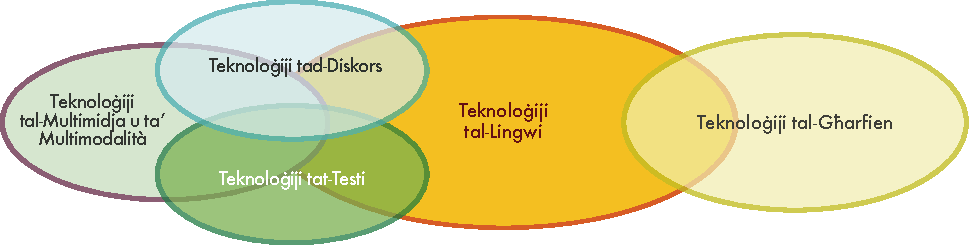
\includegraphics[width=\textwidth]{../_media/maltese/language_technologies}
  \caption{Sprachtechnologie im Kontext}
  \label{fig:ltincontext_de}
  \colorrule{grey3}{\textwidth}{1.5pt}
\end{figure*}

\subsection{Arkitetturi ta’ Applikazzjonijiet}

Applikazzjonijiet ta’ software tipiċi għall-ipproċessar tal-lingwa jikkonsistu f'diversi komponenti li jirriflettu aspetti differenti tal-lingwa u tal-kompitu li jkunu qed jimplimentaw. Ir-rappreżentazzjoni~\ref{fig:textprocessingarch_mt}  turi arkitettura ferm simplifikata li tista’ tinsab f’sistema ta’ pproċessar ta’ testi. L-ewwel tliet moduli jittrattaw l-istruttura u t-tifsira tat-test imdaħħal fis-sistema: 

\begin{figure*}[htb]
  \colorrule{grey3}{\textwidth}{1.5pt}
  \center
  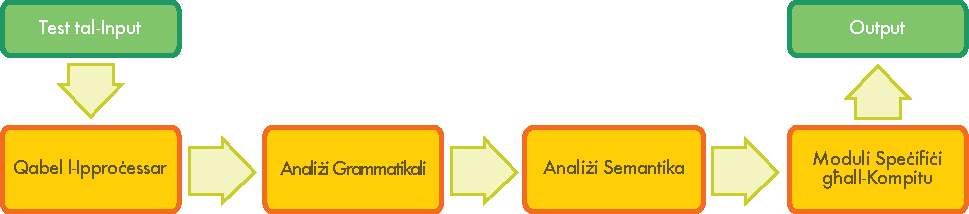
\includegraphics[width=\textwidth]{../_media/maltese/text_processing_app_architecture}
  \caption{Arkitettura tipika għall-ipproċessar ta' testi}
  \label{fig:textprocessingarch_mt}
  \colorrule{grey3}{\textwidth}{1.5pt}
\end{figure*}

\begin{enumerate}
\item Qabel l-ipproċessar: tindif tad-dejta, tneħħija tal-ifformattjar fejn hu xieraq, sejbien tal-lingwa mdaħħla fis-sistema, standardizzazjoni tar-rappreżentazzjoni ta’ simboli speċjali bħas-sing fil-Malti.
\item Analiżi grammatikali:  tiftix tal-verb u l-oġġetti tiegħu, il-modifikaturi, eċċ;  sejbien tal-istruttura tas-sentenza.
\item Analiżi semantika: tneħħja tal-ambigwità (Liema tifsira ta’ “bank” hija t-tajba f’kuntest partikolari?), soluzzjoni ta’ anafori u espressjonijiet ta' referenza bħal “hi”, “il-karozza”, eċċ; rappreżentazzjoni tat-tifsira tas-sentenza b’mod li tinqara minn magna.
\end{enumerate}

Moduli ta’ kompiti speċifiċi mbagħad iwettqu ħafna operazzjonijiet differenti bħal sommarju awtomatiku ta’ test imdaħħal fis-sistema, tfittxija ta’ bażi ta' dejta u ħafna oħrajn. Hawn taħt, se nagħtu eżempji ta’ \textbf{oqsma ewlenin ta’ applikazzjoni} u niġbdu l-attenzjoni għal xi wħud mill-moduli ta’ arkitetturi differenti f'kull sezzjoni. Għal darb’oħra, l-arkitetturi huma simplifikati ferm u idealizzati, sabiex iservu biex wieħed jispjega l-kumplessità tal-applikazzjonijiet tat-teknoloġija lingwistika b'mod ġenerali li jinftiehem.

Wara l-introduzzjoni tal-oqsma ewlenin ta’ applikazzjoni, se nagħtu ħarsa ġenerali fil-qosor lejn is-sitwazzjoni fir-riċerka u l-edukazzjoni tat-TL, u nikkonkludu b’deskrizzjoni ta’ programmi ta’ ffinanzjar (tal-passat). Fl-aħħar ta’ din it-taqsima, se nippreżentaw stima esperta dwar is-sitwazzjoni fir-rigward ta’ għodod prinċipali u riżorsi tat-TL f’numru ta’ dimensjonijiet bħal disponibbiltà, maturità, jew kwalità. It-tabella~\ref{fig:lrlttable_mt} fuq paġna~\pageref{fig:lrlttable_mt} tagħti ħarsa ġenerali tajba lejn is-sitwazzjoni tat-TL għall-Malti.

\subsection{Oqsma ewlenin ta’ applikazzjoni} 

\subsubsection{L-Iċċekkjar tal-lingwa}

Kull min juża għodda ta’ pproċessar tal-kliem bħal Microsoft Word iltaqa’ ma’ komponent li jiċċekkja l-ortografija, jindika żbalji ortografiċi u jipproponi korrezzjonijiet. 40 sena wara l-ewwel programm ta’ korrezzjoni tal-ortografija minn Ralph Gorin, ċekkjaturi lingwistiċi llum ma jqabblux biss il-lista ta’ kliem estratta ma’ dizzjunarju ta’ kliem spellut b’mod korrett, iżda saru dejjem aktar sofistikati. Minbarra l-algoritmi li jiddependu fuq il-lingwa għall-immaniġġjar tal-\underline{morfoloġija} (eż. formazzjoni tal-plural), xi wħud issa huma kapaċi jagħrfu żbalji marbuta ma’ sintassi, bħal verb nieqes jew verb li ma jaqbilx mas-suġġett tiegħu fil-persuna u n-numru, eż. f’ \emph{`She *write a letter.’} Madankollu, iċ-ċekkjaturi l-aktar disponibbli (inkluż Microsoft Word) ma jsibu l-ebda żbalji fl-ewwel vers ta’ poeżija \cite{zar1} %minn Jerrold H. Zar (1992) 
li tidher hawn taħt:

\begin{quote}
  I have a spelling checker,\\
  It came with my PC.\\
  It plane lee marks four my revue\\
  Miss steaks aye can knot sea.
\end{quote}

Għall-immaniġġjar ta’ dan it-tip ta’ żbalji, l-analiżi tal-\underline{kuntest} huwa meħtieġ f'ħafna każijiet, eż. sabiex jiġi deċiż f'liema pożizzjoni l-għ siekta għandha tinkiteb f’verb Malti, bħal f’dan l-eżempju:

\begin{enumerate} %[(a)]
\item \textit{... in-negozjati li kien għamel il-Gvern ...}
\item \textit{Pawlu, agħmel l-eżamijiet!}
\item *\textit{... in-negozjati li kien agħmel il-Gvern ...}
\end{enumerate}

Iż-żewġ verbi għamel  u agħmel jiġu ppronunzjati [ɐː.mɛl].

Dan jew jeħtieġ il-formulazzjoni ta’ regoli tal-\underline{grammatika} li jkunu  speċifiċi, jiġifieri livell għoli ta’ kompetenza u xogħol manwali, jew l-użu tal-hekk imsejjaħ \underline{mudell lingwistiku} tal-istatistika. Mudelli bħal dawn jikkalkulaw il-probabbiltà ta’ kelma partikolari li tidher f’ambjent speċifiku (jiġifieri, il-kliem ta’ qabel u ta’ wara). Pereżempju, kien għamel hija sekwenza ta’ kliem ħafna aktar probabbli milli kien agħmel. Mudell lingwistiku tal-statistika jista’ jitnissel awtomatikament  minn ammont kbir ta’ dejta lingwistika (xierqa) (jiġifieri \underline{korpus}). Sa issa, dawn il-metodi ġew l-aktar żviluppati u evalwati fuq dejta lingwistika bl-Ingliż. Madankollu, dawn mhux neċessarjament jittrasferixxu sew għal-lingwi li jkollhom inflessjoni għolja bħall-Malti, fejn tip ta’ kelma partikolari, bħal verb, tista’ tagħti numru kbir ta’ forom ortografiċi.

L-użu ta’ Ċekkjaturi Lingwistiċi mhuwiex limitat għal għodod ta’ pproċessar tal-kliem, iżda jiġi wkoll applikat f’sistemi ta’ appoġġ għal min jikteb. L-ammont ta’ dokumentazzjoni teknika li jakkumpanja l-għadd dejjem jikber ta’ prodotti tekniċi, żdied b’mod mgħaġġel matul l-aħħar deċennji. Minħabba l-biża’ tal-ilmenti tal-klijenti dwar l-użu ħażin u talbiet għal danni li jirriżultaw minn istruzzjonijiet ħżiena jew mifhuma ħażin, il-kumpaniji bdew jiffokaw dejjem aktar fuq il-kwalità tad-dokumentazzjoni teknika, fl-istess ħin jimmiraw għas-suq internazzjonali. Avvanzi fl-ipproċessar lingwistiku naturali wasslu għall-iżvilupp ta’ software ta’ appoġġ għal min jikteb, li jgħin lill-kittieb ta’ dokumentazzjoni teknika sabiex juża vokabolarju u strutturi ta’ sentenzi konsistenti ma’ ċerti regoli u restrizzjonijiet (korporattivi) tat-terminoloġija. 

\begin{figure*}[htb]
  \colorrule{grey3}{\textwidth}{1.5pt}
  \center
  
\includegraphics[width=\textwidth]{../_media/maltese/language_checking}
  \caption{Verifika tal-Lingwa (xellug: ibbażat fuq ir-regoli, lemin: statistika)}
  \label{fig:langcheckingaarch_mt}
  \colorrule{grey3}{\textwidth}{1.5pt}
\end{figure*}

Bħal lingwi oħra, mezz biex jiddetermina jekk sensiela partikolari hijiex kelma valida mhux kundizzjoni suffiċjenti għal sejbien ta’ żbalji ortografiċi, iżda huwa kundizzjoni neċessarja. S’issa, għalkemm saru diversi tentattivi, l-ebda mezz bħal dan ma jeżisti għall-Malti.

Wieħed minn tal-ewwel kien ta’ \cite{Mangion:1999} li juża forom rudimentali ta’ analiżi morfoloġiċi bbażati fuq regoli. Kelma kienet essenzjalment ikkunsidrata valida jekk tistax tkun derivata permezz ta' zokk misjub f’dizzjunarju. Il-problema b’ dan il-metodu huwa li jeħtieġ lista kompluta ta’ kull zokk, u naturalment, ir-regoli għandhom ikunu preċiżi ħafna. Ir-riżultati kienu kemxejn limitati mil-lista ta’ zkuk, li ma kinitx kompluta, u n-natura imperfetta tar-regoli.

Metodu ieħor ħares lejn l-istatistiċi għal soluzzjoni. L-idea intuwittiva hija li għal lingwa partikolari, ċerti sekwenzi ta’ karattri huma improbabbli ħafna. Bl-Ingliż, pereżempju, qatt ma nsibu s-sekwenza \emph{kk}, għalhekk jekk isseħħ taħt l-istess sekwenza f’kelma miktuba, nistgħu nbassru, bi grad għoli ta’ kunfidenza, li l-kelma mhijiex valida. B’mod aktar ġenerali, nistgħu nikkalkulaw il-probabbiltà ta’ xi sekwenza bħala funzjoni tal-probabbiltajiet tas-sekwenzi ta’ taħtha kollha, bl-adozzjoni tal-prinċipju li sabiex il-kelma tiġi kkunsidrata valida, il-probabbiltà trid taqbeż ċertu limitu.

Ċekkjatur ortografiku statistiku li jagħmel użu minn prinċipju bħal dan kien żviluppat minn \cite{Mizzi:2001}. Dan ma kienx jeħtieġ dizzjunarju, iżda minflok kien ibbażat fuq id-distribuzzjoni ta’ n-grammi ta' karattri misjuba f’korpus ta’ gazzetta. Deher ċar li biex dan il-metodu jirnexxi kien jeħtieġ (i) mudell lingwistiku aktar preċiż li jirrikjedi aktar dejta lingwistika minn dik disponibbli dak iż-żmien, u (ii) li l-probabbiltà tas-sekwenza waħedha ma kinitx biżżejjed sabiex kelma ortografika tiġi kklassifikata bħala żball. Kif issuġġerit hawn fuq, informazzjoni oħra hija meħtieġa, bħal kategorija tal-kliem mill-kuntest tal-madwar.

Tentattivi oħra biex jiġi żviluppat ċekkjatur ortografiku għall-Malti jinkludu ċekkjatur fuq l-internet li ġie żviluppat minn Ramon Casha tal-Linux User Group\cite{Linux-spellcheck1}. Dan huwa bbażat fuq lista ta’ kliem b’madwar miljun tip ta’ kelma oriġinarjament miġbura minn korpus li jvarja, u sussegwentement estiż permezz ta’ regoli differenti għall-immaniġġjar ta’ inflessjonijiet. L-eżattezza tiegħu ma ġietx stabbilita uffiċjalment. Microsoft ukoll kienu qed jaħdmu fuq ċekkjatur ortografiku biex jinkluduh mal-pakkett ta’ interface tagħhom għal-lingwa Maltija għalkemm mhux magħruf meta dan se jiġi rilaxxat.

L-użu ta’ ċekkjatur lingwistiku mhuwiex limitat għal għodod ta’  pproċessar tal-kliem. Oqsma ta’ applikazzjoni oħra jinkludu \textbf{appoġġ għal min jikteb}, pereżempju biex jgħin lill-kittieb ta’ dokumentazzjoni teknika juża vokabolarju tekniku b’mod konsistenti, u l-qasam tat-\textbf{tagħlim tal-lingwi assistit mill-kompjuter}. L-iċċekkjar tal-lingwa jiġi wkoll applikat biex jiġu kkoreġuti awtomatikament mistoqsijiet mibgħuta lil magni ta’ tiftix, eż. suġġerimenti tat-tip ``Ridt tfisser ...'' lil Google. 

Barra minn CD ta’ dizzjunarju interattiv bl-istampi \cite{Sciriha:1997}, sal-lum l-ebda applikazzjoni bħal din ma ġiet żviluppata għall-Malti.

  
\subsubsection{L-Interazzjoni tat-taħdit }

L-interazzjoni tat-taħdit hija l-bażi għall-ħolqien ta’ interfaces li jippermettu lill-utent biex jinteraġixxi ma’ magni billi juża l-lingwa mitkellma aktar milli, pereżempju, stampa grafika, tastiera, u mouse. Illum, l-interfaces għall-vuċi (VUIs) huma normalment użati għal offerti ta’ servizzi ta’ awtomatizzazzjoni parzjali jew kompluti pprovduti mill-kumpaniji lill-klijenti tagħhom, l-impjegati jew l-imsieħba permezz tat-telefon. Dominji ta’ negozju li jiddependu ħafna fuq VUIs huma l-banek, il-loġistika, it-trasport pubbliku, u t-telekomunikazzjonijiet. Użi oħra tat-Teknoloġija għall-Interazzjoni tat-Taħdit huma interfaces għal apparat partikolari, eż. sistemi ta’ navigazzjoni fil-karozza, u l-użu tal-lingwa mitkellma bħala alternattiva għall-modalitajiet ta’ input/output ta’ interfaces grafiċi għall-utent, eż. fl-ismartphones.

\boxtext{Sprachliche Interaktion ist die Grundlage für die Schaffung von Schnittstellen, über die ein Nutzer mittels gesprochener Sprache interagieren kann statt über eine grafische Anzeige, Tastatur und Maus.}

\begin{figure*}[htb]
  \colorrule{grey3}{\textwidth}{1.5pt}
  \center 
  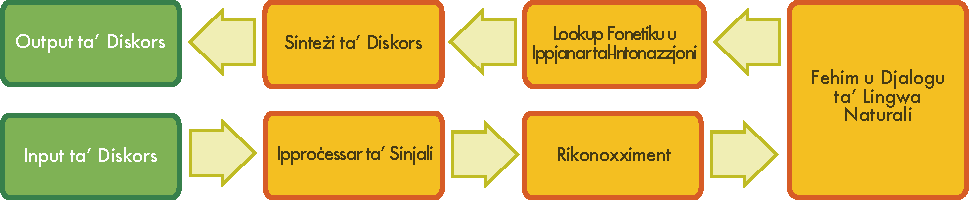
\includegraphics[width=\textwidth]{../_media/maltese/simple_speech-based_dialogue_architecture}
  \caption{Sistema tal-interazzjoni tat-taħdit}
  \label{fig:dialoguearch_mt}
  \colorrule{grey3}{\textwidth}{1.5pt}
\end{figure*}

Fil-qalba tagħha, l-Interazzjoni tat-Taħdit tinkludi l-erba’ teknoloġiji differenti li ġejjin:

\begin{enumerate}
\item L-Identifikazzjoni awtomatika tat-taħdit (ASR) hija responsabbli biex tiddetermina liema kliem kien attwalment mitkellem f’sekwenza partikolari ta’ ħsejjes imlissna minn utent.
\item L-analiżi sintattika u l-interpretazzjoni semantika janalizzaw l-istruttura sintattika tat-tlissin tal-utent u jinterpretaw tal-aħħar skont l-għan tas-sistema rispettiva.
\item Il-ġestjoni tad-djalogu hija meħtieġa sabiex jiġi determinata ma’ liema parti tas-sistema l-utent jinteraġixxi, liema azzjoni għandha tittieħed skont l-input tal-utent u l-funzjonalità tas-sistema.
\item It-teknoloġija tas-sinteżi tat-taħdit (Text-to-Speech, TTS) hija użata biex tittrasforma l-kliem ta’ dik l-espressjoni fi ħsejjes li jkunu prodotti għall-utent. 
\end{enumerate}

Waħda mill-isfidi ewlenin hija li jkollok sistema ASR li tidentifika  l-kliem imlissen minn utent bl-aktar mod preċiż possibbli. Dan jeħtieġ jew restrizzjoni tal-firxa ta’ espressjonijiet possibbli tal-utent għal sett limitat ta’ kliem ewlieni, inkella l-ħolqien manwali ta’ \underline{mudelli lingwistiċi} li jkopru firxa kbira ta’ espressjonijiet ta’ lingwa naturali tal-utent. Filwaqt li tal-ewwel jirriżulta f’użu pjuttost riġidu u inflessibbli ta’ VUI u li  possibilment jikkawża aċċettazzjoni baxxa mill-utenti, il-ħolqien, l-irfinar u l-manutenzjoni tal-mudelli lingwistiċi jistgħu jżidu l-ispejjeż b’mod sinifikanti. Madankollu, il-VUIs li jużaw mudelli lingwistiċi u fil-bidu jippermettu lill-utent biex jesprimi l-intenzjoni tiegħu b’mod flessibbli – evokati, pereżempju, minn tislima bħal ‘Kif nista’ ngħinek’ – għandha kemm rata ogħla ta’ awtomazzjoni, kif ukoll aktar aċċettazzjoni mill-utenti u għalhekk jistgħu jitqiesu bħala vantaġġużi fuq il-metodu ta’ djalogu dirett u anqas flessibbli. Għall-parti tal-output tal-VUI, il-kumpaniji għandhom tendenza li jużaw ħafna espressjonijiet irrekordjati minn qabel ta’ kelliema professjonali – idealment korporattivi. Għal espressjonijiet statiċi, li fihom il-kliem ma jiddependix fuq il-kuntesti partikolari tal-użu jew id-dejta personali ta’ utent partikolari, dan iwassal għal esperjenza rikka tal-utent. Madankollu, aktar ma l-espressjoni jkollha tikkunsidra kontenut dinamiku, aktar l-esperjenza tal-utent tista’ tbati aktar minn prosodija fqira li tirriżulta minn files audio individwali marbutin ma’ xulxin. B'kuntrast ma’ dan, is-sistemi TTS tal-lum, jagħtu xhieda li huma superjuri, għalkemm jistgħu jintużaw aħjar, fir-rigward tan-naturalezza prosodika ta’ espressjonijiet dinamiċi.

Rigward is-suq tat-teknoloġija għall-Interazzjoni tat-Taħdit, l-aħħar għaxar snin għaddew minn standardizzazzjoni qawwija tal-interfaces bejn il-komponenti ta’ teknoloġiji differenti, kif ukoll bi standards għal ħolqien ta’ prodotti ta’ software partikolari għal ċerta applikazzjoni. F’dawn l-aħħar għaxar snin kien hemm ukoll konsolidazzjoni soda tas-suq, partikolarment fil-qasam tal-ASR u t-TTS. Hawnhekk, is-swieq nazzjonali fil-pajjiżi tal-G20 – jiġifieri pajjiżi ekonomikament b'saħħithom b’popolazzjoni konsiderevoli - huma dominati minn anqas minn 5 parteċipanti dinjija, b’Nuance u Loquendo dawk l-aktar prominenti fl-Ewropa.

Ħafna mill-iżvilupp tat-teknoloġija tat-taħdit f'Malta kkonċentra fuq 'mit-test għat-taħdit' (TTS). Xi xogħol pijunier fil-bidu kien imwettaq minn \cite{Micallef:1997} u dan kien segwit minn numru ta’ teżijiet f’livell ta’ Masters \cite{Farrugia:2005}. Xi xogħol fuq sistema TTS ibbażata fuq il-web beda minn \cite{Buhagiar-Micallef:2008}.
Żvilupp sinifikanti fis-sinteżi tat-taħdit għall-Malti kien il-kisba ta’ offerta mingħand il-gvern għall-iżvilupp ta’ sintetizzatur tat-taħdit mill-kumpanija lokali Crimson Wing Ltd. Malta. Dan ix-xogħol huwa parzjalment iffinanzjat mill-Fond Ewropew għall-Iżvilupp Reġjonali u kkummissjonat mill-Fondazzjoni għall-Aċċessibilità għat-Teknoloġija tal-Informazzjoni (FITA). Il-prototip se jkun konformi ma’ SAPI u se jinkludi tliet vuċijiet (tal-irġiel, tan-nisa, u tat-tfal). Skont preżentazzjoni riċenti \cite{Borg-et-al:2011} ix-xogħol qed javvanza sew u prototip, mistenni fl-2012, se jkun disponibbli biex jitniżżel mingħajr ħlas.

Ix-xogħol fuq l-idenifikazzjoni tat-taħdit huwa anqas avvanzat. Prototip biex jidentifika n-numri nħoloq minn \cite{Calleja:2004} f’dominji sempliċi. Fir-rigward tat-taħdit, il-problema fundamentali tibqa’ nuqqas ta’ dejta annotata b’mod xieraq minħabba li dan jeħtieġ sforz manwali sinifikanti. Xi tentattivi ta’ dħul awtomatiku saru minn \cite{Psaila:2008}. Il-ħolqien ta’ korpus u qafas deskrittiv għall-istudju tal-intonazzjoni Maltija bdiet mill-Istitut tal-Lingwistika u twettqet minn Vella u Farrugia \cite{Vella-Farrugia:2006}. Huwa mistenni li l-korpus li qed jiġi żviluppat minn Crimson Wing se jkun disponibbli għar-riċerka.

Ħarsa lil hinn mill-istat tat-teknoloġija tal-lum, turi li se jkun hemm bidliet sinifikanti minħabba l-firxa ta’ smartphones bħala pjattaforma ġdida għall-ġestjoni ta’ relazzjonijiet mal-klijenti – minbarra t-telefon, l-internet u mezzi għall-posta elettronika. Din it-tendenza se taffettwa wkoll l-użu tat-teknoloġija għall-Interazzjoni tat-Taħdit. Minn naħa, id-domanda għal telefonija bbażata fuq VUIs se tonqos, fuq medda ta' tul ta’ żmien. Min-naħa l-oħra, l-użu tal-lingwa mitkellma bħala modalità ta’ input faċli għall-utent għall-ismartphones se jikseb importanza sinifikanti. Din it-tendenza hija appoġġjata minn titjib osservabbli tal-eżattezza tal-identifikazzjoni tad-diskors li hija indipendenti mill-kelliem għal dettatura ta’ taħdit li diġà hija offruta bħala servizzi ċentralizzati għall-utenti tal-ismartphone. B’din l-‘esternalizzazzjoni’ tal-kompitu ta’ identifikazzjoni tal-infrastruttura tal-applikazzjonijiet, l-użu ta’ applikazzjoni speċifika ta’ teknoloġiji ewlenin lingwistiċi għandha tikber fl-importanza meta mqabbla mas-sitwazzjoni preżenti.


\subsubsection{Traduzzjoni awtomatika}

L-idea tal-użu ta’ kompjuters diġitali għat-traduzzjoni ta’ lingwi naturali bdiet fl-1946 minn A. D. Booth u kienet segwita minn fondi sostanzjali għar-riċerka f'dan il-qasam fil-ħamsinijiet u ssoktat mill-ġdid fit-tmeninijiet. Madankollu, it-\underline{Traduzzjoni Awtomatika} (TA) tibqa’ tonqos li tissodisfa l-aspettativi għolja li ħolqot fis-snin bikrin tagħha.

\boxtext{Fil-livell bażiku tagħha, TA sempliċiment tissostitwixxi l-kliem ta' lingwa naturali waħda b'ta' oħra.}

Fil-livell bażiku tagħha, TA sempliċiment tissostitwixxi l-kliem ta' lingwa naturali waħda b'ta' oħra. Dan jista’ jkun utli f'dominji ta' suġġetti b’lingwa ristretta u konvenzjonali ħafna, pereżempju, rapporti tat-temp. Madankollu, għal traduzzjoni tajba ta’ testi anqas standardizzati, unitajiet ta’ testi akbar (frażijiet, sentenzi, jew anki siltiet sħaħ) jeħtieġ li jkunu mqabbla mal-eqreb kontropartijiet tagħhom fil-lingwa fil-mira. Id-diffikultà prinċipali hawnhekk tinsab fil-fatt li l-lingwa umana hija ambigwa, u toħloq  sfidi fuq livelli multipli, eż. \underline{tneħħija ta’ ambigwità mis-sens tal-kelma} fuq livell lessikali (`Jaguar' tista’ tfisser karozza jew annimal) jew it-twaħħil ta’ frażijiet prepożizzjonali fuq livell sintattiku bħal fl-eżempji li ġejjin:

\begin{enumerate}%[(a)]
\item \emph{Il-Kuntistabbli osserva lir-raġel bit-teleskopju.}
\item \emph{Il-Kuntistabbli osserva lir-raġel bir-rivolver.}
\end{enumerate}

Mod wieħed kif wieħed jitratta l-kompitu huwa bbażat fuq regoli lingwistiċi. Għat-traduzzjonijiet bejn lingwi marbutin flimkien mill-qrib, traduzzjoni diretta tista’ tkun possibbli f'każijiet bħall-eżempju t’hawn fuq. Iżda sistemi bbażati fuq regoli (jew immexxija minn għarfien) ta’ spiss janalizzaw it-test imdaħħal fis-sistema u joħolqu rappreżentazzjoni intermedjarja u simbolika, li minnhom it-test fil-lingwa fil-mira jiġi ġġenerat. Is-suċċess ta’ dawn il-metodi jiddipendi ħafna fuq id-disponibbiltà ta’ \underline{dizzjunarji} estensivi b’ informazzjoni morfoloġika, sintattika, u semantika, u settijiet kbar ta’ regoli tal-\underline{grammatika} mfassla bir-reqqa minn lingwista tas-sengħa.

\begin{figure*}[htb]
  \colorrule{grey3}{\textwidth}{1.5pt}
  \center
  
\includegraphics[width=\textwidth]{../_media/maltese/machine_translation}
  \caption{Traduzzjoni awtomatika (statistika; ibbażata fuq regoli)}
  \label{fig:mtarch_mt}
  \colorrule{grey3}{\textwidth}{1.5pt}
\end{figure*}

Lejn it-tmiem tat-tmeninijiet, kif l-enerġija kompjutazzjonali żdiedet u saret anqas għalja, kien hemm aktar interess fil-mudelli statistiċi għat-TA. Il-parametri ta’ dawn il-mudelli statistiċi jittieħdu mill-analiżi ta’ \underline{korpora} ta’ testijiet bilingwi, bħalma hu l-korpus parallel tal-Europarl, li fih il-proċedimenti tal-Parlament Ewropew fi 11-il lingwa Ewropea. B’dejta suffiċjenti, TA statistika jaħdem tajjeb biżżejjed li jikseb tifsira approssimattiva għal test ta’ lingwa barranija. Madankollu, bid-differenza ta’ sistemi mmexxija mill-għarfien, it-TA statistika (jew immexxija minn dejta) spiss tiġġenera produzzjoni mhux grammatikali. Min-naħa l-oħra, minbarra l-vantaġġ li anqas sforz uman huwa meħtieġ għall-kitba grammatikali, TA mmexxija minn dejta tista’ wkoll tkopri partikolaritajiet tal-lingwa li jintilfu f’sistemi mmexxija minn għarfien, pereżempju espressjonijiet idjomatiċi.

Minħabba li l-punti tajbin u dgħajfin tat-TA mmexxija minn għarfien u dejta huma kumplimentari, ir-riċerkaturi llum unanimament jimmiraw għal metodi ibridi li jgħaqqdu l-metodoloġiji tat-tnejn li huma. Dan jista’ jsir b’modi diversi. Wieħed jinkludi l-użu ta’ kemm sistemi mmexxija minn għarfien kif ukoll dejta u jkollu modulu ta’ għażla li jiddeċiedi dwar l-aħjar output għal kull sentenza. Madankollu, għal sentenzi itwal, l-ebda riżultat mhu se jkun perfett. Soluzzjoni aħjar hija li tgħaqqad l-aħjar partijiet ta’ kull sentenza minn outputs multipli, li jistgħu jkunu pjuttost kumplessi, minħabba li partijiet korrispondenti ta’ alternattivi multipli mhux dejjem huma ovvji u jridu jkunu allinjati.

\boxtext{Il-kwalità tas-sistemi tat-TA għall-Malti hija meqjusa li għad għandha potenzjal kbir ta’ titjib.} 

F’Malta l-ħidma mwettqa fit-Traduzzjoni Awtomatika kienet ristretta għal ftit teżijiet tal-grad ta’ Baċellerat u Masters. Sistema ta’ trasferiment ibbażata fuq l-LFG kienet żviluppata għall-Ingliż/Malti minn \cite{Farrugia:2000} u kienet tittraduċi b’suċċess it-tbassir tat-temp. Aktar tard J. Bajada \cite{Bajada:2004, Bajada:2009} ħadem fuq TA statistika (SMT) bl-enfasi fuq tekniki għall-produzzjoni ta’ mudelli lingwistiċi u tat-traduzzjoni. Ix-xogħol preċedenti kien jikkonċerna mudelli bbażati fuq kliem, filwaqt li tal-aħħar żviluppa tekniki għal ġbir ta’ dejta bilingwali ta’ frażijiet minn korpus limitat.

Bħal f'bosta oqsma oħra, il-problema bażika hija n-nuqqas ta’ kwantitajiet kbar ta’ dejta bilingwali annotata b’mod xieraq. Minħabba din ir-raġuni, forsi, is-sistema bil-punt ta’ referenza biex jiġu ġġudikati avvanzi tibqa’ Google Translate.

Il-kwalità tas-sistemi tat-TA hija meqjusa li għad għandha potenzjal kbir ta’ titjib. L-isfidi jinkludu l-adattabilità tar-riżorsi lingwistiċi għal dominju ta’ suġġett partikolari jew qasam tal-utent u l-integrazzjoni tax-xogħol għaddej eżistenti b’bażijiet ta’ termini u memorji tat-traduzzjoni. Barra minn hekk, ħafna mis-sistemi kurrenti huma bbażati fuq l-Ingliż u jappoġġjaw lil ftit biss mil-lingwi minn u għall-Ġermaniż, li jwassal għal tensjonijiet fix-xogħol għaddej totali tat-traduzzjoni, u eż. jisforza utenti tat-TA biex jitgħallmu għodod ta’ kodiċi ta’ lessiku differenti għal sistemi differenti.

Kampanji ta’ evalwazzjoni jippermettu tqabbil tal-kwalità tas-sistemi tat-TA, il-metodi diversi u l-istatus ta’ sistemi TA għal-lingwi differenti. It-tabella~\ref{fig:euromatrix_mt}, ippreżentata fi ħdan il-proġett Euromatrix+ tal-KE, turi l-prestazzjonijiet par par miksuba għal 22 lingwa uffiċjali (il-Gaelic Irlandiż huwa nieqes) f'termini ta’ punteġġ BLEU \cite{bleu1}. Aktar ma jkun għoli l-punteġġ, aktar tkun tajba t-traduzzjoni. Traduttur uman iġib madwar 80 \cite{bleu1}.

L-aħjar riżultati (murija bl-aħdar u l-blu) nkisbu minn lingwi li jibbenefikaw minn sforzi konsiderevoli ta’ riċerka, fi ħdan programmi kkoordinati, u mill-eżistenza ta’ korpora paralleli u numerużi  (eż. Ingliż, Franċiż, Olandiż, Spanjol, Ġermaniż), l-agħar (bl-aħmar) minn lingwi li ma bbenefikawx minn sforzi simili, jew li huma differenti ħafna minn lingwi oħra (eż. Ungeriż, Malti, Finlandiż).

\begin{figure*}[htbp]
  \centering
  \setlength{\tabcolsep}{0.17em}
  \small
  \begin{tabular}{>{\columncolor{corange1}}cccccccccccccccccccccccc}
    & \multicolumn{22}{>{\columncolor{corange1}}c}{Lingwa tal-mira -- \textcolor{grey1}{Target language}}\\\addlinespace[{-.009cm}]
    \rowcolor{corange1}  & EN & BG & DE & CS & DA & EL & ES & ET & FI & FR & HU & IT & LT & LV & MT & NL & PL & PT & RO & SK & SL & SV\\
    EN & -- & \textcolor{blue}{40.5} & \textcolor{blue}{46.8} & \textcolor{green2}{52.6} & \textcolor{green2}{50.0} & \textcolor{blue}{41.0} & \textcolor{green2}{55.2} & \textcolor{purple}{34.8} & \textcolor{purple}{38.6} & \textcolor{green2}{50.1} & \textcolor{purple}{37.2} & \textcolor{green2}{50.4} & \textcolor{purple}{39.6} & \textcolor{blue}{43.4} & \textcolor{purple}{39.8} & \textcolor{green2}{52.3} & \textcolor{blue}{49.2} & \textcolor{green2}{55.0} & \textcolor{blue}{49.0} & \textcolor{blue}{44.7} & \textcolor{green2}{50.7} & \textcolor{green2}{52.0}\\
    BG & \textcolor{green}{61.3} & -- & \textcolor{purple}{38.7} & \textcolor{purple}{39.4} & \textcolor{purple}{39.6} & \textcolor{purple}{34.5} & \textcolor{blue}{46.9} & \textcolor{red3}{25.5} & \textcolor{red3}{26.7} & \textcolor{blue}{42.4} & \textcolor{red3}{22.0} & \textcolor{blue}{43.5} & \textcolor{red3}{29.3} & \textcolor{red3}{29.1} & \textcolor{red3}{25.9} & \textcolor{blue}{44.9} & \textcolor{purple}{35.1} & \textcolor{blue}{45.9} & \textcolor{purple}{36.8} & \textcolor{purple}{34.1} & \textcolor{purple}{34.1} & \textcolor{purple}{39.9}\\
    DE & \textcolor{green2}{53.6} & \textcolor{red3}{26.3} & -- & \textcolor{purple}{35.4} & \textcolor{blue}{43.1} & \textcolor{purple}{32.8} & \textcolor{blue}{47.1} & \textcolor{red3}{26.7} & \textcolor{red3}{29.5} & \textcolor{purple}{39.4} & \textcolor{red3}{27.6} & \textcolor{blue}{42.7} & \textcolor{red3}{27.6} & \textcolor{purple}{30.3} & \textcolor{red2}{19.8} & \textcolor{green2}{50.2} & \textcolor{purple}{30.2} & \textcolor{blue}{44.1} & \textcolor{purple}{30.7} & \textcolor{red3}{29.4} & \textcolor{purple}{31.4} & \textcolor{blue}{41.2}\\
    CS & \textcolor{green2}{58.4} & \textcolor{purple}{32.0} & \textcolor{blue}{42.6} & -- & \textcolor{blue}{43.6} & \textcolor{purple}{34.6} & \textcolor{blue}{48.9} & \textcolor{purple}{30.7} & \textcolor{purple}{30.5} & \textcolor{blue}{41.6} & \textcolor{red3}{27.4} & \textcolor{blue}{44.3} & \textcolor{purple}{34.5} & \textcolor{purple}{35.8} & \textcolor{red3}{26.3} & \textcolor{blue}{46.5} & \textcolor{purple}{39.2} & \textcolor{blue}{45.7} & \textcolor{purple}{36.5} & \textcolor{blue}{43.6} & \textcolor{blue}{41.3} & \textcolor{blue}{42.9}\\
    DA & \textcolor{green2}{57.6} & \textcolor{red3}{28.7} & \textcolor{blue}{44.1} & \textcolor{purple}{35.7} & -- & \textcolor{purple}{34.3} & \textcolor{blue}{47.5} & \textcolor{red3}{27.8} & \textcolor{purple}{31.6} & \textcolor{blue}{41.3} & \textcolor{red3}{24.2} & \textcolor{blue}{43.8} & \textcolor{red3}{29.7} & \textcolor{purple}{32.9} & \textcolor{red3}{21.1} & \textcolor{blue}{48.5} & \textcolor{purple}{34.3} & \textcolor{blue}{45.4} & \textcolor{purple}{33.9} & \textcolor{purple}{33.0} & \textcolor{purple}{36.2} & \textcolor{blue}{47.2}\\
    EL & \textcolor{green2}{59.5} & \textcolor{purple}{32.4} & \textcolor{blue}{43.1} & \textcolor{purple}{37.7} & \textcolor{blue}{44.5} & -- & \textcolor{green2}{54.0} & \textcolor{red3}{26.5} & \textcolor{red3}{29.0} & \textcolor{blue}{48.3} & \textcolor{red3}{23.7} & \textcolor{blue}{49.6} & \textcolor{red3}{29.0} & \textcolor{purple}{32.6} & \textcolor{red3}{23.8} & \textcolor{blue}{48.9} & \textcolor{purple}{34.2} & \textcolor{green2}{52.5} & \textcolor{purple}{37.2} & \textcolor{purple}{33.1} & \textcolor{purple}{36.3} & \textcolor{blue}{43.3}\\
    ES & \textcolor{green}{60.0} & \textcolor{purple}{31.1} & \textcolor{blue}{42.7} & \textcolor{purple}{37.5} & \textcolor{blue}{44.4} & \textcolor{purple}{39.4} & -- & \textcolor{red3}{25.4} & \textcolor{red3}{28.5} & \textcolor{green2}{51.3} & \textcolor{red3}{24.0} & \textcolor{green2}{51.7} & \textcolor{red3}{26.8} & \textcolor{purple}{30.5} & \textcolor{red3}{24.6} & \textcolor{blue}{48.8} & \textcolor{purple}{33.9} & \textcolor{green2}{57.3} & \textcolor{purple}{38.1} & \textcolor{purple}{31.7} & \textcolor{purple}{33.9} & \textcolor{blue}{43.7}\\
    ET & \textcolor{green2}{52.0} & \textcolor{red3}{24.6} & \textcolor{purple}{37.3} & \textcolor{purple}{35.2} & \textcolor{purple}{37.8} & \textcolor{red3}{28.2} & \textcolor{blue}{40.4} & -- & \textcolor{purple}{37.7} & \textcolor{purple}{33.4} & \textcolor{purple}{30.9} & \textcolor{purple}{37.0} & \textcolor{purple}{35.0} & \textcolor{purple}{36.9} & \textcolor{red3}{20.5} & \textcolor{blue}{41.3} & \textcolor{purple}{32.0} & \textcolor{purple}{37.8} & \textcolor{red3}{28.0} & \textcolor{purple}{30.6} & \textcolor{purple}{32.9} & \textcolor{purple}{37.3}\\
    FI & \textcolor{blue}{49.3} & \textcolor{red3}{23.2} & \textcolor{purple}{36.0} & \textcolor{purple}{32.0} & \textcolor{purple}{37.9} & \textcolor{red3}{27.2} & \textcolor{purple}{39.7} & \textcolor{purple}{34.9} & -- & \textcolor{red3}{29.5} & \textcolor{red3}{27.2} & \textcolor{purple}{36.6} & \textcolor{purple}{30.5} & \textcolor{purple}{32.5} & \textcolor{red2}{19.4} & \textcolor{blue}{40.6} & \textcolor{red3}{28.8} & \textcolor{purple}{37.5} & \textcolor{red3}{26.5} & \textcolor{red3}{27.3} & \textcolor{red3}{28.2} & \textcolor{purple}{37.6}\\
    FR & \textcolor{green}{64.0} & \textcolor{purple}{34.5} & \textcolor{blue}{45.1} & \textcolor{purple}{39.5} & \textcolor{blue}{47.4} & \textcolor{blue}{42.8} & \textcolor{green}{60.9} & \textcolor{red3}{26.7} & \textcolor{purple}{30.0} & -- & \textcolor{red3}{25.5} & \textcolor{green2}{56.1} & \textcolor{red3}{28.3} & \textcolor{purple}{31.9} & \textcolor{red3}{25.3} & \textcolor{green2}{51.6} & \textcolor{purple}{35.7} & \textcolor{green}{61.0} & \textcolor{blue}{43.8} & \textcolor{purple}{33.1} & \textcolor{purple}{35.6} & \textcolor{blue}{45.8}\\
    HU & \textcolor{blue}{48.0} & \textcolor{red3}{24.7} & \textcolor{purple}{34.3} & \textcolor{purple}{30.0} & \textcolor{purple}{33.0} & \textcolor{red3}{25.5} & \textcolor{purple}{34.1} & \textcolor{red3}{29.6} & \textcolor{red3}{29.4} & \textcolor{purple}{30.7} & -- & \textcolor{purple}{33.5} & \textcolor{red3}{29.6} & \textcolor{purple}{31.9} & \textcolor{red2}{18.1} & \textcolor{purple}{36.1} & \textcolor{red3}{29.8} & \textcolor{purple}{34.2} & \textcolor{red3}{25.7} & \textcolor{red3}{25.6} & \textcolor{red3}{28.2} & \textcolor{purple}{30.5}\\
    IT & \textcolor{green}{61.0} & \textcolor{purple}{32.1} & \textcolor{blue}{44.3} & \textcolor{purple}{38.9} & \textcolor{blue}{45.8} & \textcolor{blue}{40.6} & \textcolor{red3}{26.9} & \textcolor{red3}{25.0} & \textcolor{red3}{29.7} & \textcolor{green2}{52.7} & \textcolor{red3}{24.2} & -- & \textcolor{red3}{29.4} & \textcolor{purple}{32.6} & \textcolor{red3}{24.6} & \textcolor{green2}{50.5} & \textcolor{purple}{35.2} & \textcolor{green2}{56.5} & \textcolor{purple}{39.3} & \textcolor{purple}{32.5} & \textcolor{purple}{34.7} & \textcolor{blue}{44.3}\\
    LT & \textcolor{green2}{51.8} & \textcolor{red3}{27.6} & \textcolor{purple}{33.9} & \textcolor{purple}{37.0} & \textcolor{purple}{36.8} & \textcolor{red3}{26.5} & \textcolor{red3}{21.1} & \textcolor{purple}{34.2} & \textcolor{purple}{32.0} & \textcolor{purple}{34.4} & \textcolor{red3}{28.5} & \textcolor{purple}{36.8} & -- & \textcolor{blue}{40.1} & \textcolor{red3}{22.2} & \textcolor{purple}{38.1} & \textcolor{purple}{31.6} & \textcolor{purple}{31.6} & \textcolor{red3}{29.3} & \textcolor{purple}{31.8} & \textcolor{purple}{35.3} & \textcolor{purple}{35.3}\\
    LV & \textcolor{green2}{54.0} & \textcolor{red3}{29.1} & \textcolor{purple}{35.0} & \textcolor{purple}{37.8} & \textcolor{purple}{38.5} & \textcolor{red3}{29.7} & \textcolor{red2}{8.0} & \textcolor{purple}{34.2} & \textcolor{purple}{32.4} & \textcolor{purple}{35.6} & \textcolor{red3}{29.3} & \textcolor{purple}{38.9} & \textcolor{purple}{38.4} & -- & \textcolor{red3}{23.3} & \textcolor{blue}{41.5} & \textcolor{purple}{34.4} & \textcolor{purple}{39.6} & \textcolor{purple}{31.0} & \textcolor{purple}{33.3} & \textcolor{purple}{37.1} & \textcolor{purple}{38.0}\\
    MT & \textcolor{green}{72.1} & \textcolor{purple}{32.2} & \textcolor{purple}{37.2} & \textcolor{purple}{37.9} & \textcolor{purple}{38.9} & \textcolor{purple}{33.7} & \textcolor{blue}{48.7} & \textcolor{red3}{26.9} & \textcolor{red3}{25.8} & \textcolor{blue}{42.4} & \textcolor{red3}{22.4} & \textcolor{blue}{43.7} & \textcolor{purple}{30.2} & \textcolor{purple}{33.2} & -- & \textcolor{blue}{44.0} & \textcolor{purple}{37.1} & \textcolor{blue}{45.9} & \textcolor{purple}{38.9} & \textcolor{purple}{35.8} & \textcolor{blue}{40.0} & \textcolor{blue}{41.6}\\
    NL & \textcolor{green2}{56.9} & \textcolor{red3}{29.3} & \textcolor{blue}{46.9} & \textcolor{purple}{37.0} & \textcolor{blue}{45.4} & \textcolor{purple}{35.3} & \textcolor{blue}{49.7} & \textcolor{red3}{27.5} & \textcolor{red3}{29.8} & \textcolor{blue}{43.4} & \textcolor{red3}{25.3} & \textcolor{blue}{44.5} & \textcolor{red3}{28.6} & \textcolor{purple}{31.7} & \textcolor{red3}{22.0} & -- & \textcolor{purple}{32.0} & \textcolor{blue}{47.7} & \textcolor{purple}{33.0} & \textcolor{purple}{30.1} & \textcolor{purple}{34.6} & \textcolor{blue}{43.6}\\
    PL & \textcolor{green}{60.8} & \textcolor{purple}{31.5} & \textcolor{blue}{40.2} & \textcolor{blue}{44.2} & \textcolor{blue}{42.1} & \textcolor{purple}{34.2} & \textcolor{blue}{46.2} & \textcolor{red3}{29.2} & \textcolor{red3}{29.0} & \textcolor{blue}{40.0} & \textcolor{red3}{24.5} & \textcolor{blue}{43.2} & \textcolor{purple}{33.2} & \textcolor{purple}{35.6} & \textcolor{red3}{27.9} & \textcolor{blue}{44.8} & -- & \textcolor{blue}{44.1} & \textcolor{purple}{38.2} & \textcolor{purple}{38.2} & \textcolor{purple}{39.8} & \textcolor{blue}{42.1}\\
    PT & \textcolor{green}{60.7} & \textcolor{purple}{31.4} & \textcolor{blue}{42.9} & \textcolor{purple}{38.4} & \textcolor{blue}{42.8} & \textcolor{blue}{40.2} & \textcolor{green}{60.7} & \textcolor{red3}{26.4} & \textcolor{red3}{29.2} & \textcolor{green2}{53.2} & \textcolor{red3}{23.8} & \textcolor{green2}{52.8} & \textcolor{red3}{28.0} & \textcolor{purple}{31.5} & \textcolor{red3}{24.8} & \textcolor{blue}{49.3} & \textcolor{purple}{34.5} & -- & \textcolor{purple}{39.4} & \textcolor{purple}{32.1} & \textcolor{purple}{34.4} & \textcolor{blue}{43.9}\\
    RO & \textcolor{green}{60.8} & \textcolor{purple}{33.1} & \textcolor{purple}{38.5} & \textcolor{purple}{37.8} & \textcolor{blue}{40.3} & \textcolor{purple}{35.6} & \textcolor{green2}{50.4} & \textcolor{red3}{24.6} & \textcolor{red3}{26.2} & \textcolor{blue}{46.5} & \textcolor{red3}{25.0} & \textcolor{blue}{44.8} & \textcolor{red3}{28.4} & \textcolor{red3}{29.9} & \textcolor{red3}{28.7} & \textcolor{blue}{43.0} & \textcolor{purple}{35.8} & \textcolor{blue}{48.5} & -- & \textcolor{purple}{31.5} & \textcolor{purple}{35.1} & \textcolor{purple}{39.4}\\
    SK & \textcolor{green}{60.8} & \textcolor{purple}{32.6} & \textcolor{purple}{39.4} & \textcolor{blue}{48.1} & \textcolor{blue}{41.0} & \textcolor{purple}{33.3} & \textcolor{blue}{46.2} & \textcolor{red3}{29.8} & \textcolor{red3}{28.4} & \textcolor{purple}{39.4} & \textcolor{red3}{27.4} & \textcolor{blue}{41.8} & \textcolor{purple}{33.8} & \textcolor{purple}{36.7} & \textcolor{red3}{28.5} & \textcolor{blue}{44.4} & \textcolor{purple}{39.0} & \textcolor{blue}{43.3} & \textcolor{purple}{35.3} & -- & \textcolor{blue}{42.6} & \textcolor{blue}{41.8}\\
    SL & \textcolor{green}{61.0} & \textcolor{purple}{33.1} & \textcolor{purple}{37.9} & \textcolor{blue}{43.5} & \textcolor{blue}{42.6} & \textcolor{purple}{34.0} & \textcolor{blue}{47.0} & \textcolor{purple}{31.1} & \textcolor{red3}{28.8} & \textcolor{purple}{38.2} & \textcolor{red3}{25.7} & \textcolor{blue}{42.3} & \textcolor{purple}{34.6} & \textcolor{purple}{37.3} & \textcolor{purple}{30.0} & \textcolor{blue}{45.9} & \textcolor{purple}{38.2} & \textcolor{blue}{44.1} & \textcolor{purple}{35.8} & \textcolor{purple}{38.9} & -- & \textcolor{blue}{42.7}\\
    SV & \textcolor{green2}{58.5} & \textcolor{red3}{26.9} & \textcolor{blue}{41.0} & \textcolor{purple}{35.6} & \textcolor{blue}{46.6} & \textcolor{purple}{33.3} & \textcolor{blue}{46.6} & \textcolor{red3}{27.4} & \textcolor{purple}{30.9} & \textcolor{purple}{38.9} & \textcolor{red3}{22.7} & \textcolor{blue}{42.0} & \textcolor{red3}{28.2} & \textcolor{purple}{31.0} & \textcolor{red3}{23.7} & \textcolor{blue}{45.6} & \textcolor{purple}{32.2} & \textcolor{blue}{44.2} & \textcolor{purple}{32.7} & \textcolor{purple}{31.3} & \textcolor{purple}{33.5} & --\\
    \end{tabular}
  \caption{Traduzzjoni awtomatika bejn 22 lingwa uffiċjali tal-UE -- \textcolor{grey1}{Machine translation between 22 EU-languages \cite{euro1}}}
  \label{fig:euromatrix_mt}
\end{figure*}

\subsection{Oqsma oħra tal-applikazzjoni}

Il-bini ta’ applikazzjonijiet tat-teknoloġija lingwistika jinvolvi firxa ta’ kompiti sekondarji li mhux dejjem jidhru fuq livell ta’ interazzjoni mal-utent, iżda jipprovdu funzjonalitajiet ta’ servizz sinifikanti ``wara l-kwinti'' tas-sistema. Għaldaqstant, dawn jikkostitwixxu kwistjonijiet importanti ta’ riċerka li saru dixxiplini sekondarji individwali tal-Lingwistika Kompjutazzjonali fl-akkademja.

\underline{It-tweġib ta’ mistoqsijiet} sar qasam attiv ta’ riċerka, li għalih  inbnew il-\underline{korpora} annotati u bdew kompetizzjonijiet xjentifiċi. L-idea hija li wieħed jimxi minn tfittxija bbażata fuq  kelma ewlenija (li għalih il-magna tirrispondi b’ġabra sħiħa ta’ dokumenti potenzjalment rilevanti) għal xenarju fejn l-utent jistaqsi mistoqsija konkreta u s-sistema tipprovdi tweġiba waħda: 

\textit{Mistoqsija: F’ liema età Neil Armstrong għamel l-ewwel pass fuq il-qamar?'}\\
\textit{Tweġiba: 38.}

Filwaqt li dan huwa ovvjament relatat ma’ Tiftix fuq il-Web tal-qasam ewlieni msemmi qabel, it-tweġib tal-mistoqsijiet, illum huwa primarjament terminu ġenerali għal mistoqsijiet ta’ riċerka bħal liema tipi ta’ mistoqsijiet għandhom ikunu distinti u kif dawn għandhom ikunu trattati, kif sett ta’ dokumenti li potenzjalment fih ir-risposta jista’ jiġi analizzat u mqabbel (dawn jagħtu tweġibiet konfliġġenti?), u kif tista’ l-informazzjoni speċifika - it-tweġiba – tittieħed b’mod affidabbli minn dokument, mingħajr ma jiġi injorat il-kuntest.

Dan huwa min-naħa l-oħra marbut mal-kompitu tal-\underline{estrazzjoni ta’ informazzjoni} (EI), qasam li kien ferm popolari u influwenti fil-mument tal-‘bidla statistika’ għal-Lingwistika Kompjutazzjonali, fil-bidu tad-disgħinijiet. EI timmira li tidentifika biċċiet speċifiċi ta’ informazzjoni fi klassijiet speċifiċi ta’ dokumenti; dan jista’ jkun eż. s-sejbien tal-atturi ewlenin fit-teħid ta’ kontroll ta’ kumpaniji kif irrappurtat fi stejjer fil-gazzetti. Xenarju ieħor li nħadem fuqu huwa rapporti dwar inċidenti terroristiċi, fejn il-problema hija li tqabbel it-test ma’ mudell li jispeċifika min hu l-awtur, il-mira, il-ħin u l-post, u r-riżultati tal-inċident. Il-mili tal-mudell permezz ta’ dominju speċifiku hija l-karatteristika ċentrali tal-EI, li għal din ir-raġuni huwa eżempju ieħor ta’ teknoloġija ``wara l-kwinti'' li tikkostitwixxi qasam ta’ riċerka demarkata sew, iżda għal skopijiet prattiċi mbagħad jeħtieġ li tkun inkorporata f’ambjent ta’ applikazzjoni xierqa.

Żewġ oqsma ``borderline'', li xi drabi jkollhom ir-rwol ta’ applikazzjoni waħedha u xi kultant dak ta’ komponent appoġġjat, ``taħt il-kappa'' huma \underline{sommarju ta’ testi} u \underline{ġenerazzjoni ta’ testi}. Sommarju, ovvjament, jirreferi għall-kompitu ta’ taqsir ta’ test twil, u jiġi offrut pereżempju bħala funzjonalità fi ħdan l-MS Word. Dan jaħdem aktar fuq bażi ta’ statistika, billi l-ewwel jidentifika l-kliem ``importanti'' f’test (jiġifieri, pereżempju, kliem li huma frekwenti ferm f'dan it-test iżda sostanzjalment anqas frekwenti fl-użu ġenerali tal-lingwa) u mbagħad jiddetermina dawk is-sentenzi li jinkludu ħafna kliem importanti. Dawn is-sentenzi mbagħad jiġu mmarkati fid-dokument, jew estratti minnu, u jiġu meħuda biex isir is-sommarju. F’dan ix-xenarju, li huwa bil-bosta l-aktar wieħed popolari, sommarju huwa ugwali għal estrazzjoni ta’ sentenzi: it-test jiġi trattat bħala sett sekondarju tas-sentenzi tiegħu. Is-sistemi ta’ sommarji kummerċjali kollha jagħmlu użu minn din l-idea. Metodu alternattiv, li għalih hija ddedikata ċerta riċerka, huwa li sentenzi \emph{ġodda} jiġu attwalment sintetizzati, jiġifieri, jinbena sommarju ta’ sentenzi li m’hemmx għalfejn jidhru f’dik il-forma fit-test sors. Dan jeħtieġ ċertu ammont ta’ fehim aktar profond tat-test u għaldaqstant huwa ħafna anqas b'saħħtu. Kollox ma’ kollox, ġeneratur ta’ test huwa f’ħafna każijiet mhux applikazzjoni li tista’ toqgħod waħedha iżda huwa inkorporat f’ambjent ta’ software akbar, bħal fis-sistema ta’ informazzjoni kliniku fejn dejta tal-pazjent hija miġbura, maħżuna u pproċessata, u l-ġenerazzjoni ta’ rapporti hija biss waħda minn ħafna funzjonalitajiet.

\subsection{Programmi tal-Edukazzjoni}

It-teknoloġija lingwistika huwa qasam ferm interdixxiplinarju, li jinvolvi l-kompetenza ta’ lingwisti, xjenzjati tal-kompjuter, matematiċi, filosofi, psikolingwisti, u newroxjentisti, fost oħrajn. F'Malta l-maġġoranza l-kbira ta’ riċerka u edukazzjoni fit-TL twettqet fl-Università ta’ Malta. Madankollu, din kienet stabbilita pjuttost tard. Raġuni waħda għal dan kienet id-dehra tard tax-Xjenza tal-Kompjuter bħala suġġett kurrikulari fl-Università. It-tmexxija politika turbulenti tal-pajjiż matul l-1970 u l-1980 ma pprevedietx ir-rivoluzzjoni fl-informatika li kellha sseħħ u kien biss fil-bidu tad-disgħinijiet li ġiet offruta għażla ta’ kors universitarju permezz tal-Fakultà tax-Xjenza tal-Kompjuter mal-Matematika.

L-għeruq tal-istess bidla seħħew fl-1994, meta twettqet inizjattiva strateġika nazzjonali li tirrikonoxxi u ssaħħaħ ir-rwol tal-TI fis-setturi kummerċjali, politiċi, u fuq kollox, dawk edukattivi. Waħda mill-konsegwenzi immedjati ta’ dan kienet l-introduzzjoni ta’ programm sostanzjali ta’ erba’ snin ta’ Baċċelerat - il-BSc. IT (Hons) - fl-Università kif ukoll it-twaqqif ta’ Dipartiment ġdid tax-Xjenza tal-Kompjuter u Intelliġenza Artifiċjali (CSAI, ingħata isem mill-ġdid ``Department of Intelligent Computer Systems (ICS)'' fl-2009). Kors fl-NLP kien inkluż bħala għażla avvanzata, u dan wassal, erba’ snin wara, għal serje ta’ proġetti bħala parti mill-kors għall-ewwel grad  fl-aħħar sena tiegħu li trattaw kwistjonijiet tal-ipproċessar tal-lingwa inklużi metodi ta' kompjutazzjoni għall-Malti \cite{Galea:1999, Mangion:1999, Farrugia:1999, Farrugia:2000, Mizzi:2000, Bajada:2004, Attard:2005, Farrugia:2008, Farrugia:2009, Vella:2010}. Id-Dipartiment tal-Inġinerija tal-Komunikazzjonijiet u l-Kompjuters ħa sehem ukoll fil-programm, u dan wassal għal sett ieħor ta’ proġetti għall-ewwel grad fit-teknoloġija tat-taħdit.

Influwenza oħra importanti fuq ir-riċerka hija L-Istitut tal-Lingwistika tal-Università (IOL), imwaqqaf fl-1988 bil-għan li jgħallem kif ukoll jippromwovi u jikkoordina r-riċerka kemm fil-Lingwistika Ġenerali kif ukoll Applikata, imexxi ‘l quddiem ir-riċerka li tinvolvi d-deskrizzjoni ta’ lingwi partikolari, mhux l-anqas il-Malti, irawwem l-istudju ta’ oqsma sekondarji diversi tal-lingwistika, u jippromwovi riċerka interdixxiplinarja li tinvolvi l-akkademiċi f’kooperazzjoni prattika li tgħaddi bejn konfini dipartimentali u fakultajiet barra mill-pajjiż. L-Istitut tal-Lingwistika jmexxi żewġ programmi għall-ewwel grad: B.A. fil-Lingwistika Ġenerali u l-B.Sc. l-ġdid fit-Teknoloġija Lingwistika Umana li se jkun offrut minn Ottubru 2011. Huwa wkoll possibbli li wieħed jagħmel Masters u Dottorat fil-Lingwistika mal-Istitut.

Fl-1997, grupp interdixxiplinarju ta’ xjenzjati tal-kompjuter u lingwisti (M. Rosner, R. Fabri, J. Caruana, M. Montebello u oħrajn) bdew jaħdmu fuq il-Maltilex, proġett biex jinħoloq dizzjunarju kompjutazzjonali, li kien sostnut minn għotja żgħira mill-Università appoġġjata mill-Mid-Med Bank. Interface sempliċi fuq l-internet kien żviluppat biex jippermetti l-ħolqien u ż-żamma ta’ daħliet, kif irrappurtat f’\cite{Rosner-et-al:1998} fl-ewwel Grupp ta’ Ħidma tal-ACL dwar l-Approċċi Kompjutazzjonali għal Lingwi Semitiċi \cite{Rosner:1998}. Eluf ta’ daħliet bħal dawn saru b’mod manwali, iżda l-proġett iltaqa’ ma’ problemi legali, billi l-kumpilazzjoni tad-daħliet kienet fil-biċċa l-kbira mnebbħa mid-dizzjunarju f’forma ta’ ktieb ta’ Joseph Aquilina \cite{Aquilina:1987}.

L-isforz imbagħad ġie trasferit minn dizzjunarji f’forma ta’ ktieb għal teħid ta’ daħliet lessikali minn sorsi oħra. Żewġ teżijiet \cite{Dalli:2001, Attard:2006} użaw teknika bbażata fuq allinjament meħuda mill-bijoinformatika sabiex jiġbru flimkien daħliet lessikali u dan kien użat bħala mezz ta’ strutturar tal-lessiku b’mod awtomatiku.

Minkejja n-nuqqas ta’ finanzjament, l-isforz tal-Maltilex issokta b’mod kemxejn frammentat, appoġġjat mill-istaff tal-IOL u d-Dipartiment tas-CSAI. Ma kienx qabel l-2005 li l-Kunsill Malti għax-Xjenza u t-Teknoloġija (MCST) nieda l-ewwel Inizjattiva tar-Riċerka u l-Iżvilupp Teknoloġiku tal-pajjiż u proposta konġunta għas-Server għar-Riżorsi Lingwistiċi bil-Malti (MLRS) kienet aċċettata, sakemm ikun hemm appoġġ finanzjarju suffiċjenti biex jimpjegaw riċerkatur full time bejn l-2006 u l-2008. Il-proġett kellu żewġ miri kemm li joħloq dizzjunarju kif ukoll korpus \cite{Rosner:2008}, u stabbilixxa l-pedamenti għas-server tal-MLRS preżenti.

Ir-riċerka msemmija hawn fuq tittratta prinċipalment mal-lingwa miktuba. Żewġ fergħat tax-xogħol relatat mat-taħdit ukoll qegħdin jitwettqu. 

L-ewwel waħda, mibdija minn tradizzjoni ta’ pproċessar tas-sinjali fi ħdan il-Fakultà tal-Inġinerija, ħolqot prototip ta’ sintetizzatur għat-taħdit \cite{Micallef:1997}. Ix-xogħol tiegħu influwenza diversi proġetti oħra mmirati biex itejbu s-sinteżi tat-taħdit minn perspettiva baxxa ta’ riżorsi inklużi \cite{Calleja:2002, Farrugia:2005, Camilleri:2010, Borg-et-al:2011}.

It-tieni, tittratta l-kwistjoni tal-intonazzjoni \cite{Vella:2007} minn perspettiva lingwistika. Xi xogħol pijunier biex jinħoloq korpus u qafas deskrittiv għall-istudju tal-intonazzjoni tal-Malti sar minn Vella u Farrugia \cite{Vella-and-Farrugia:2006}.

Barra minn Malta, żewġ gruppi ta’ riċerka li qegħdin f’kollaborazzjoni attiva ma’ sforzi lokali mmirati lejn it-TL  jistħoqqilhom aċċenn speċjali.

Fl-Università ta’ Arizona, grupp immexxi mil-lingwista Adam Ussishkin huwa partikolarment interessat fil-kwistjonijiet psikolingwistiċi li jappartjenu għal-lingwi semitiċi inkluż il-Malti. Sabiex jiġu studjati dawn il-kwistjonijiet sar disponibbli korpus online \cite{Ussishkin-et-al:2009}.

Fl-Università ta’ Bremen, il-Professur Thomas Stolz kien involut b’mod attiv fl-istudju akkademiku tal-Malti iżda huwa partikolarment magħruf talli ospita l-ewwel konferenza dwar il-Lingwistika Maltija fi Bremen \cite{Comrie-et-al:2009}, waqqaf ġurnal\cite{GHILM2} u l-Għaqda Internazzjonali tal-Lingwistika Maltija, ibbażata wkoll fi Bremen, li taħdem flimkien mal-Kunsill għall-Ilsien Malti ibbażat f’Malta.

Kif diġà ssemma, il-komunitajiet sensittivi għat-TL li hemm fl-Università ta’ Malta jinsabu prinċipalment fi ħdan il-Fakultà tal-ICT, l-Istitut tal-Lingwistika. Hemm ukoll interess potenzjali fil-Fakultà tal-Arti (Dipartiment tal-Malti) u suġġetti oħra Umanistiċi għalkemm sa issa hemm it-tendenza li l-lingwistika kompjutazzjonali titqies bħala suġġett eżotiku li jinsab f’fakultajiet aktar xjentifiċi bħax-xjenza tal-kompjuter jew l-istudji umanistiċi u, għalhekk, it-temi ta’ riċerka li ġew trattati jikkoinċidu b’mod parzjali biss.

Ħaġa kurjuża, Malta mhijiex nieqsa minn avvenimenti internazzjonali relatati mat-TL. L-LREC 2010 saret fil-Belt Valletta, u ġibdet 1200 parteċipant. Il-konferenza annwali tal-EAMT seħħet ukoll f’Malta fl-1994, u saru wkoll numru ta’ workships iżgħar matul dawn l-aħħar 10 snin.

\subsection{Programmi u Sforzi Nazzjonali}

Malta ssieħbet fl-UE fl-2004 u dan l-avveniment immedjatament ta lill-Malti l-istatus ta’ lingwa uffiċjali tal-UE. Flimkien ma’ dan l-istatus inħolqu obbligi ġodda – b’mod partikolari biex jiġu tradotti kwantitajiet kbar ta’ dokumenti uffiċjali, u barra minn hekk, ir-rikonoxximent, fuq livell Ewropew, li bħala lingwa nazzjonali, għandu jkollu status tal-``ewwel klassi'' minn perspettiva teknoloġika kif ukoll soċjali, u jingħata d-drittijiet u privileġġi kollha li jgawdu l-``akbar'' lingwi Ewropej (jiġifieri li għandhom numri akbar ta’ kelliema nattivi). 

L-Istrateġija Nazzjonali tat-TI 2008-10 tal-gvern inkludiet numru ta’ għanijiet marbutin mal-Lingwa Maltija inkluż (i) l-iżvilupp tal-gvern fuq l-internet bil-Malti, (ii) il-ħolqien ta' għodod għal-lingwa Maltija, b’kollaborazzjoni mal-Università, u (iii) appoġġ għal komunitajiet fuq l-internet bil-Malti. Waqt li qed jinkiteb dan fl-2011, mhux l-għanijiet kollha ntlaħqu. Madankollu l-effetti fit-tul ta’ din l-istrateġija qed jibdew jieħdu forma.

Bħalissa x-xena tat-teknoloġija lingwistika f'Malta tinsab taħt l-influwenza ta’ erba’ inizjattivi prinċipali:

\begin{enumerate}
\item L-ewwel nett, proġett appoġġjat mill-gvern parzjalment iffinanzjat mill-fond ta’ żvilupp reġjonali tal-UE qiegħed fil-proċess li jwassal li t-teknoloġija tat-taħdit tkun tista’ tintlaħaq minn persuni b’diżabiltà. Il-proġett bħalissa qed jiffoka fuq sinteżi tat-taħdit bil-Malti, u f'dan il-punt il-mudelli tal-lingwa rilevanti qegħdin fil-proċess li jiġu żviluppati. Il-konsorzju, li jikkonsisti f’SME (Crimson Wing Ltd), fondazzjoni (FITA, Fundazzjoni għall-Aċċess tat-TI), u l-Università, wiegħed li dawn ir-riżorsi se jkunu disponibbli għal skopijiet ta’ riċerka. Wieħed għad irid jara jekk il-komponenti tas-sintetizzatur tat-taħdit se jkun disponibbli għan-networks li jqassmu r-riżorsi ispirati minn CLARIN u META.

\item It-tieni nett, kif jirriżulta mir-rapport kurrenti, Malta qed tipparteċipa fil-METANET4U u għalhekk tirċievi finanzjament sinifikanti mill-UE mmirat lejn it-tisħiħ u d-distribuzzjoni ta’ riżorsi u għodod li huma speċifikament għall-Malti. L-Università ta’ Malta hija membru tal-META-NET u l-ħsieb huwa li twettaq l-obbligi tagħha lejn l-għanijiet tal-META, partikolarment rigward l-identifikazzjoni tal-partijiet interessati, attwali u potenzjali. 

\item It-tielet, is-Server għar-Riżorsi Lingwistiċi bil-Malti (MLRS) qed jagħti l-frott u sforzi sinifikanti għadhom għaddejjin fl-Università, permezz tal-Istitut tal-Lingwistika (A. Gatt, C. Borg, R. Fabri) u d-Dipartiment ta’ Sistemi Intelliġenti tal-Kompjuterxl, li jsostnu u jiżviluppaw dan. Bħalissa l-MLRS huwa online fuq http://mlrs.research.um.edu.mt. Il-korpus jinkludi xi 80m kelma, u s-sistema tinkludi xi servizzi bażiċi li jinkludu tiftix KWIC u stampi, tfittxija skont il-mudelli, diversi tipi ta’ analiżi statistika eċċ. Bħalissa hemm aktar għodod ippjanati inkluż tagger għall-kategoriji tal-kliem u ċekkjatur ortografiku.

\item Fl-aħħarnett, programm ġdid għall-ewwel grad fit-Teknoloġija tal-Lingwa Umana għandu jiġi mniedi mill-Istitut tal-Lingwistika f’Ottubru 2011. Dan se jkopri firxa sħiħa ta’ suġġetti u inevitabilment se jħalli impatt pożittiv fit-tul fuq l-istudju tal-Malti minn perspettiva kompjutazzjonali.
\end{enumerate}

Minbarra dawn, proġett biex tiġi żviluppata verżjoni elettronika tad-dizzjunarju ta’ Aquilina \cite{Aquilina:1987} qed titħejja bħalissa. Dan huwa sforz kollaborattiv bejn l-Università ta’ Malta li qed tforni l-kompetenza lingwistika, l-Università ta’ Arizona, li diġà ddiġitalizzaw id-dizzjunarju f’forma li tinqara minn kompjuter, u l-pubblikaturi Midsea Books Valletta. L-għanijiet doppji tal-proġett huma li jiġi aġġornat il-kontenut, u biex jagħtu lir-riċerkaturi l-flessibilità biex jaċċessaw it-test malajr. Għaddej sforz lokalment, sabiex jiġi organizzat livell tajjeb ta’ kompetenza lessikografika meħtieġa għall-aġġornament tal-kontenut.

Għandna wkoll insemmu r-relazzjoni ta’ Malta mal-CLARIN,  proposta ta’ infrastruttura ta’ riċerka tal-UE li tindirizza l-provvista ta’ riżorsi lingwistiċi għax-Xjenzi Umanistiċi u Soċjali. Matul il-fażi ta’ speċifikazzjoni, l-Università setgħet tipparteċipa bis-saħħa ta’ għotja żgħira ta’ appoġġ mill-Kunsill lokali għax-Xjenza u t-Teknoloġija. Madankollu, l-isfida biex jiġi żgurat il-finanzjament fit-tul meħtieġ għall-fażi ta’ kostruzzjoni tal-CLARIN kienet akbar. L-identifikazzjoni ta’ entità tal-gvern xierqa biex tieħu r-responsabbiltà għall-programm s’issa kienet mingħajr suċċess. Konsegwentement, il-parteċipazzjoni futura ta’ Malta fil-fażi ta’ kostruzzjoni s’issa għadha mhix deċiża.

\subsection{Disponibbiltà ta’ Għodod u Riżorsi għall-Malti}

It-tabella li ġejja tipprovdi ħarsa ġenerali lejn is-sitwazzjoni kurrenti tal-appoġġ tat-teknoloġija lingwistika għall-Malti. Il-klassifikazzjoni ta’ teknoloġiji eżistenti u riżorsi hija bbażata fuq stimi studjati minn esperti ewlenin diversi skont seba' kriterji, kull waħda tvarja minn 0 (baxxa ħafna) sa 6 (għolja ħafna).

\begin{figure*}[htb]
  \centering
\begin{tabular}{>{\columncolor{orange1}}p{.33\linewidth}@{\hspace*{6mm}}c@{\hspace*{6mm}}c@{\hspace*{6mm}}c@{\hspace*{6mm}}c@{\hspace*{6mm}}c@{\hspace*{6mm}}c@{\hspace*{6mm}}c}
  \rowcolor{orange1}
   \cellcolor{white}&\begin{sideways}\makecell[l]{Kwantit\`{a}}\end{sideways}
  &\begin{sideways}\makecell[l]{\makecell[l]{Disponibilit\`{a}~~~} }\end{sideways} &\begin{sideways}\makecell[l]{Kwalit\`{a}}\end{sideways}
  &\begin{sideways}\makecell[l]{Kopertura}\end{sideways} &\begin{sideways}\makecell[l]{Maturit\`{a}}\end{sideways} &\begin{sideways}\makecell[l]{Sostenibilit\`{a}}\end{sideways} &\begin{sideways}\makecell[l]{Adattabilit\`{a}~~}\end{sideways} \\ \addlinespace
  \multicolumn{8}{>{\columncolor{orange2}}l}{Teknoloġija Lingwistika (Għodod, Teknoloġiji, Applikazzjonijiet} \\\addlinespace
  Identifikazzjoni ta’ taħdit	&0.8 & 0.8 & 0.8 & 0.8 & 0.8 & 0.8 & 0.8 \\ \addlinespace
  Sinteżi ta’ taħdit &2.4 & 0.8 & 3.2 & 3.2 & 2.4 & 2.4 & 2.4\\ \addlinespace
  Analiżi grammatikali &0.8 & 0.8 & 0.8 & 0.8 & 0.8 & 0.8 & 0.8\\ \addlinespace
  Analiżi semantika &0& 0& 0& 0& 0& 0& 0\\ \addlinespace
  Ġenerazzjoni ta’ testi &0& 0& 0& 0& 0& 0&0\\ \addlinespace
  Traduzzjoni awtomatika &1.6 &1.6 & 1.6 & 1.6 & 1.6 & 1.6 & 1.6\\ \addlinespace
  \multicolumn{8}{>{\columncolor{orange2}}l}{Riżorsi Lingwistiċi (Riżorsi, Dejta, Bażijiet ta’ Għarfien} \\\addlinespace
  Korpora ta’ testi &3.2 &3.2 &2.4 &2.4 &2.4 &3.2 &3.2\\ \addlinespace
  Korpora ta’ taħdit &2.4 &0.8 &2.4 &1.6 &2.4 &2.4 &2.4\\ \addlinespace
  Korpora Paralleli &3.2& 3.2& 2.4& 1.6& 1.6& 1.6& 1.6\\ \addlinespace
  Riżorsi lessikali &2.4&2.4 &1.6 &2.4 &2.4 &2.4 &2.4\\ \addlinespace
  Grammatiki &0& 0& 0&0 &0 &0 &0\\
  \end{tabular}
  \caption{L-istat tal-appoġġ tat-teknoloġija tal-lingwa għall-Malti}
  \label{fig:lrlttable_mt}
\end{figure*}

Għall-Malti, il-karatteristiċi l-aktar evidenti li ħarġu mit-tabella huma li

\begin{itemize}
\item l-biċċa l-kbira tad-daħliet huma vojta, u
\item l-ogħla grad li ntlaħaq huwa 3.2.
\end{itemize}

Il-fatt li d-daħliet huma kważi kollha vojta jirrifletti l-istat immatur ta’ riċerka u żvilupp marbut mat-TL f'Malta. Għalkemm hemm sinjali li s-sitwazzjoni qed titjieb, l-investiment fit-teknoloġija lingwistika jibqa’ fuq livell baxx, u bħala riżultat, minkejja l-kisbiet lokali modesti, l-isforz huwa frammentat, kemm f’termini ta’ kopertura ta’ oqsma differenti, kif ukoll f'termini ta’ sostenibbiltà ta’ riċerka: kien hemm wisq proġetti li jinvolvu qasam wieħed, riċerkatur wieħed biss, u sena jew sentejn biss. L-isforzi kollettivi ma jammontawx għal dak li huwa mixtieq.

Allura x’inkiseb? Nistgħu naraw billi nħarsu lejn id-daħliet mhux vojta, li l-medja tal-punteġġ tagħhom jagħti l-ordni li ġejja:

\begin{itemize}

\item Għodod:
\begin{enumerate}
\item Sistema ta’ tokens, Sinteżi ta’ Taħdit 
\item Identifikazzjoni ta’ Taħdit 
\end{enumerate}

\item Riżorsi: 
\begin{enumerate}
\item Korpora ta’ Referenzi 
\item Korpora Paralleli 
\item Dizzjunarji, Terminoloġiji (huwa mifhum li dawn jinkludu listi ta’ kliem) 
\item Mudelli lingwistiċi 
\end{enumerate}

\end{itemize}

Fir-rigward tal-għodod:

Estrazzjoni ta’ testi f’livell baxx u għodod ta’ pproċessar huma disponibbli, inkluż fornitur ta’ tokens. POS-tagger qed jiġi żviluppat, iżda l-prestazzjoni tiegħu mhijiex l-aktar stat modern, sakemm ikun hemm aktar taħriġ b’dejta annotata aħjar.

Għodod ta’ livell ogħla (analiżi sintattika jew semantika, għodod ta’ klassifikazzjoni, estrazzjoni ta’ informazzjoni eċċ.) huma kompletament neqsin. Il-konsegwenza hija li, pereżempju, m’hemm l-ebda treebanks disponibbli għall-Malti.

Prototip ta’ għodod ta’ identifikazzjoni ta’ taħdit ġew żviluppati fl-Università iżda mhumiex faċilment disponibbli fiż-żmien meta qed jinkiteb dan. Madankollu, il-magna tat-taħdit iffinanzjata mill-gvern imsemmija qabel għandha tipprovdi sintetizzatur tat-taħdit jiffunzjona sal-2013. Filwaqt li dan huwa żvilupp pożittiv ħafna, huwa ffukat ħafna fuq in-naħa tas-sinteżi tat-taħdit. Kważi l-ebda xogħol fuq l-identifikazzjoni tat-taħdit ma huwa ppjanat f'dan l-istadju.

Fir-rigward ta’ riżorsi, is-sitwazzjoni hija xi ftit aktar strutturata, minħabba li diġà jeżisti l-MLRS, infrastruttura kompjutazzjoni estensiva fil-forma ta’ server li tipprovdi funzjonalità bażika li tippermetti aċċess fuq il-web għall-korpora disponibbli, xi servizzi, u sistema rudimentali li tiffaċilita l-preżentazzjoni ta’ kontribuzzjonijiet. L-MLRS bħalissa qed jipprovdi xi servizzi bażiċi ħafna għall-estrazzjoni, rappreżentazzjoni, tiftix u analiżi ta’ testi.

Il-korpus tal-MLRS eżistenti bħalissa għandu kobor ta’ madwar 100 miljun tokens. Dan huwa prinċipalment testwali u monolingwali. Huwa wkoll kemxejn mhux rappreżentattiv: hemm abbundanza ta’ materjal legalistiku, iżda nuqqas ta’ testi akkademiċi u xogħlijiet fittizji.

F'dan l-istadju, dan il-materjal jista’ biss jiġi mfittex u analizzat permezz tas-server u ma jistax jiġi aċċessat direttament. Ir-raġunijiet huma legalistiċi. B’aċċess ristrett b’dan il-mod, il-kumplikazzjonijiet tal-IPR u d-drittijiet tal-awtur ġew evitati bil-pulit. Il-prezz huwa li dawn il-kumplikazzjonijiet eventwalment se jkollhom jiġu kkonfrontati fil-futur, u fil-fatt META tinsab fil-proċess ta’ formulazzjoni ta’ sett ta’ ftehim ta’ liċenzjar li jgħodd għad-distribuzzjoni tar-riżorsi, bħall-MLRS.


\subsection{Tqabbil ta’ Trans-Lingwi }

L-istat attwali tat-teknoloġija tal-lingwi jvarja b’mod konsiderabbli minn komunità ta’ lingwa waħda għal oħra. Sabiex titqabbel is-sitwazzjoni ta’ bejn il-lingwi, din it-taqsima se tippreżenta evalwazzjoni bbażata fuq żewġ oqsma ta’ kampjuni tal-applikazzjoni (traduzzjoni bil-magni u pproċessar tad-diskors) u teknoloġija sottostanti (analiżi ta’ testi), kif ukoll riżorsi bażiċi meħtieġa biex jinbnew applikazzjonijiet għat-teknoloġija tal-lingwi. 
Il-lingwi kienu kategorizzati skont skala b'ħames punti:

\begin{enumerate}
\item Appoġġ eċċellenti
\item Appoġġ tajjeb
\item Appoġġ medju
\item Appoġġ parzjali
\item Appoġġ baxx għal kważi xejn
\end{enumerate}

L-appoġġ tat-Teknoloġija tal-Lingwi kien imkejjel skond il-kriterji li ġejjin:

\textbf{Ipproċessar tad-Diskors:} il-kwalità tat-teknoloġiji eżistenti tal-identifikazzjoni tat-taħdit, il-kwalità tat-teknoloġiji eżistenti tas-sinteżi tat-taħdit, il-kopertura ta' dominji, in-numru u d-daqs tal-korpora eżistenti tad-diskors, il-ammont u l-varjetà tal-applikazzjonijiet bbażati fuq it-taħdit li huma disponibbli.

\textbf{Traduzzjoni bil-Magni:} il-kwalità tat-teknoloġiji eżistenti tat-Traduzzjoni bil-Magni, in-numru tal-pari tal-lingwi koperti, il-kopertura ta' fenomeni u dominji lingwistiċi, il-kwalità u d-daqs tal-korpora paralleli eżistenti, il-ammont u l-varjetà tal-applikazzjonijiet tat-Traduzzjoni bil-Magni li huma disponibbli.

\textbf{Analiżi ta’ Testi:} il-kwalità u l-kopertura tat-teknoloġiji eżistenti għall-analiżi ta’ testi (morfoloġija, sintassi, semantika), il-kopertura ta' fenomeni u dominji lingwistiċi, il-ammont u l-varjetà tal-applikazzjonijiet li huma disponibbli, il-kwalità u d-daqs tal-korpora (anotati) eżistenti ta’ testi, il-kwalità u l-kopertura tar-riżorsi lessikali (eż. WordNet) u tal-grammatiki li jeżistu.

\textbf{Riżorsi:} il-kwalità u d-daqs tal-korpora ta’ testi, ta’ taħdit u korpora paralleli li jeżistu, il-kwalità u l-kopertura tar-riżorsi lessikali u tal-grammatiki li jeżistu.


\begin{figure*}[tb]
  \small
  \centering
  \begin{tabular}
  { 
  >{\columncolor{corange5}}p{.13\linewidth}@{\hspace{.040\linewidth}}
  >{\columncolor{corange4}}p{.13\linewidth}@{\hspace{.040\linewidth}}
  >{\columncolor{corange3}}p{.13\linewidth}@{\hspace{.040\linewidth}}
  >{\columncolor{corange2}}p{.13\linewidth}@{\hspace{.040\linewidth}}
  >{\columncolor{corange1}}p{.13\linewidth} 
  }
  \multicolumn{1}{>{\columncolor{white}}c@{\hspace{.040\linewidth}}}{\textbf{Appoġġ}} & 
  \multicolumn{1}{@{}>{\columncolor{white}}c@{\hspace{.040\linewidth}}}{\textbf{Appoġġ}} &
  \multicolumn{1}{@{}>{\columncolor{white}}c@{\hspace{.040\linewidth}}}{\textbf{Appoġġ}} &
  \multicolumn{1}{@{}>{\columncolor{white}}c@{\hspace{.040\linewidth}}}{\textbf{Appoġġ}} &
  \multicolumn{1}{@{}>{\columncolor{white}}c}{\textbf{Appoġġ}} \\ 
  \multicolumn{1}{>{\columncolor{white}}c@{\hspace{.040\linewidth}}}{\textbf{eċċellenti}} & 
  \multicolumn{1}{@{}>{\columncolor{white}}c@{\hspace{.040\linewidth}}}{\textbf{tajjeb}} &
  \multicolumn{1}{@{}>{\columncolor{white}}c@{\hspace{.040\linewidth}}}{\textbf{medju}} &
  \multicolumn{1}{@{}>{\columncolor{white}}c@{\hspace{.040\linewidth}}}{\textbf{parzjali}} &
  \multicolumn{1}{@{}>{\columncolor{white}}c}{\textbf{baxx/xejn}} \\ \addlinespace

  & \vspace*{0.5mm}Ingliż 
  & \vspace*{0.5mm}Ġermaniż \newline   
  Taljan \newline  
  Finlandiż \newline 
  Franċiż \newline 
  Olandiż \newline 
  Portugiż \newline 
  Spanjol \newline
  Ċek \newline 
  & \vspace*{0.5mm}Bask \newline 
  Bulgaru \newline 
  Daniż \newline 
  Estonjan \newline 
  Galizjan \newline 
  Grieg \newline  
  Irlandiż \newline  
  Katalan \newline 
  Norveġiż \newline 
  Pollakk \newline 
  Svediż \newline
  Serb \newline 
  Slovakk \newline 
  Sloven \newline 
  Ungeriż \newline
  & \vspace*{0.5mm}Islandiż \newline  
  Kroat \newline 
  Latvjan \newline 
  Litwan \newline 
  Malti \newline 
  Rumen \\
  \end{tabular}
  \caption{L-Ipproċessar tad-Diskors: l-istat tal-appoġġ għal 30 lingwa Ewropeja}
  \label{fig:speech_cluster_mt}
\end{figure*}

\begin{figure*}[tb]
  \small
  \centering
  \begin{tabular}
  { % defines color for each column.
  >{\columncolor{corange5}}p{.13\linewidth}@{\hspace{.040\linewidth}}
  >{\columncolor{corange4}}p{.13\linewidth}@{\hspace{.040\linewidth}}
  >{\columncolor{corange3}}p{.13\linewidth}@{\hspace{.040\linewidth}}
  >{\columncolor{corange2}}p{.13\linewidth}@{\hspace{.040\linewidth}}
  >{\columncolor{corange1}}p{.13\linewidth} 
  }
  \multicolumn{1}{>{\columncolor{white}}c@{\hspace{.040\linewidth}}}{\textbf{Appoġġ}} & 
  \multicolumn{1}{@{}>{\columncolor{white}}c@{\hspace{.040\linewidth}}}{\textbf{Appoġġ}} &
  \multicolumn{1}{@{}>{\columncolor{white}}c@{\hspace{.040\linewidth}}}{\textbf{Appoġġ}} &
  \multicolumn{1}{@{}>{\columncolor{white}}c@{\hspace{.040\linewidth}}}{\textbf{Appoġġ}} &
  \multicolumn{1}{@{}>{\columncolor{white}}c}{\textbf{Appoġġ}} \\ 
  \multicolumn{1}{>{\columncolor{white}}c@{\hspace{.040\linewidth}}}{\textbf{eċċellenti}} & 
  \multicolumn{1}{@{}>{\columncolor{white}}c@{\hspace{.040\linewidth}}}{\textbf{tajjeb}} &
  \multicolumn{1}{@{}>{\columncolor{white}}c@{\hspace{.040\linewidth}}}{\textbf{medju}} &
  \multicolumn{1}{@{}>{\columncolor{white}}c@{\hspace{.040\linewidth}}}{\textbf{parzjali}} &
  \multicolumn{1}{@{}>{\columncolor{white}}c}{\textbf{baxx/xejn}} \\ \addlinespace

  & \vspace*{0.5mm}Ingliż  
  & \vspace*{0.5mm}Franċiż \newline 
  Spanjol 
  & \vspace*{0.5mm}Ġermaniż \newline 
  Taljan \newline 
  Katalan \newline 
  Olandiż \newline 
  Pollakk \newline 
  Rumen \newline 
  Ungeriż 
  & \vspace*{0.5mm}Bask \newline 
  Bulgaru \newline 
  Daniż \newline 
  Estonjan \newline 
  Finlandiż \newline 
  Galizjan \newline 
  Grieg \newline 
  Irlandiż \newline 
  Islandiż \newline 
  Kroat \newline 
  Latvjan \newline 
  Litwan \newline 
  Malti \newline 
  Norveġiż \newline 
  Portugiż \newline 
  Svediż \newline 
  Serb \newline 
  Slovakk \newline 
  Sloven \newline 
  Ċek \newline
  \end{tabular}
  \caption{Traduzzjoni bil-magni: l-istat tal-appoġġ għal 30 lingwa Ewropeja}
  \label{fig:mt_cluster_mt}
\end{figure*}

\begin{figure*}[tb]
  \small
  \centering
  \begin{tabular}
  { % defines color for each column.
  >{\columncolor{corange5}}p{.13\linewidth}@{\hspace{.040\linewidth}}
  >{\columncolor{corange4}}p{.13\linewidth}@{\hspace{.040\linewidth}}
  >{\columncolor{corange3}}p{.13\linewidth}@{\hspace{.040\linewidth}}
  >{\columncolor{corange2}}p{.13\linewidth}@{\hspace{.040\linewidth}}
  >{\columncolor{corange1}}p{.13\linewidth} 
  }
  \multicolumn{1}{>{\columncolor{white}}c@{\hspace{.040\linewidth}}}{\textbf{Appoġġ}} & 
  \multicolumn{1}{@{}>{\columncolor{white}}c@{\hspace{.040\linewidth}}}{\textbf{Appoġġ}} &
  \multicolumn{1}{@{}>{\columncolor{white}}c@{\hspace{.040\linewidth}}}{\textbf{Appoġġ}} &
  \multicolumn{1}{@{}>{\columncolor{white}}c@{\hspace{.040\linewidth}}}{\textbf{Appoġġ}} &
  \multicolumn{1}{@{}>{\columncolor{white}}c}{\textbf{Appoġġ}} \\ 
  \multicolumn{1}{>{\columncolor{white}}c@{\hspace{.040\linewidth}}}{\textbf{eċċellenti}} & 
  \multicolumn{1}{@{}>{\columncolor{white}}c@{\hspace{.040\linewidth}}}{\textbf{tajjeb}} &
  \multicolumn{1}{@{}>{\columncolor{white}}c@{\hspace{.040\linewidth}}}{\textbf{medju}} &
  \multicolumn{1}{@{}>{\columncolor{white}}c@{\hspace{.040\linewidth}}}{\textbf{parzjali}} &
  \multicolumn{1}{@{}>{\columncolor{white}}c}{\textbf{baxx/xejn}} \\ \addlinespace

  & \vspace*{0.5mm}Ingliż 
  & \vspace*{0.5mm}Ġermaniż \newline 
  Franċiż \newline 
  Taljan \newline 
  Olandiż \newline 
  Spanjol 
  & \vspace*{0.5mm}Bask \newline 
  Bulgaru \newline 
  Daniż \newline 
  Finlandiż \newline 
  Galizjan \newline 
  Grieg \newline 
  Katalan \newline 
  Norveġiż \newline 
  Pollakk \newline 
  Portugiż \newline 
  Rumen \newline 
  Svediż \newline 
  Slovakk \newline 
  Sloven \newline 
  Ċek \newline 
  Ungeriż \newline 
  & \vspace*{0.5mm}Estonjan \newline 
  Irlandiż \newline 
  Islandiż \newline 
  Kroat \newline 
  Latvjan \newline 
  Litwan \newline 
  Malti \newline 
  Serb \\
  \end{tabular}
  \caption{Analiżi ta’ Testi: l-istat tal-appoġġ għal 30 lingwa Ewropeja}
  \label{fig:text_cluster_mt}
\end{figure*}

\begin{figure*}[tb]
  \small
  \centering
  \begin{tabular}
  { % defines color for each column.
  >{\columncolor{corange5}}p{.13\linewidth}@{\hspace{.040\linewidth}}
  >{\columncolor{corange4}}p{.13\linewidth}@{\hspace{.040\linewidth}}
  >{\columncolor{corange3}}p{.13\linewidth}@{\hspace{.040\linewidth}}
  >{\columncolor{corange2}}p{.13\linewidth}@{\hspace{.040\linewidth}}
  >{\columncolor{corange1}}p{.13\linewidth} 
  }
  \multicolumn{1}{>{\columncolor{white}}c@{\hspace{.040\linewidth}}}{\textbf{Appoġġ}} & 
  \multicolumn{1}{@{}>{\columncolor{white}}c@{\hspace{.040\linewidth}}}{\textbf{Appoġġ}} &
  \multicolumn{1}{@{}>{\columncolor{white}}c@{\hspace{.040\linewidth}}}{\textbf{Appoġġ}} &
  \multicolumn{1}{@{}>{\columncolor{white}}c@{\hspace{.040\linewidth}}}{\textbf{Appoġġ}} &
  \multicolumn{1}{@{}>{\columncolor{white}}c}{\textbf{Appoġġ}} \\ 
  \multicolumn{1}{>{\columncolor{white}}c@{\hspace{.040\linewidth}}}{\textbf{eċċellenti}} & 
  \multicolumn{1}{@{}>{\columncolor{white}}c@{\hspace{.040\linewidth}}}{\textbf{tajjeb}} &
  \multicolumn{1}{@{}>{\columncolor{white}}c@{\hspace{.040\linewidth}}}{\textbf{medju}} &
  \multicolumn{1}{@{}>{\columncolor{white}}c@{\hspace{.040\linewidth}}}{\textbf{parzjali}} &
  \multicolumn{1}{@{}>{\columncolor{white}}c}{\textbf{baxx/xejn}} \\ \addlinespace
  
  & \vspace*{0.5mm}Ingliż 
  & \vspace*{0.5mm}Ġermaniż \newline 
    Franċiż \newline 
	Taljan \newline
    Olandiż \newline 
	Pollakk \newline 
    Svediż \newline 
    Spanjol \newline
    Ċek\newline 
    Ungeriż 
  & \vspace*{0.5mm}  Bask \newline 
    Bulgaru \newline 
    Daniż \newline 
    Estonjan \newline 
    Finlandiż \newline 
    Galizjan \newline 
    Grieg \newline 
    Katalan \newline 
    Kroat \newline 
    Norveġiż \newline 
    Portugiż \newline 
    Rumen \newline 
    Serb \newline 
    Slovakk \newline 
    Sloven \newline
  &  \vspace*{0.5mm} Irlandiż \newline 
    Islandiż \newline 
    Latvjan \newline 
    Litwan \newline 
    Malti \\
  \end{tabular}
  \caption{Riżorsi tal-lingwi u tat-testi: l-istat tal-appoġġ għal 30 lingwa Ewropeja}
  \label{fig:resources_cluster_mt}
\end{figure*}
 
It-tabelli~\ref{fig:speech_cluster_mt} sa~\ref{fig:resources_cluster_mt} juru li l-lingwa Maltija għandha biss appoġġ ta’ Teknoloġija ta’ Lingwi baxx għal medju u għalhekk titqabbel tajjeb ma’ lingwi oħrajn li huma mitkellma anqas fl-Ewropa. Jidher b’mod ċar li r-riżorsi u l-għodda tat-Teknoloġija tal-Lingwi għall-Malti għadhom ma jilħqux il-kwalità u l-kopertura ta’ riżorsi paragunabbli u tal-għodda għal lingwi ‘maġġuri’ bħall-Ġermaniż, u ċertament mhux dik ta’ dawk għal-lingwa Ingliża, li qiegħda fil-vantaġġ fi kważi l-oqsma kollha tat-Teknoloġija tal-Lingwi. U għad hemm ħafna aktar vojt fir-riżorsi tal-lingwa Ingliża fir-rigward ta’ applikazzjonijiet ta’ kwalità għolja. 

\subsection{Konklużjonijiet}

F’din is-serje ta’ \emph{white papers}, għamilna sforz inizjali importanti sabiex nivvalutaw l-appoġġ tat-teknoloġija tal-lingwi għal 30 lingwa Ewropea, u biex nipprovdu tqabbil ta’ livell għoli madwar dawn il-lingwi. Billi jiġi identifikat dan il-vojt, il-ħtiġijiet u d-defiċits, il-komunità Ewropea tat-teknoloġija tal-lingwi u l-partijiet interessati relatati qegħdin issa f’ pużizzjoni biex ifasslu riċerka fuq skala kbira u programm ta’ żvilupp immirat lejn il-bini ta’ Ewropa tassew multilingwali u bbażata fuq it-teknoloġija. 

Rajna li hemm differenzi kbar bejn il-lingwi tal-Ewropa. Filwaqt li hemm softwer u riżorsi ta’ kwalità tajba disponibbli għal xi lingwi u oqsma ta’ applikazzjoni, oħrajn (is-soltu lingwi `iżgħar') għandhom vojt sostanzjali.  Ħafna lingwi għandhom nuqqas ta’ teknoloġiji bażiċi u r-riżorsi essenzjali biex jiġu żviluppati dawn it-teknoloġiji. Oħrajn għandhom għodda u riżorsi bażiċi imma s’issa għadhom mhux kapaċi jinvestu fl-ipproċessar semantiku. Għalhekk aħna għad neħtieġu li nagħmlu sforz fuq skala kbira sabiex niksbu l-għan ambizzjuż li tiġi pprovduta traduzzjoni bil-magni ta’ kwalità għolja bejn il-lingwi Ewropej kollha. 

F’dan ir-rapport, aħna ppruvajna nwasslu l-istat paradossali tat-Teknoloġija tal-Lingwa Maltija. Il-paradoss iqum għaliex hemm sforzi sinifikanti li saru minn numru żgħir ta’ nies kwalifikati sew  tul spettru ta’ attivitajiet relatati mat-Teknoloġija tal-Lingwi biex jittejeb l-istat tal-arti, kemm jekk dan ikun f’termini ta’ għodda, jew riżorsi, jew it-tnejn. Huwa wkoll ċar li ġol-kuntest aktar wiesgħa ta’ attivitajiet edukattivi, kummerċjali u kulturali fil-pajjiż, hemm post għat-Teknoloġija tal-Lingwi biex tagħmel kontribuzzjoni importanti. Il-problema hi li l-isforzi li saru mhumiex koordinati, huma ta’ żmien qasir, u frammentarji, għalhekk il-progress huwa aktar bil-mod milli għandu jkun. 

Koordinazzjoni sostnuta u diretta tal-isforzi hija, fl-opinjoni tagħna, l-unika mod li fihom il-benefiċċji tat-Teknoloġija tal-Lingwi għall-Malti se tkun realizzata fi żmien raġonevoli. Aħna nemmnu li anke f’pajjiż żgħir daqs Malta, il-ħidma għandha bżonn tinqasam bejn partijiet interessati differenti. Irridu naslu għal pjan direzzjonali fattibbli permezz ta’ verżjoni lokalizzata tad-diviżjoni tripartitika tax-xogħol sostnut minn META: identifikazzoni ta’ komunità b’viżjoni maqsuma; estensjoni ta’ infrastruttura biex jiġi ffaċilitat it-tqassim tar-riżorsi, u t-tisħiħ ta’ konnessjonijiet bejn t-Teknoloġija tal-Lingwi u l-oqsma ġirien tar-riċerka u l-iżvilupp.
\end{multicols}

\cleardoublepage

% --------------------------------------------------------------------------

\ssection[Dwar META-NET]{Dwar META-NET}

\begin{multicols}{2}

META-NET huwa Network ta’ Eċċellenza ffinanzjat mill-Kummissjoni Ewropea. In-network bħalissa jikkonsisti f’47 membru minn 31 pajjiż Ewropew. META-NET irawwem Alleanza Ewropea ta’ Teknoloġija Multilingwi (META), komunità dejjem tikber ta’ professjonisti u organizzazzjonijiet tat-teknoloġija lingwistika fl-Ewropa. 

META-NET jikkopera ma’ inizjattivi oħra bħal Riżorsi Lingwistiċi Komuni u Infrastruttura Teknoloġika (CLARIN), li qed jgħinu jistabbilixxu riċerka umanistika diġitali fl-Ewropa. META-NET irawwem is-sisien teknoloġiċi għall-istabbiliment u ż-żamma ta’ soċjetà tal-informazzjoni Ewropea tassew multilingwi:

\begin{itemize}
\item jagħmel il-komunikazzjoni u l-kooperazzjoni bejn il-lingwi possibbli;
\item jipprovdi aċċess ugwali għall-informazzjoni u l-għarfien fi kwalunkwe lingwa;
\item joffri teknoloġija tal-informatika f’network avvanzat u affordabbli  għaċ-ċittadini Ewropej.  
\end{itemize}

META-NET jistimula u jippromwovi teknoloġiji multilingwi għal-lingwi Ewropej kollha. It-teknoloġiji jippermettu traduzzjoni awtomatika, produzzjoni tal-kontenut, ipproċessar ta’ informazzjoni u ġestjoni ta’ għarfien għal varjetà wiesgħa ta’ applikazzjonijiet u dominji ta’ suġġetti. In-network irid li jitjiebu l-metodi kurrenti, sabiex tkun tista’ sseħħ komunikazzjoni u kooperazzjoni aħjar bejn l-ilsna. L-Ewropej għandhom dritt ugwali għall-informazzjoni u l-għarfien irrispettivament mil-lingwa.

META-NET tnieda fl-1 ta’ Frar 2010 bil-għan li javvanza r-riċerka fit-teknoloġija lingwstika (LT). In-network jappoġġja Ewropa li tingħaqad bħala suq diġitali u spazju ta’ informazzjoni uniku. META-NET wettaq diversi attivitajiet li jippromwovu l-għanijiet tiegħu. META-VISION, META-SHARE u META-RESEARCH huma t-tliet linji ta’ azzjoni tan-network.  

Tliet Linji ta’ Azzjoni fil-META-NET

\textbf{META-VISION} trawwem komunità dinamika u influwenti ta’ partijiet interessati, li tingħaqad madwar viżjoni komuni u aġenda ta’ riċerka strateġika komuni (SRA). L-enfasi ewlenija ta’ din l-attività hija li tinbena komunità tat-TL koerenti u koeżiva fl-Ewropa billi jinġabru flimkien rappreżentanti minn gruppi frammentati ħafna u diversi ta' partijiet interessati. Fl-ewwel sena tal-META-NET, preżentazzjonijiet fil-Forum ta’ FLaReNet (Spanja), Language Technology Days (Lussemburgu), JIAMCATT 2010 (Lussemburgu), LREC 2010 (Malta), EAMT 2010 (Franza) u l-ICT 2010 (il-Belġju) iċċentraw fuq l-involviment tal-pubbliku. Skont stimi inizjali, META-NET diġà kkuntattja aktar minn 2,500 professjonist tat-TL biex magħhom jiżviluppa l-għanijiet u l-viżjonijiet tiegħu. Fl-avveniment META-FORUM fi Brussell tal-2010, META-NET ikkomunika r-riżultati inizjali tal-viżjoni tiegħu li jibni proċess għal aktar minn 250 parteċipant. F’serje ta’ sessjonijiet interattivi, il-parteċipanti pprovdew feedback fuq il-viżjonijiet ppreżentati min-network.

\textbf{META-SHARE} toħloq faċilità miftuħa u mqassma għal skambju u tqassim ta’ riżorsi. In-network 'peer to peer' ta’ repożitorji se jinvolvi dejta lingwistika, għodod u servizzi tal-web li huma dokumentati bi kwalità għolja ta’ metadejta u organizzati f’kategoriji standardizzati. Ir-riżorsi jridu jkunu faċilment aċċessibbli u mfittxija b’mod uniformi. Ir-riżorsi disponibbli jinkludu materjal miftuħ u ħieles ta’ sorsi kif ukoll oġġetti ristretti, kummerċjalment disponibbli, ibbażati fuq tariffi. META-SHARE timmira lejn dejta eżistenti lingwistika, għodod u sistemi kif ukoll prodotti ġodda li qed jitfaċċaw u li huma meħtieġa għall-bini u l-evalwazzjoni ta’ teknoloġiji, prodotti u servizzi ġodda. L-użu mill-ġdid, it-tagħqid flimkien, l-użu f’format differenti u inġinerija mill-ġdid ta’ dejta lingwistika u għodod għandu rwol kruċjali. META-SHARE eventwalment se ssir parti importanti mis-suq tat-TL għall-iżviluppaturi, l-esperti ta’ lokalizzazzjoni, riċerkaturi, tradutturi u professjonisti tal-lingwa minn intrapriżi żgħar, ta’ daqs medju u kbar. META-SHARE tindirizza ċ-ċiklu ta’ żvilupp sħiħ tat-TL – minn riċerka għal prodotti u servizzi innovattivi. Aspett ewlieni ta’ din l-attività huwa li jistabbilixxi lil META-SHARE bħala parti importanti u prezzjuża ta’ infrastruttura Ewropea u globali għall-komunità tat-TL.

\textbf{META-RESEARCH} tibni pontijiet għal oqsma marbuta mat-teknoloġija. Din l-attività tfittex li tmexxi l-avvanzi f'oqsma oħra u tikkapitalizza fuq riċerka innovattiva li tista’ tibbenefika t-teknoloġija lingwistika. B’mod partikolari, din l-attività trid tinkludi aktar semantika fit-traduzzjoni awtomatika (TA), twettaq l-aħjar tqassim ta’ xogħol ibridu tat-TA, tisfrutta l-kuntest waqt  kompjutazzjoni awtomatika ta’ traduzzjonijiet u tħejji bażi empirika għat-TA. META-RESEARCH qed taħdem ma’ oqsma u dixxiplini oħra, bħal tagħlim bil-magni u l-Komunità Semantika tal-Web. META-RESEARCH tiffoka fuq ġbir ta’ dejta, tħejjija ta’  settijiet ta’ dejta u organizzazzjoni ta’ riżorsi lingwistiċi għal skopijiet ta’ evalwazzjoni; kumpilazzjoni ta’ inventarji ta’ għodod u metodi, u organizzazzjoni ta’ workshops u avvenimenti ta’ taħriġ għal membri tal-komunità. Din l-attività diġà identifikat b’mod ċar l-aspetti tat-TA fejn is-semantika tista’ tħalli impatt fuq l-aħjar prassi kurrenti. Barra minn hekk, l-attività ħolqot rakkomandazzjonijiet dwar kif għandha tiġi ffaċċjata l-problema tal-integrazzjoni ta’ informazzjoni semantika fit-TA. META-RESEARCH qiegħda wkoll tiffinalizza riżors ġdid lingwistiku għat- TA, il-Kampjun Ibridu Annotat tal-Korpus tat-TA, li jipprovdi dejta għall-pari ta’ lingwi Ingliż-Ġermaniż, Ingliż-Spanjol u Ingliż-Ċek. META-RESEARCH żviluppat ukoll software li jiġbor korpora multilingwi li huma moħbija fuq il-web.

\end{multicols}

\addtocontents{toc}{\protect\clearpage\protect}
\addtocontents{toc}{\protect\thispagestyle{empty}\protect}
\addtocontents{toc}{\protect\vspace*{4mm}\protect}
\addtocontents{toc}{\smallskip{\Large\textsf{\centerline{THE MALTESE LANGUAGE IN THE DIGITAL AGE}}\par}}

\setcounter{section}{0}
\setcounter{figure}{0}

\cleardoublepage

\selectlanguage{english}

\ssection[Executive Summary]{Executive Summary}

\begin{multicols}{2}

During the last 60 years, Europe has become a distinct political and economic structure. Culturally and linguistically it is rich and diverse. However, from Portuguese to Polish and Italian to Icelandic, everyday communication between Europe’s citizens, within business and among politicians is inevitably confronted with language barriers. The EU's institutions spend about a billion euros a year on maintaining their policy of multilingualism, i.\,e., translating texts and interpreting spoken communication. Does this have to be such a burden? Language technology and linguistic research can make a significant contribution to removing the linguistic borders. Combined with intelligent devices and applications, language technology will help Europeans talk and do business together even if they do not speak a common language. 

\boxtext{Language technology builds bridges.}

Language barriers can bring business to a halt, especially for SMEs who do not have the financial means to reverse the situation. The only (unthinkable) alternative to this kind of a multilingual Europe would be to allow a single language to take a dominant position, to replace all other languages. 
One way to overcome the language barrier is to learn foreign languages. Yet without technological support, mastering the 23 official languages of the member states of the European Union and some 60 other European languages is an insurmountable obstacle for Europe’s citizens, economy, political debate, and scientific progress. 

The solution is to build key enabling technologies: language technologies will offer European stakeholders tremendous advantages, not only within the common European market, but also in trade relations with non-European countries, especially emerging economies. Language technology solutions will eventually serve as a unique bridge between Europe's languages. An indespensable prerequisite for their development is first to carry out a systematic analysis of the linguistic particularities of all European languages, and the current state of language technology support for them.  
    
The automated translation and speech processing tools currently available on the market fall short of the envisaged goals. The dominant actors in the field are primarily privately-owned for-profit enterprises based in Northern America. As early as the late 1970s, the EU realised the profound relevance of language technology as a driver of European unity, and began funding its first research projects, such as EUROTRA. At the same time, national projects were set up that generated valuable results, but never led to a concerted European effort. In contrast to these highly selective funding efforts, other multilingual societies such as India (22 official languages) and South Africa (11 official languages) have set up long-term national programmes for language research and technology development. 

The predominant actors in LT today rely on imprecise statistical approaches that do not make use of deeper linguistic methods and knowledge. For example, sentences are often automatically translated by comparing each new sentence against thousands of sentences previously translated by humans. The quality of the output largely depends on the size and quality of the available  data. While the automatic translation of simple sentences in languages with sufficient amounts of available textual data can achieve useful results, shallow statistical methods are doomed to fail in the case of languages with a much smaller body of sample data or in the case of sentences with complex, non-repetitive structures. Analysing the deeper structural properties of languages is the only way forward if we want to build applications that perform well across the entire range of European languages.

\boxtext{Language technology as a key for the future}

The European Union is thus funding projects such as EuroMatrix and EuroMatrixPlus (since 2006) and iTranslate4 (since 2010) that carry out basic and applied research, and generate resources for establishing high quality language technology solutions for all European languages. 
European research in the area of language technology has already achieved a number of successes. For example, the translation services of the European Union now use the Moses open-source machine translation software, which has been mainly developed in European research projects. The Verbmobil project, funded by the German Ministry of Education and Research (BMBF) between 1993 and 2000, pushed Germany into the lead in the world of speech translation research for a time. Many of the research and development labs located in Germany at the time (e.\,g., IBM and Philips) have since been closed down or moved elsewhere. Rather than building on the outcomes of these research projects, Europe has tended to pursue isolated research activities with a less pervasive impact on the market. The economic value of even the earliest efforts can be seen in the number of spin-offs. A company such as Trados, which was founded back in 1984, was sold to the UK-based SDL in 2005.

\boxtext{Language Technology helps unify Europe}

Drawing on the insights gained so far, it appears that today’s 'hybrid' language technology mixing deep processing with statistical methods will be able to bridge the gap between all European languages and beyond. As this series of white papers shows, there is a dramatic difference in the state of readiness with respect to language solutions and the state of research between Europe’s member states. This whitepaper for the Maltese language demonstrates that there is potential for a language technology industry and re-search environment in Malta. But although a number of technologies and resources for Maltese exist, there are far fewer than for “larger” European languages and certainly not enough to support the full range of language-sensitive applications that are available for those other languages.

According to the assessment detailed in this report, the achievement of a breakthrough in Maltese language technology requires a whole cycle of changes involving content providers, developers and users of language technology. Some changes in national language policy must be implemented before any breakthroughs for the Maltese language can be achieved.

META-NET’s long-term goal is to introduce high-quality language technology for all languages in order to achieve political and economic unity through cultural diversity. The technology will help tear down existing barriers and build bridges between Europe’s languages. This requires all stakeholders - in politics, research, business, and society - to unite their efforts for the future.

This whitepaper series complements other strategic actions taken by META-NET (see the appendix for an overview). Up-to-date in-formation such as the current version of the META-NET vision paper\cite{Meta1}  or the Strategic Research Agenda (SRA) can be found on the META-NET web site: http://www.meta-net.eu.

\end{multicols}

\clearpage

\ssection[Languages at Risk: a Challenge for Language Technology]{Languages at Risk: a Challenge for\newline Language Technology}

\begin{multicols}{2}

We are witnesses to a digital revolution that is dramatically impacting communication and society. Recent developments in information and communication technology are sometimes compared to Gutenberg’s invention of the printing press. What can this analogy tell us about the future of the European information society and our languages in particular?

\boxtext{We are witnessing a digital revolution that is comparable to Gutenberg’s invention of the printing press.}

After Gutenberg’s invention, real breakthroughs in communication were accomplished by efforts such as Luther’s translation of the Bible into vernacular language. In subsequent centuries, cultural techniques have been developed to better handle language processing and knowledge exchange:

\begin{itemize}
\item the orthographic and grammatical standardisation of major languages enabled the rapid dissemination of new scientific and intellectual ideas;
\item the development of official languages made it possible for citizens to communicate within certain (often political) boundaries;
\item the teaching and translation of languages enabled exchanges across languages;
\item the creation of editorial and bibliographic guidelines assured the quality of printed material;
\item the creation of different media like newspapers, radio, television, books, and other formats satisfied different communication needs. 
\end{itemize}

In the past twenty years, information technology has helped to automate and facilitate many processes:

\begin{itemize}
\item desktop publishing software has replaced typewriting and typesetting;
\item Microsoft PowerPoint has replaced overhead projector transparencies;
\item e-mail allows documents to be sent and received more quickly than using a fax machine;
\item Skype offers cheap Internet phone calls and hosts virtual meetings;
\item audio and video encoding formats make it easy to exchange multimedia content;
\item web search engines provide keyword-based access;
\item online services like Google Translate produce quick, approximate translations;
\item social media platforms such as Facebook, Twitter and Google+ facilitate communication, collaboration, and information sharing.
\end{itemize}

Although these tools and applications are helpful, they are not yet capable of supporting a fully-sustainable, multilingual European society in which information and goods can flow freely.

\subsection[Language Borders Hold back the European Information Society]{Language Borders\newline Hold back the European Information Society}

We cannot predict exactly what the future information society will look like. However, there is a strong likelihood that the revolution in communication technology is bringing together people who speak different languages in new ways. This is putting pressure both on individuals to learn new languages and especially on developers to create new technology applications to ensure mutual understanding and access to shareable knowledge. In the global economic and information space, there is increasing interaction between different languages, speakers and content thanks to new types of media. The current popularity of social media (Wikipedia, Facebook, Twitter, YouTube, and, recently, Google+) is only the tip of the iceberg.

\boxtext{A global economy and information space confronts us with different languages, speakers and content.}

Today, we can transmit gigabytes of text around the world in a few seconds before we recognise that it is in a language that we do not understand. According to a recent report from the European Commission, 57\% of Internet users in Europe purchase goods and services in languages that are not their native language; English is the most common foreign language followed by French, German and Spanish. 55\% of users read content in a foreign language while 35\% use another language to write e-mails or post comments on the Web \cite{EC1}. A few years ago, English might have been the lingua franca of the Web—the vast majority of content on the Web was in English—but the situation has now drastically changed. The amount of online content in other European (as well as Asian and Middle Eastern) languages has exploded.

Surprisingly, this ubiquitous digital linguistic divide has not gained much public attention; yet, it raises a very pressing question: Which European languages will thrive in the networked information and knowledge society, and which are doomed to disappear?

\subsection{Our Languages at Risk}

While the printing press helped step up the exchange of information in Europe, it also led to the extinction of many European languages. Regional and minority languages were rarely printed and languages such as Cornish and Dalmatian were limited to oral forms of transmission, which in turn restricted their scope of use. Will the Internet have the same impact on our modern languages?

\boxtext{The wide variety of languages in Europe is one of its richest and most important cultural assets.}

Europe’s approximately 80 languages are one of our richest and most important cultural assets, and a vital part of this unique social model \cite{EC2}. While languages such as English and Spanish are likely to survive in the emerging digital marketplace, many European languages could become irrelevant in a networked society. This would weaken Europe’s global standing, and run counter to the strategic goal of ensuring equal participation for every European citizen regardless of language. According to a UNESCO report on multilingualism, languages are an essential medium for the enjoyment of fundamental rights, such as political expression, education and participation in society \cite{Unesco1}.

\subsection{Language Technology is a Key Enabling Technology}

In the past, investments in language preservation focussed primarily on language education and translation. According to one estimate, the European market for translation, interpretation, software localisation and website globalisation was €8.4 billion in 2008 and is expected to grow by 10\% per annum \cite{EC3}. Yet this figure covers just a small proportion of current and future needs in communicating between languages. The most compelling solution for ensuring the breadth and depth of language usage in Europe tomorrow is to use appropriate technology, just as we use technology to solve our transport and energy needs among others.

Language technology targeting all forms of written text and spoken discourse can help people to collaborate, conduct business, share knowledge and participate in social and political debate regardless of language barriers and computer skills. It often operates invisibly inside complex software systems to help us already today to:

\begin{itemize}
\item find information with a search engine;
\item check spelling and grammar in a word processor;
\item view product recommendations in an online shop;
\item follow the spoken directions of a navigation system;
\item translate web pages via an online service.
\end{itemize}

Language technology consists of a number of core applications that enable processes within a larger application framework. The purpose of the META-NET language white papers is to focus on how ready these core enabling technologies are for each European language. 

\boxtext{Europe needs robust and affordable language technology for all European languages.}

To maintain our position in the frontline of global innovation, Europe will need language technology, tailored to all European languages, that is robust and affordable and can be tightly integrated within key software environments. Without language technology, we will not be able to achieve a really effective interactive, multimedia and multilingual user experience in the near future.

\subsection{Opportunities for Language Technology}

In the world of print, the technology breakthrough was the rapid duplication of an image of a text using a suitably powered printing press. Human beings had to do the hard work of looking up, assessing, translating, and summarising knowledge. We had to wait until Edison to record spoken language – and again his technology simply made analogue copies.

Language technology can now simplify and automate the processes of translation, content production, and knowledge management for all European languages. It can also empower intuitive speech-based interfaces for household electronics, machinery, vehicles, computers and robots. Real-world commercial and industrial applications are still in the early stages of development, yet R\&D achievements are creating a genuine window of opportunity. For example, machine translation is already reasonably accurate in specific domains, and experimental applications provide multilingual information and knowledge management, as well as content production, in many European languages. 

As with most technologies, the first language applications such as voice-based user interfaces and dialogue systems were developed for specialised domains, and often exhibit limited performance. However, there are huge market opportunities in the education and entertainment industries for integrating language technologies into games, edutainment packages, libraries, simulation environments and training programmes. Mobile information services, computer-assisted language learning software, eLearning environments, self-assessment tools and plagiarism detection software are just some of the application areas in which language technology can play an important role. The popularity of social media applications like Twitter and Facebook suggest a need for sophisticated language technologies that can monitor posts, summarise discussions, suggest opinion trends, detect emotional responses, identify copyright infringements or track misuse.

\boxtext{Language technology helps overcome the “disability” of linguistic diversity.}

Language technology represents a tremendous opportunity for the European Union. It can help to address the complex issue of multilingualism in Europe – the fact that different languages coexist naturally in European businesses, organisations and schools. However, citizens need to communicate across the language borders of the European Common Market, and language technology can help overcome this final barrier, while supporting the free and open use of individual languages. Looking even further ahead, innovative European multilingual language technology will provide a benchmark for our global partners when they begin to support their own multilingual communities. Language technology can be seen as a form of “assistive” technology that helps overcome the “disability” of linguistic diversity and makes language communities more accessible to each other. Finally, one active field of research is the use of language technology for rescue operations in disaster areas, where performance can be a matter of life and death: Future intelligent robots with cross-lingual language capabilities have the potential to save lives.

\subsection{Challenges Facing Language Technology}

Although language technology has made considerable progress in the last few years, the current pace of technological progress and product innovation is too slow. Widely-used technologies such as the spelling and grammar correctors in word processors are typically monolingual, and are only available for a handful of languages. Online machine translation services, although useful for quickly generating a reasonable approximation of a document’s contents, are fraught with difficulties when highly accurate and complete translations are required. Due to the complexity of human language, modelling our tongues in software and testing them in the real world is a long, costly business that requires sustained funding commitments. Europe must therefore maintain its pioneering role in facing the technological challenges of a multiple-language community by inventing new methods to accelerate development right across the map. These could include both computational advances and techniques such as crowdsourcing.

\boxtext{The current pace of technological progress is too slow.}

\subsection{Language Acquisition in Humans and Machines}

To illustrate how computers handle language and why it is difficult to program them to process different tongues, let’s look briefly at the way humans acquire first and second languages, and then see how language technology systems work.

Humans acquire language skills in two different ways. Babies acquire a language by listening to the real interactions between their parents, siblings and other family members. From the age of about two, children produce their first words and short phrases. This is only possible because humans have a genetic disposition to imitate and then rationalise what they hear. 

Learning a second language at an older age requires more cognitive effort, largely because the child is not immersed in a language community of native speakers. At school, foreign languages are usually acquired by learning grammatical structure, vocabulary and spelling using drills that describe linguistic knowledge in terms of abstract rules, tables and examples.

\boxtext{Humans acquire language skills in two different ways: learning examples and learning the underlying language rules.}

Moving now to language technology, the two main types of systems ‘acquire’ language capabilities in a similar manner. Statistical (or ‘data-driven’) approaches obtain linguistic knowledge from vast collections of concrete example texts. While it is sufficient to use text in a single language for training, e.\,g., a spell checker, parallel texts in two (or more) languages have to be available for training a machine translation system. The machine learning algorithm then “learns” patterns of how words, short phrases and complete sentences are translated. 

This statistical approach usually requires millions of sentences to boost performance quality. This is one reason why search engine providers are eager to collect as much written material as possible. Spelling correction in word processors, and services such as Google Search and Google Translate, all rely on statistical approaches. The great advantage of statistics is that the machine learns quickly in a continuous series of training cycles, even though quality can vary randomly.

The second approach to language technology, and to machine translation in particular, is to build rule-based systems. Experts in the fields of linguistics, computational linguistics and computer science first have to encode grammatical analyses (translation rules) and compile vocabulary lists (lexicons). This is very time consuming and labour intensive. Some of the leading rule-based machine translation systems have been under constant development for more than 20 years. The great advantage of rule-based systems is that the experts have more detailed control over the language processing. This makes it possible to systematically correct mistakes in the software and give detailed feedback to the user, especially when rule-based systems are used for language learning. However, due to the high cost of this work, rule-based language technology has so far only been developed for a few major languages. 

\boxtext{The two main types of language technology systems acquire language in a similar manner.}

As the strengths and weaknesses of statistical and rule-based systems tend to be complementary, current research focusses on hybrid approaches that combine the two methodologies. However, these approaches have so far been less successful in industrial applications than in the research lab. 

As we have seen in this chapter, many applications widely used in today’s information society rely heavily on language technology. Due to its multilingual community, this is particularly true of Europe’s economic and information space. Although language technology has made considerable progress in the last few years, there is still huge potential in improving the quality of language technology systems. In the following, we will describe the role of Maltese in European information society and assess the current state of language technology for the Maltese language.

\end{multicols}

\clearpage

\ssection[The Maltese Language in the European Information Society]{The Maltese Language in the\newline European Information Society}\cite{Fabri1en}

\begin{multicols}{2}

\subsection{General Facts}

Maltese is the national language of the Maltese archipelago, which consists of the islands Malta, Gozo (\emph{Għawdex}) and Comino (\emph{Kemmuna}).

Together with English, Maltese is also the official language of Malta. According to the \emph{Demographic Review 2009} by the National Statistics Office of Malta, the estimated Maltese population (excluding foreigners) in Malta for the end of the year 2009 was 396,278. It is estimated that today, due to emigration phases from Malta mostly in the 1950s and 1960s, roughly the same number of expatriate native speakers lives abroad (mostly in the United Kingdom, Australia, USA and Canada).

Although Maltese belongs to the South Arabic branch of the Semitic language family, it differs considerably from the other neo-Arabic languages. Its structure is the result of different language contact situations that emerged under different rulers of the is-lands in the course of a millennium. While the core of Maltese is Semitic, it also contains a Romance superstrate and English adstrate. Also, Maltese is the only Semitic language written in a (modified) Latin alphabet.

The Semitic core of the Maltese language stems from the Arab conquest in 870 AD and its subsequent repopulation with Arabic speaking settlers. The first direct contact with Romance languages was established in 1090 when Malta was conquered by the Normans, who brought Sicilian with them, while the population still used their Arabic vernacular in everyday life. Malta was more and more cut off politically, culturally and linguistically from the Arabic world. In the following centuries, under the influence of the Romance languages of the rulers, more and more Romance loan words entered the Arabic dialect. When Malta was under British rule in 1800, the official language changed from Italian to English, which brought an increasing number of English loan words into Maltese . The following sentence taken from a newspaper article (\emph{l-Orizzont} of September 7th, 1995; reproduced in \cite{Ambros:1998}) can illustrate the different influences of the languages in contact (Romance loan words are in boldface, English loans underlined):

\begin{examples}
\item
\gll Il-ħold-up sar minn żagħżugħ li kien liebes nuċċali skur tax-xemx.
the-hold-up happened from young.man that was wearing glasses dark of.the-sun
\glt `The robbery was committed by a young man who was wearing dark sunglasses.'
\glend
\end{examples}

One remarkable fact about Maltese is that despite its relatively small number of speakers and the small area in which it is spoken, there is a comparatively rich number of variants or dialects. In general, a main distinction can be made between the Standard variety spoken in the urban areas like Valletta and Sliema and non-standard varieties spoken in the rural areas. Outside of Malta, the Maltese spoken in Australia has developed into an ethnolect of its own called \emph{Maltraljan}. It differs from Standard Maltese mainly in terms of its lexicon (i.e., the vocabulary) that is the result of extensively borrowing words from (Australian) English and subsequent change in meaning. 

With English being the second official language in Malta, many Maltese are bilingual. Between the poles of monolingualism and full bilingualism, there is a continuum of language-mixing and codeswitching. Most Maltese speak only Maltese at home and among each other. English, on the other hand, is the language used in the written context of higher education and in communication with foreigners. 

\subsection{Particularities of the Maltese Language}

Maltese is the only Semitic language in the European Union and the only Semitic language written in a Latin alphabet. The Maltese alphabet makes use of some special graphemes that differ from other Latin alphabets (the sound values are given in the Interna-tional Phonetic Alphabet): ċ [tʃ], ġ [dʒ], għ (mostly silent), ħ [h], ż [z]

Some particular characteristics of Maltese are:

\begin{itemize}
\item free word order 
\item Semitic morphology 
\item aspect-based temporal system
\item lack of a morphological infinitive
\end{itemize}


\boxtext{Word order is relatively free in Maltese sentences.}

Even though there are no case endings, Maltese has a very free word order. The sentence \emph{Il-kelb gidem il-qattusa lbieraħ} ('The dog bit the cat yesterday.') has the word order S(ubject) V(erb) O(bject) but could also be expressed as:

\begin{examples}\label{WO_no_clitics}
\item
\gll Ilbieraħ il-kelb gidem il-qattusa.
yesterday	{the-dog (m)} he.bit	{the-cat (f)}
\gln (SVO)
\glt `Yesterday, the dog bit the cat.'
\glend

\item
\gll Gidem il-qattusa l-kelb ilbieraħ.
he.bit {the-cat (f)} {the-dog (m)} yesterday
\gln (VOS)
\glt `The dog bit the cat yesterday.'
\glend

\item
\gll Il-qattusa gidimha l-kelb ilbieraħ.
{the-cat (f)} he.bit.her {the-dog (m)} yesterday
\gln (OVS)
\glt `The cat, it was bitten by the dog yesterday.'
\glend
\end{examples}

As the English translations try to show, the different word orders have a different emphasis in meaning. In the first two examples, the word orders are unmarked, with the object following the verb. In the last example, the object \emph{il-qattusa} (`the cat') precedes the verb. As pointed out in \cite{Fabri:1993}, this word order is marked and emphasizes the object for contrast. With the object in front, native speakers prefer to mark \emph{il-qattusa} with the object enclitic -\emph{ha} on the verb. Also, in spoken discourse, this contrast is expressed with different intonation. The word order in the second example (VOS) could be used for expressing a contrastive meaning as well, given the appropriate intonation, putting emphasis on \emph{gidem il-qattusa} `he bit the cat'. Without this contrastive meaning (and without the contrastive intonation) emphasis would be on the fact itself as in: ``Haven’t you heard what happened yesterday? The dog bit the cat yesterday!'' (Fabri, personal conversation)

\boxtext{Maltese words can change internally during inflection and derivation.}

As a Semitic language, Maltese shows a non-concatenative morphology, i.e. inflected and derived word forms change internally:

In languages like English, word forms are made up of stems and affixes, i.e. concatenatively. The verb \emph{shoot} can be inflected for third person by attaching the affix \emph{-s} to the stem as in \emph{(he) shoot-s}. Also, from the verbal stem a noun can be derived by adding the affix \emph{-er} as in \emph{shoot-er}. Hence both inflection and derivation take place without internal changes to the structure, i.e. concatenatively. 

In Maltese, there is a mixture of stem-based and root-and-pattern-based morphology. In the Semitic component, the basic ``unit'' within a word is often not a stem but a root made up of three (sometimes four) consonants in a fixed order that carry a general meaning. Word stems with their specific meaning are formed by arranging the consonants according to a certain pattern. For example, the root \emph{k-t-b} carries the meaning of everything connected with ``writing''. In the following, patterns are represented as numbers \textbf{1,2,3} for the root consonants and \textbf{v} for the vowels between them, for example \textbf{1v2v3}. By applying the pattern \textbf{1v2v3} and filling the vowel positions between the root consonants \textbf{1,2} and \textbf{3} with the vowel sequence \textbf{i-e}, one gets the perfective verb \emph{kiteb} `he wrote'. Inflection of this verb for plural takes place by affixation of the plural affix \emph{-u}, giving the form \emph{kitbu} `they wrote'. Applying the pattern \textbf{1v22v:3} (\textbf{v:} stands for a long vowel) to the root renders the agent noun \emph{kittieb} `writer'. Inflection of the noun by adding the affix \emph{-a} gives the plural \emph{kittieba} `writers'. Note that the plural suffix \emph{-a} looks similar to the feminine marker \emph{-a} so that \emph{kittieba} could also refer to a female writer. The other Semitic Maltese plural suffixes are \emph{-in} as in \emph{mħallef} `judge', \emph{mħallfin} `judges'; \emph{-at/-iet} as in \emph{kittieba} `(female) writer', \emph{kittiebat} `(female) writers'; \emph{-ijiet} as in \emph{żmien} `time', \emph{żminijiet} `times'.

Plural nouns in Maltese can also be formed non-concatenatively (the so-called broken plural forms), i.e. no affixation takes place, but the noun is changed internally, e.g. \emph{ktieb} `book' vs. \emph{kotba} `books'.

Loan verbs today are mostly imported using a special verb class that can accommodate undigested stems. For example, the English stem \emph{park-} became the basis of the Maltese verb forms \emph{pparkjajt, pparkjat, pparkja} `I/ she/ he parked'. Today, this formerly marginal Semitic special verb class has increased in size due to the influx of English loan verbs. It is highly productive, often giving way to \emph{ad-hoc} loans of English verbs which already have a Semitic counterpart in Maltese. For example `to download (a file)' can be expressed using the Semitic verb \emph{niżżel} (originally meaning `he caused to come down'). Taking the English stem \emph{download} and importing it via the special verb class instead gives forms like \emph{ddawnlowdjajt, ddawnlowdjat, ddawnlowdja} `I/ she/ he down-loaded'. This strategy is often criticized as corrupting the language \cite{Fabri:2011a}.

\boxtext{The Maltese temporal system is marked for aspect.}

Verbs in Maltese are marked for aspect, i.e. as to whether an action is completed (perfective) or not completed (imperfective) -- for a full account on tense and aspect in Maltese, see \cite{Fabri:1995} and \cite{Ebert:2000}. In the absence of any other grammatical markers, verbs in the perfective are interpreted as ``past tense'' and verbs in the imperfective as ``present tense'': \emph{Andrew kiteb} `Andrew wrote'; \emph{Andrew jikteb} `An-drew writes'. Combination of the imperfective verb with \emph{kien}, the perfective form of the verb for `to be', expresses habitual past: \emph{Andrew kien jikteb} `Andrew used to write'. Adding word \emph{qed} `progressive' (like the English \emph{-ing} form) gives \emph{Andrew kien qed jikteb} `Andrew was writing' etc.

Maltese verbs do not have morphological infinitives. Thus, in complex predicates like in the English sentence `Andrew wants to write', both verbs are morphologically finite: \emph{Andrew irid jikteb} (literally: `Andrew he wants he writes') even though semantically, \emph{jikteb} is not finite.  

\subsection{Recent Developments}

With the rise of English to the status of an international language and language of technology after the Second World War, the number of English loan words in Maltese has grown to a great extent. Many of them have become ``nativised'', i.e. they are adopted in regular use so much that even derived Semitic words cannot re-place them. For example, instead of the commonly used word \emph{ajruport} (from English \emph{airport}), the Semitic word \emph{mitjar} once was proposed (derived from \emph{tar} `he flew'). However, it became never accepted by the language community. On the other hand, loan words enter the language very rapidly, being imported spontaneously, even though there are already proper Maltese words for them (for example \emph{ddawnlowdja} vs \emph{niżżel} `he downloaded'). This fuels fears among some that the language might become ``corrupted'' \cite{Fabri:2011a}.

Another recent development for Maltese is its status as an official language of the European Union. This has both advantages and disadvantages \cite{Fabri:2011a}. On the one hand, Maltese has finally become an internationally recognized language, a status that it did not have for a long time, being marginalized as a ``kitchen language'' centuries before. On the other hand, Maltese EU translators are confronted with certain challenges: many technical and legal terms have yet to be ``invented'' for Maltese. This results eventually in lexical expansion of the language (definitely a positive aspect), which, however, has to be coordinated by a central body so that individual translators do not come up with different terms for the same concepts independently from each other (which is a serious problem). The central body to deal with this challenge is the National Council for the Maltese Language (\emph{Il-Kunsill Nazzjonali tal-Ilsien Malti}).

Other developments in recent years concern the Maltese orthography. Maltese (together with English) became the official language of Malta on January 1, 1934 – in the orthography released by the Union of Maltese Writers (\emph{Għaqda tal-Kittieba tal-Malti}) in 1924. Since then, the orthography has undergone three revisions (1984, 1992 and 2008).

The last reform was released in 2008. Its aim was to reduce writers' insecurities that resulting from a considerable number of spelling variants for certain words. As the \emph{Kunsill’s} (2008a) document \emph{Deċiżjonijiet 1} points out, the great number of variants could be reduced by finding a consistent balance between grammatical and phonetic spelling. Thus the four variants \emph{zobtu, zoptu, sobtu} and \emph{soptu} (`suddenly, unexpectedly') could be reduced to the two variants \emph{zoptu} for ['zɔp.tʊ] and \emph{soptu} for ['sɔp.tʊ]. For a similar reason, the word \emph{skond} [skɔnt] `according to', was changed to \emph{skont} since its other grammatical forms do not justify spelling with \emph{d} (derived from Italian \emph{secondo}), as e.g. \emph{skontok} ['skɔn.tɔk] `according to you'.

For the third area (loan words), the principle remains to write loan words according to the Maltese orthography if they are regarded as ``nativised'' and if it does not result in conflicts with the pronunciation or with other Maltese writing rules. However, many Maltese prefer to write English loan words with their original spelling, since they have become used to them. In fact, during a public seminar on the treatment of English loan words in April 2008, there were emotional discussions among the audience when it came to words like \emph{email} and their proposed new spellings as \emph{imejl}. Factors like the habits of a language community make the standardisation of spellings even more difficult than finding the balance between grammatical and phonetic principles. 

These examples only give a slight idea of the hard work that the \emph{National Council for the Maltese Language} is undertaking as part of language cultivation in Malta. The next section will give an in-sight into the history of language cultivation in Malta.

\subsection{Language Cultivation in Malta}

Compared to other languages of Europe, the status of Maltese as an official language (since 1934) itself is a recent development. Thus language cultivation, too, had a late start. 

For centuries, Maltese was only the spoken medium of the Maltese population and marginalized in comparison to the respective official language of Malta's rulers. This started to change with the language movement of the mid-/ late 18th century when first systematic studies of the language were conducted by Agius de Soldanis (1750) and Mikiel Anton Vassalli (1797). Especially Vassalli promoted the Maltese language by promoting its use in every domain of everyday life. Fortunato Panzavecchia's bible translations of the mid 19th century contributed to further standardization of the language. And with the move towards a standardized orthography in the early 20th century, an important step was made by the foundation of the Union of Maltese Writers (\emph{Għaqda tal-Kittieba tal-Malti}) in 1920. The orthographic system, which was developed by this organization, became Malta's official orthography in 1934 and, with some changes and additions, has been in use since.

In 1964, after gaining independence from Great Britain, the status of Maltese as national language and as official language together with English was written into the constitution. When Malta joined the EU in 2004, Maltese became an official language of the EU. As noted in the section above, this results in certain challenges, which can only be solved by a body that coordinates standardization and common practice in translation work.

The body in Malta to do this work is the National Council for the Maltese Language (\emph{Il-Kunsill Nazzjonali tal-Ilsien Malti}). It was founded in 2005 as the first government organization to officially deal with language matters and language planning for the Maltese language. The Council's tasks are, as formulated in the Maltese Language Act (ACT No. V of 2004): promoting the Maltese language, to ``adopt a suitable linguistic policy backed by a strategic plan'' and put it into practice. Another important task of the \emph{Kunsill} is to update the Maltese orthography and decide on correct spellings (taking over the task from the Academy of Maltese and thus being mainly responsible for the Maltese orthography reform of 2008). On its website, the Council also offers training courses for proof-readers and Maltese language courses for foreigners\cite{Kunsill1}. 

Before the Council was founded, standardization of orthography was the task of the Academy of Maltese (\emph{Akkademja tal-Malti}). It emerged in 1964 from the Union of Maltese Writers (\emph{Għaqda tal-Kittieba tal-Malti}), which had been the founding body for the first official orthography in 1924/1932. The Academy's main aim today is to promote academic studies in the Maltese language and literature, to promote the use of Maltese in every domain of everyday life and to build up contacts to people who are friends of the language and who use it outside of Malta\cite{Akkademja1}. The Academy works closely together with the National Council for the Maltese Language.

The motivation behind the Maltese Language Act was the idea that one national language which is shared by all individuals within that nation forms the basis for cultural and national identity. This of course calls for standardization of the language. Indeed, from the language cultivation movement of the 19th century until today, Maltese has risen from a formerly marginalized vernacular to a nation-al language of high prestige. This is also reflected in the ever-growing amount of literary works in Maltese during the same timespan and in the high number of influential organizations and bodies for the Maltese language and literature (see \cite{Fabri:2011a}.


\subsection{Language in Education}

Particularly in a bilingual society like in Malta, several aspects play a role when it comes to language in education. 

One aspect is the language of instruction, i.e. the language that is used officially by the teachers during lessons in school or in seminars at university. 

Another factor is the language used in certain school books. With English being the language of technology and natural sciences, most of the school books on these topics are in English. In fact, efforts to translate technical and scientific terms into Maltese have encountered several problems, one of them being the acceptance by the language community. Hence the school subjects, too, possibly determine the language of instruction for certain lessons, although it can also be that English school books (and the English terminology contained therein) are used while the language of instruction is Maltese.

Yet another aspect is the language used by individuals. Bilingual speakers not only use different languages in different social settings (``domains''), e.g. Maltese with the family at home, English with foreigners, Maltese or English during school lessons etc. They also tend to mix both languages, either by language mixing (e.g. English words are mixed into a conversation conducted in Maltese) or by code-switching (e.g. a conversation in Maltese switches to English and back again, with the English parts being larger than just single words, often consisting of several sentences). Thus even during school lessons that are taught in one language, conversations between teachers and students can switch between the languages \cite{Camilleri:1995}.

Keeping these three factors in mind, it becomes clear that the actual exposure of students to the respective language in schools or at the university is something different from the chosen language of instruction.

Regarding the official language of instruction in education, both Maltese and English can be found in schools and at the university, since Maltese and English share the status as official languages in Malta. In schools, both are taught as subjects from early on. Which language is used as language of instruction depends on the type of school. Private schools tend to use English more than Maltese (sometimes to a greater extent), while in state schools Maltese is slightly preferred to English. Church schools have their individual preferences in that some traditionally prefer one language over the other. 

As was mentioned before, most science books that are used in school are in English. Thus, with the introduction of more and more scientific subjects later in school and even more so at the university, students are exposed to the two languages at the same time, using them for different situations: they might have their lessons taught in Maltese, but read their books and write their essays in English. Especially for students at university, conversations between them, friends and lecturers often take place in Maltese, sometimes code-switching/mixing between Maltese and English, or they are even in English only (the latter for example with inter-national students or lecturers).

At home with their family and friends, however, most Maltese speak Maltese, some mix languages and only a few families speak English only. 

As can be seen from the examples above, despite the fact that both Maltese and English are used as languages in education, there is a clear distribution when it comes to their use in society. Sciriha and Vassallo (2001, p. 29, cited in \cite{Fabri:2011a} point out that ``70\% of the respondents claimed to use Maltese at work, while 90\% said they communicate with their family members at home in Maltese. … the percentages for spoken Maltese are extremely high but go down for other skills like reading and writing.''

This distribution of Maltese being used mainly as the spoken medium and English mainly as the written medium bears a certain risk, as it can have an impact on different skills of its native speakers when it comes to speaking, reading or writing. In order to give reasons to this statement, one has to look at the basic characteristics of spoken and written language.

In general, written texts differ from spoken discourse in a number of ways. What they have in common is that both are ways of transferring information between two parties, i.e. speaker and hearer, and writer and reader, respectively. However, they differ in the way information is passed on between them. Putting it in a simple way, a written text, unlike spoken discourse, is set outside a concrete interactive communicative situation. Spoken discourse, on the one hand, depends on the interaction between speaker and hearer. The speaker has to structure the information in a certain way. This is important because of the limited human short-term memory: a hearer in a conversation can only take in a certain amount of in-formation before he has to interrupt and ask the speaker to make sure that he understood. 

A written text, on the other hand, is non-interactive in so far as the reader cannot ask for more specific information. He can however, browse back and forth in the text (something that a hearer cannot do in discourse). In that way, a written text itself serves as the long-term memory for the reader. Thus, a written text structures information differently than would be done in a spoken conversation. For example, a text has to provide more background information in order to provide a common ground with the reader before the actual information flow starts. This is not a problem, given that a text can serve as a long-term memory for the reader. In fact, it allows for a more elaborated structure than spoken discourse, i.e. it usually contains longer sentences and a higher number of subordinate clauses. 

This register (i.e. ``language style'') distinction is what in the literature (e.g. Biber, 1991) has been dubbed \emph{oral} versus \emph{literate} text structures. Of course, a text can also be written in an oral register that resembles spoken conversations (e.g. in forum chats or informal emails). But it is not the register normally used in e.g. essays. Ideally, native speakers acquire the literate register already from an early age on, e.g. by their parents reading stories to them. Later in school, this knowledge is deepened by active exercise in writing essays, for example.

A literate register develops over time in a language with a literary tradition. Maltese, compared to its short history as an officially written language (since 1934) has a long and rich literary history. Even though the oldest literature discovered is very sparse (\emph{Il Cantilena} by Pietro Caxaro, dating back to about 1450), a literary tradition started to form around the 1740s. In the 19th century, the amount of literature in Maltese was growing \cite{Fabri:2011a}, and with it, Maltese was expanding. Today it is a language with a fully fledged literate register. 

This register, however, needs to be exercised in order to keep up the status of the language as a both conversational and literary language. The trend in higher education to write more essays in English than in Maltese, at least theoretically, bears the risk of reducing Maltese to the oral register. A higher number of Maltese websites of all genres is desirable to cover both registers and their subtypes in order to ensure a stable status of the language in all its richness.


\subsection{International Aspects}

Bearing the previous sections in mind, it should be clear now that the international aspects of Maltese differ to a great extent from other languages. With under a million native speakers worldwide, Maltese is considered a ``lesser-spoken'' language. In its history, it was not the language of occupiers but rather one of the occupied. As a result of this, Maltese has never become what is traditionally considered an international language or lingua franca as was the case for e.g. Latin, Spanish, Portuguese or English, all of which can be considered as the languages of conquerors. It did spread to other countries, where it is still spoken today (Australia, Canada, USA and UK), but only as a community language. It took nearly 200 years from the first interest of Maltese grammarians in their own language until it eventually gained the status of an official language. And even then, the other official language, English, still served as the language for international relations. 

A change for Maltese to become an internationally visible language came with Malta's joining of the EU in 2004. Since then, it has been an official language inside the European Union, with all the benefits and challenges which are connected to this status.

Academically, the interest in Maltese as subject of science goes back to as far as 1603 when Hieronymus Megiser published his \emph{Thesaurus Polyglottus}, which included a list of Maltese words. The first scholar to systematically explore and promote the Maltese language was Mikiel Anton Vassalli. He published a grammar (1790), a dictionary (1797) and several alphabets (1788 and 1790) for Maltese and today is called ``the father of the Maltese Language'' (Brincat 2011). In the 20th century, Sutcliffe's Grammar of the Maltese Language (1936) was published. From the 1960s, Maltese language Linguistics gained wider international academic aware-ness through the publications by Joseph Aquilina (e.g. \emph{Papers in Maltese Linguistics} (1961) and \emph{Maltese-English Dictionary}, two volumes (1987 and 1990)). Since then, more and more scholars outside Malta have taken an interest in Maltese. 2007 saw the foundation of the International Association of Maltese Linguistics (\emph{Għaqda Internazzjonali tal-Lingwistika Maltija})\cite{GHILM2} , an association of linguists who are interested in the Maltese language. The main aim of GĦILM, as stated on its website, is to provide ``a connection between interested scholars from all subdisciplines of Linguistics'', thus facilitating research on Maltese. It also wants to bring together people from different backgrounds who work with the Maltese language (linguists, translators, students and others).


\subsection{Maltese on the Internet}

A survey of the National Statistics Office of Malta in the second quarter of 2009\cite{NSO2} shows that among a population of roughly 400,000 persons, 67 per cent had access to a computer and 64 per cent had access to the internet. A recent Eurobarometer survey (published in May 2011)\cite{Eurobarometer1} among European internet users' browsing habits showed that only 6.5 per cent of Maltese internet users use exclusively Maltese on the internet when reading, consuming content or communicating. Instead, 90.6 per cent choose to browse websites in English and 20.1 per cent Italian, respectively. These figures formed the basis of an article in the Maltese daily newspaper \emph{The Times of Malta}, which provoked a lively discussion mostly among Maltese readers of the online edition\cite{TimesOfMalta1}. 

The exact findings in the survey, however, point to the conclusion that this habit is not a deliberate choice: 
When asked which language Maltese considered their mother tongue, 89.5 per cent of the respondents claimed that Maltese was their mother tongue (opposed to only 7.6 per cent for English and 0.2 per cent for Italian). 

Languages other than respondents' own used to read or watch content on the internet were English (90.6 per cent) and Italian (20.1 per cent). Only 6.5 per cent responded that they only use their own language, which is not surprising, given that most Maltese are bilingual in Maltese and English and a considerable number speak Italian as well.

When writing on the internet, numbers in favour of Maltese are higher than when reading or watching content: 87 per cent claimed they used Maltese, 85 per cent English and 8 per cent Italian. 

The reason for the majority to use English as the language for consuming online content may be just the limited number of websites in Maltese rather than the favour for English \emph{per se}. Remember that most respondents did not regard English as their own language and that the usage of Maltese increased when producing content on the web, even though this use of Maltese in most cases takes place in chat forums and social platforms, hence in a colloquial style, i.e. in the oral register. 

A peculiarity about the Maltese used by the younger generation in social platforms and chat forums is its phonetic spelling, without the silent characters like \emph{għ} and \emph{h}. Thus \emph{għax} `because' is written as \emph{ax}, \emph{tiegħi} `my' as \emph{tiei} etc. The reason for this may be the late introduction of Maltese special characters into the PC world. Although Maltese has been implemented in the Unicode framework since its inception, computers and operation systems followed much later. The \emph{Maltese Standards Authority} only released a standardized Maltese keyboard layout in 2002, and Microsoft's Windows operating system has been available in a Maltese language version since as late as 2006 (with Windows XP). In the case of mobile phones, the special Maltese letters are still not implemented. Hence it remains to be seen whether the \emph{ad-hoc} orthography of the chat forums will give way to a spelling with special characters once they are available on mobile phones or whether this phonetic orthography will survive as a ``sociolect'' of the younger generation \cite{Fabri:2011b}.

As for the amount of Maltese on the internet in general, it is hard to come up with exact numbers, not least because the number of web-sites is changing constantly. But there are other factors which give an idea about the amount of Maltese online in comparison to other languages.

A first look at the number of Wikipedia entries (on June 1st, 2011) showed that there were about 2,820 entries in Maltese in contrast to more than 3,640,000 entries in English and more than 1,238,000 entries in German.

Comparing the number of top level domains (TLD), the TLD .mt occupies rank 213 (out of 358) with an unspecified number of registered .mt domains (a member of the Network Information Centre Malta gave an estimate of about 5,000), opposed to 21,336,063 registered domains for .com (commercial, rank 1) and 5,459,604 domains for .de (Germany, rank 2). Of course, the number of registered domains does not tell anything about the language in which the pages under a certain domain are written.

Some rough numbers of the amount of Maltese language on the internet can be calculated using a procedure proposed by \cite{Kilgarriff-Grefenstette:2003}\cite{Gatt1en}. The basic idea is that function words (e.g. \emph{but, for, this} etc) are more frequent than content words (e.g. nouns, verbs, adjectives) and form a finite set in a language. Also, the percentage of the function words in a language is stable in a text sample as the size of the sample increases (Zipf's Law). Thus, one can calculate the amount of words for any language on the internet as follows: 

In the first step, one calculates the amount of selected function words of Maltese in a corpus (i.e. a text collection) whose size is known. In the second step, one uses a search engine (e.g. Google) to find out the frequency for the same function words on the web. In the third step, the frequency from the corpus count is extrapolated to the Google search and then an average is calculated for the frequency of function words in the search results.

Some restrictions of this method should be mentioned: Firstly, the numbers gained by this method are only page hits. For example, 94,300 Google hits for the word \emph{għal} `for’ are not 94,300 instances of the word on the internet, but 94,300 web pages which contain the word \emph{għal} at least once. Secondly, the search only finds web pages which have an individual URL \cite{Kilgarriff-Grefenstette:2003}. Pages that are only accessible via a web interface are not retrieved in the web search. Thirdly, a search engine will only search for a string irrespective of its environment on a web page. It does not make judgements about whether a certain string is actually a word of a language. 

Applied to Maltese function words, the method described above generates different estimates for Maltese. For websites in the domain .mt situated in Malta, the estimated size is 50 million words, while for.mt websites in all regions the size is 500 million words. The reason for this difference is that a lot of .mt domains are reserved for servers outside Malta.

The exact results of the Google searches (conducted on July 8, 2011) and their extrapolation can be retraced in Table~\ref{table:Google_A_en} and Table~\ref{table:Google_B_en} below. The column f/m (i.e. frequency per million) identifies how often in a million words the respective word occurs in the MLRS corpus. For example, in Table~\ref{table:Google_A_en}, the word \emph{għal} `for’ appears nearly 3731 times among a million words. The Google search for \emph{għal} results in 94,300 pages with at least one instance of \emph{għal} on a web page under the domain .mt in Malta. Multiplication by 1 million and division by 3730.96 makes an estimated 25,274,996 instances of any Maltese word on pages under the domain .mt inside Malta. If one does this calculation for the other words in the table and averages the results, one arrives at a number slightly less than 50 million words. For all webpages worldwide listed under the domain .mt, the results are ten times as high.

\begin{figure*}[tb]
\setlength{\tabcolsep}{2.5em}
\begin{tabularx}{\textwidth}{lrrr} \toprule\addlinespace
%\begin{table}[htdp]
%\begin{center}
%\begin{tabular*}{|c|c|c|c|} %tabular* doesn't compile!
%\hline
Word & f/m & Google (.mt only, Region=mt) &  Extrapolation \\
\hline
għal & 3730.96 & 94,300 & 25,274,996 \\
qed	& 4770.79 & 118,000 & 24,733,849 \\
minn & 4833.58 & 173,000 & 35,791,276 \\
kien & 4073.83 & 93,800 & 23,025,015 \\
biex & 5276.78 & 179,000 & 33,922,202 \\
dan	& 6412.28 & 434,000 & 67,682,634 \\
kienet & 1452.42 & 116,000 & 79,866,705 \\
kienu & 1465.56 & 135,000 & 92,114,959 \\
kont & 521.43 & 34,200 & 65,588,861 \\
konna & 301.39 & 19,400 & 64,368,426 \\
jekk & 2776.8 & 72,100 & 25,965,140 \\
mhux & 2101.32 & 79,500 & 37,833,362 \\
\hline
Average& & & 48,013,952 \\
\hline
\end{tabularx}
%\end{center}
\caption{Google search, restricted to domain .mt and region Malta}
\label{table:Google_A_en}
\end{figure*}
%\end{table}%

\begin{figure*}[tb]
\setlength{\tabcolsep}{2.5em}
\begin{tabularx}{\textwidth}{lrrr} \toprule\addlinespace
%\begin{table}[htdp]
%\begin{center}
%\begin{tabular}{|c|c|c|c|} %tabular* doesn't compile!
%\hline
Word & f/m & Google (.mt only, Region=mt) & Extrapolation \\
\hline
għal & 3730.96 & 1,340,000 & 359,156,892 \\
qed	& 4770.79 & 966,00  &  202,482,188  \\
minn & 4833.58 & 1,240,000  &  256,538,632 \\
kien & 4073.83 & 3,100,000  &  760,954,679 \\
biex & 5276.78 & 6,530,000  & 1,237,497,110 \\
dan	& 6412.28  & 3,980,000  & 620,684,062  \\
kienet & 1452.42  & 665,000 &  457,856,543 \\
kienu & 1465.56  & 436,000  & 297,497,202  \\
kont & 521.43  & 450,000  &  863,011,334 \\
konna & 301.39  & 81,600  &   270,745,546\\
jekk & 2776.8  &  1,120,000 & 403,341,976 \\
mhux & 2101.32  & 1,040,000  &  494,926,998 \\
\hline
Average& & & 518,724,430 \\
\hline
%\end{tabular}
\end{tabularx}
%\end{center}
\caption{Google search, restricted to domain .mt only}
\label{table:Google_B_en}
\end{figure*}
%\end{table}%

Of course, for a serious study, this search and extrapolation would have to include more words to arrive at more reliable numbers for the amount of Maltese on the internet. But comparing the results with Table 3 in \cite{Kilgarriff-Grefenstette:2003}, one can say that both numbers are very low: for web pages in Malta only, the amount is more than Latvian and less than Icelandic ten years ago (the numbers in Table 3 were calculated in March 2001). For web pages worldwide, the amount of Maltese is more than Hungarian and less than Czech ten years ago. Given that ``the proportion of non-English text to English is growing'' \cite{Kilgarriff-Grefenstette:2003}, Maltese might be even less represented online today than the languages just mentioned.
Apart from private home pages and weblogs, there are a number of official websites in Maltese. First of all, there is the home page of the Maltese government\cite{GovernmentOfMalta1}, which is available in both Maltese and English. Also, there are the internet editions of the Maltese language daily and weekly newspapers: \emph{In-Nazzjon}, \emph{L-Orizzont} (daily), \emph{Illum}, \emph{Il-ĠENSillum}, \emph{KullĦadd}, \emph{Leħen is-Sewwa}, \emph{It-Torċa} (weekly).  

The websites of the Maltese TV and radio stations show a mixture of both English and Maltese to different degrees. For example, the website of the stations NET TV\cite{NetTV1} and One TV\cite{OneTV1} show a framework in English, with some articles in Maltese, even though their programme contains both Maltese and English titles. The church-owned radio station RTK\cite{RTK1/} (Maltese and English) lets the user choose between the two languages. The website of the Public Broadcasting Services (PBS)\cite{PBS1} contains sections in English and sections in Maltese as does the website of Radio 101\cite{radio101}. This mixture between English and Maltese reflects the language use in everyday life. Within the programmes, however, the situation is a clearer, since the \emph{Maltese Broadcasting Authority} has issued strict guidelines for the use of Maltese on TV and the radio. Following those, presenters should speak in either Maltese or English and not switch between the two languages \cite{Fabri:2011}. Hence the programmes of the stations contain broadcasts in Maltese only and others in English only. Those are often available online as well, either as live stream or as podcasts.

Outside Malta, a big collection for Maltese texts is within the EUR-Lex\cite{EURLex1} that hosts all official law and other documents of the European Union since 1951 in its 23 official languages.

Many if not all of these openly available web documents are used in corpus projects, e.g. the \emph{JRC-Acquis Multilingual Parallel Corpus}\cite{JRC-Acquis1}, which is a parallel corpus containing the complete text of the European Union Law in 22 languages. Another corpus that contains a growing number of visible web documents in Maltese is the corpus on the MLRS (Maltese Language Resource Server)\cite{MLRS1}.


\end{multicols}

\clearpage

\ssection[Language Technology Support for Maltese]{Language Technology Support\newline for Maltese}

\begin{multicols}{2}

Language technology is used to develop software systems designed to handle human language and are therefore often called “human language technology”. Human language comes in spoken and written forms. While speech is the oldest and in terms of human evolution the most natural form of language communication, complex information and most human knowledge is stored and transmitted through the written word. Speech and text technologies process or produce these different forms of language, using dictionaries, rules of grammar, and semantics. This means that language technology (LT) links language to various forms of knowledge, independently of the media (speech or text) in which it is expressed. Figure~\ref{fig:ltincontext_en} illustrates the LT landscape.

\begin{figure*}[htb]
  \colorrule{grey3}{\textwidth}{1.5pt}
  \center
  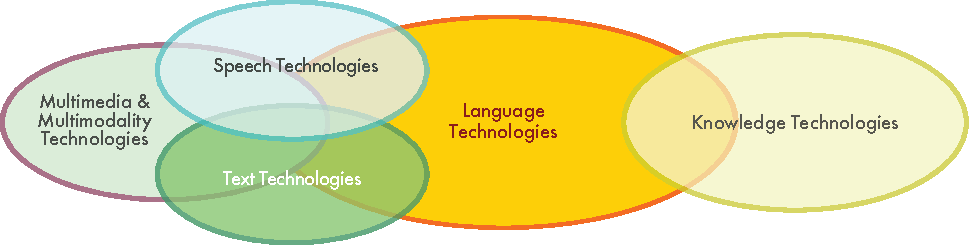
\includegraphics[width=\textwidth]{../_media/english/language_technologies}
  \caption{Language technology in context}
  \label{fig:ltincontext_en}
  \colorrule{grey3}{\textwidth}{1.5pt}
\end{figure*}

When we communicate, we combine language with other modes of communication and information media – for example speaking can involve gestures and facial expressions. Digital texts link to pictures and sounds. Movies may contain language in spoken and written form. In other words, speech and text technologies overlap and interact with other multimodal communication and multimedia technologies.\\ 
In this section, we will discuss the main application areas of language technology, i.\,e., language checking, web search, speech interaction, and machine translation. These applications and basic technologies include 

\begin{itemize}
\item spelling correction
\item authoring support
\item computer-assisted language learning
\item information retrieval 
\item information extraction
\item text summarisation
\item question answering
\item speech recognition 
\item speech synthesis 
\end{itemize}

Language technology is an established area of research with an extensive set of introductory literature. The interested reader is referred to the following references:  \cite{carstensen-etal1, jurafsky-martin01, manning-schuetze1, lt-world1, lt-survey1}.

Before discussing the above application areas, we will briefly describe the architecture of a typical LT system.

\subsection{Application Architectures}

Software applications for language processing typically consist of several components that mirror different aspects of language. While such applications are typically very complex, figure~\ref{fig:textprocessingarch_en} shows a highly simplified architecture of a typical text processing system. The first three modules handle the structure and meaning of the text input:

\begin{enumerate}
\item Pre-processing: cleans the data, analyses or removes formatting, detects the input languages, and so on.
\item Grammatical analysis: finds the verb, its objects, modifiers and other parts of speech; detects the sentence structure.
\item Semantic analysis: performs disambiguation (i.\,e., computes the appropriate meaning of words in a given context); resolves anaphora (i.\,e., which pronouns refer to which nouns in the sentence); represents the meaning of the sentence in a machine-readable way.
\end{enumerate}

After analysing the text, task-specific modules can perform other operations, such as automatic summarisation and database look-ups.

In the remainder of this section, we firstly introduce the core application areas for language technology, and follow this with a brief overview of the state of LT research and education today, and a description of past and present research programmes. Finally, we present an expert estimate of core LT tools and resources for Maltese in terms of various dimensions such as availability, maturity and quality. The general situation of LT for the Maltese language is summarised in a matrix (figure~\ref{fig:lrlttable_en}). Tools and resources that are underlined in the text can also be found in figure~\ref{fig:lrlttable_en} (p.~\pageref{fig:lrlttable_en}) at the end of this chapter. LT support for Maltese is also compared to other languages that are part of this series.

\begin{figure*}[htb]
  \colorrule{grey3}{\textwidth}{1.5pt}
  \center
  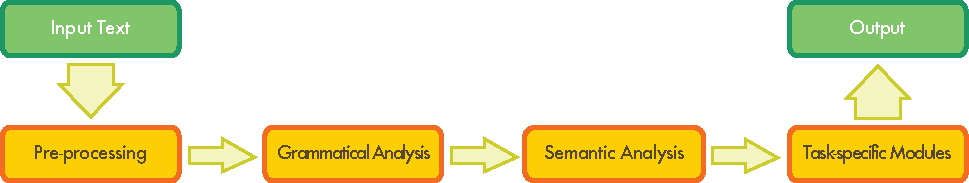
\includegraphics[width=\textwidth]{../_media/english/text_processing_app_architecture}
  \caption{A typical text processing architecture}
  \label{fig:textprocessingarch_en}
  \colorrule{grey3}{\textwidth}{1.5pt}
\end{figure*}

\subsection{Core Application Areas}

In this section, we focus on the most important LT tools and resources, and provide an overview of LT activities in Malta. 

\subsubsection{Language Checking}

Anyone who has used a word processor such as Microsoft Word knows that it has a spell checker that highlights spelling mistakes and proposes corrections. The first spelling correction programs compared a list of extracted words against a dictionary of correctly spelled words. Today these programs are far more sophisticated. Using language-dependent algorithms for \textbf{grammatical analysis}, they detect errors related to morphology (e.\,g., plural formation) as well as syntax–related errors, such as a missing verb or a conflict of verb-subject agreement (e.\,g., \textit{she *write a letter}). However, most spell checkers will not find any errors in the following text \cite{zar1}:

\begin{quote}
  I have a spelling checker,\\
  It came with my PC.\\
  It plane lee marks four my revue\\
  Miss steaks aye can knot sea.
\end{quote}

For handling this type of error, analysis of the context is needed in many cases, e.g., for deciding in which position in a Maltese verb the silent \emph{għ} has to be written, as in:

\begin{enumerate} %[(a)]
\item \emph{... in-negozjati li kien għamel il-Gvern ...}\\
`... the negotiations that the government had made...'

\item \emph{Pawlu, agħmel l-eżamijiet!} \\
`Paul, do the exams!'

\item *\emph{... in-negozjati li kien agħmel il-Gvern ...}
\end{enumerate}
 
Both \emph{għamel} `he made' and \emph{agħmel} `make!' are pronounced [ˈɐː.mɛl].

This either requires the formulation of language-specific grammar rules, involving a high degree of expertise and manual labour, or the use of a so-called statistical language model.  Such models calculate the probability of a particular word occurring in a specific environment (i.e., the preceding and following words). For example, \emph{kien għamel} is much more probable word sequence than \emph{kien agħmel}. A statistical language model can be automatically derived using a large amount of (correct) language data (i.e. a corpus). Up to now, these approaches have mostly been developed and evaluated using English language data. However, they do not necessarily transfer well to highly inflectional languages like Maltese, where a given word type, such as a verb, can yield a large number of orthographic forms. 

\begin{figure*}[htb]
  \colorrule{grey3}{\textwidth}{1.5pt}
  \center
  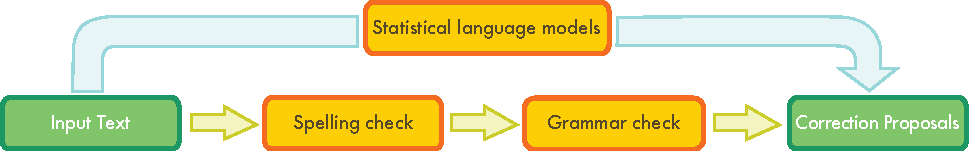
\includegraphics[width=\textwidth]{../_media/english/language_checking}
  \caption{Language checking (statistical; rule-based)}
  \label{fig:langcheckingaarch_en}
  \colorrule{grey3}{\textwidth}{1.5pt}
\end{figure*}

As with other languages, a means to determine whether a given string is a valid word is not a sufficient condition for spelling-error detection, but it is a necessary condition. As yet, no such means exists for Maltese, though various attempts have been made. 

One of the earliest was by \cite{Mangion:1999} using a rudimentary form of rule-driven morphological analysis. Essentially a word was considered valid if it could be derived by rule from a citation form found in a dictionary. The problem with this approach is that it requires a complete list of all citation forms, and of course, the rules have to be very accurate. Results were somewhat limited by the list of citation forms, which was incomplete, and the imperfect nature of the rules.

A second approach looked to statistics for a solution. The intuitive idea is that for a given language, certain sequences of characters are highly unlikely. In English, for example, we never find the sequence \emph{kk}, so if that occurs as a substring in a written word, we can guess, with a high degree of confidence, that the word is not valid. More generally, we can calculate the probability of any string as a function of the probabilities of all its substrings, adopting the principle that to count as a valid word, that probability must exceed a certain threshold.
A statistical spell checker making use of such a principle was developed by \cite{Mizzi:2001}. It did not require a lexicon, being based instead on the distribution of character n-grams found in a newspaper corpus. It became clear that for this approach to succeed (i) a more accurate language model was needed requiring more language data than was then available, and (ii) that string probability alone was insufficient to accurately classify an orthographic word as an error. As suggested above, other information is necessary, such as part of speech information from the surrounding context.

Other attempts to develop a spell-checker for Maltese include an online checker that has been developed by Ramon Casha of the Linux User Group\cite{Linux-spellcheck1}.  This is based on a wordlist of around 1 million word types originally collected from various corpora, and subsequently extended by various rules for handling inflections. Its accuracy has not been officially established. Microsoft has also been working on a spell checker for inclusion with their Maltese language interface pack though it is not clear when this will be released.

The use of language checking is not limited to word processing tools. Language checking is also applied to automatically correct queries sent to search engines, e.g. Google’s \emph{Did you mean…} suggestions. Other application areas include various kinds of authoring support software. 

As a result of the rapid increase in demand for technical products, many companies have begun to focus increasingly on the quality of technical documentation in the face of potential customer complaints about wrong linguistic usage and damage claims resulting from bad or badly understood instructions. Authoring support software can assist the writer of technical documentation to use vocabulary and sentence structures that are consistent with certain formally expressed rules and (corporate) terminology restrictions.

Authoring support software for Maltese does not at the moment exist but there would be considerable scope for the use of such software at the production end of Maltese. One of the reasons for the comparative scarcity of written Maltese content, in business correspondence for example, is that the production of correct Maltese text is difficult. Many competent native speakers are inclined to make mistakes when it comes to the written language and so they prefer to write in English. The availability of the right kind of simple authoring support tools could alleviate this problem.

An evolving area of language technology is \textbf{computer-assisted language learning} but apart from an interactive CD picture dictionary \cite{Sciriha:1997}, no such applications have been specifically developed for Maltese to date.


\subsubsection{Web Search}

\begin{figure*}[htb]
  \colorrule{grey3}{\textwidth}{1.5pt}
  \center
  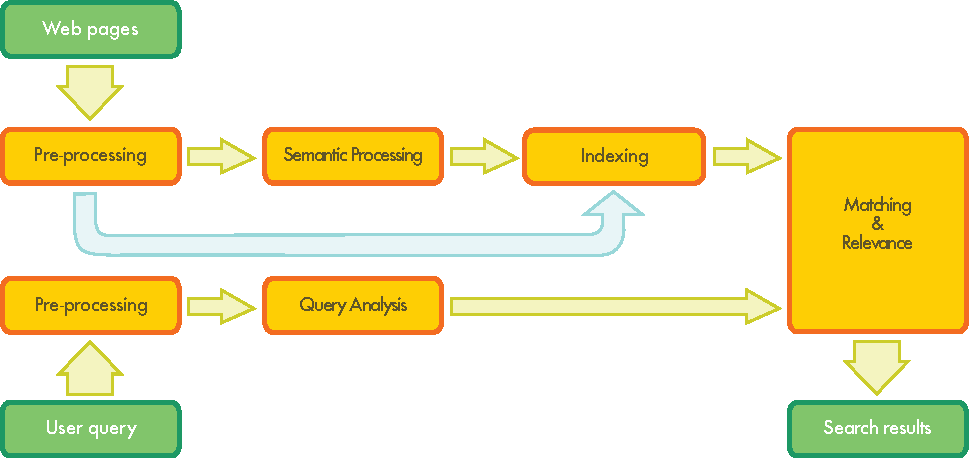
\includegraphics[width=\textwidth]{../_media/english/web_search_architecture}
  \caption{Web search}
  \label{fig:websearcharch_en}
  \colorrule{grey3}{\textwidth}{1.5pt}
 \end{figure*}

Search on the web, in intranets, or in digital libraries is probably the most widely used and yet underdeveloped language technology today. The search engine Google, which started in 1998, is nowadays used for about 80\% of all search queries world-wide\cite{spi1}. Since 2004, the verb \emph{to google} even has an entry in the \emph{Cambridge Advanced Learner’s Dictionary}. Neither the search interface nor the presentation of the retrieved results has significantly changed since the first version. In the current version, Google offers spelling correction for misspelled words and also, in 2009, incorporated basic semantic search capabilities into their algorithmic mix\cite{pc1}, which can improve search accuracy by analyzing the meaning of the query terms in context. The success story of Google shows that with a lot of data at hand and efficient indexing techniques a mainly statistical approach can lead to satisfactory results.  

However, for more sophisticated information requests, the integration of deeper linguistic knowledge is essential. In the research labs, experiments using machine-readable \underline{thesauri} and \underline{ontological language resources} like WordNet have shown improvements by allowing a page to be found on the basis of synonyms of the search terms, e.g. German \emph{Atomkraft, Kernenergie and Nuklearenergie} (atomic energy, atomic power, and nuclear energy) or even more loosely related terms. 

\boxtext{The next generation of search engines will have to include much more sophisticated language technology.}

The next generation of search engines will have to include much more sophisticated language technology. If a search query consists of a question or another type of sentence rather than a list of key-words, retrieving relevant answers to this query requires an analysis of this sentence at a syntactic and semantic level as well as the availability of an index that allows for a fast retrieval of the relevant documents. For example, imagine a user inputs the query ``Give me a list of all companies that were taken over by other companies in the last five years''. For a satisfactory answer, syntactic \underline{parsing} needs to be applied to analyze the grammatical structure of the sentence and determine that the user is looking for companies that have been taken over and not companies that took over others. Also, the expression \emph{last five years} needs to be processed in order to find out which years it refers to. 

Finally, the processed query needs to be matched against a huge amount of unstructured data in order to find the piece or pieces of information the user is looking for. This is commonly referred to as \underline{information retrieval} and involves the search for and ranking of relevant documents. In addition, generating a list of companies, we also need to extract the information that a particular string of words in a document actually refers to a company name. This kind of information is made available by so-called \underline{named-entity recognizers}. 

Even more demanding is the attempt to match a query to documents written in a different language. For \underline{cross-lingual information retrieval}, we have to automatically translate the query to all possible source languages and transfer the retrieved information back to the target language. The increasing percentage of data available in non-textual formats drives the demand for services enabling \underline{multimedia information retrieval}, i.e., information search on images, audio, and video data. For audio and video files, this involves a \underline{speech recognition} module to convert speech content into text or a phonetic representation, to which user queries can be matched.

In Malta, there are a number of search websites that are specifically oriented towards Malta\cite{philb1}. In addition there are a small number of Malta based SMEs that incorporate relatively sophisticated language processing techniques within search applications. Charonite\cite{charonite1}, for example, is a local SME dealing with search engine optimization. However, at the time of writing there are no commercially available search engines that are specifically oriented towards the Maltese language, apart from a prototype for cross lingual in-formation retrieval developed within the scope of LT4EL\cite{let1}, a European FP6 research project which used multilingual language technology tools and semantic encoding techniques for improving the retrieval of learning material. 

\subsubsection{Speech Interaction}

Speech interaction is one of many application areas that depend on speech technology, i.\,e., technologies for processing spoken language. Speech interaction technology is used to create interfaces that enable users to interact in spoken language instead of using a graphical display, keyboard and mouse.  Today, these voice user interfaces (VUI) are used for partially or fully automated telephone services provided by companies to customers, employees or partners. Business domains that rely heavily on VUIs include banking, supply chain, public transportation, and telecommunications. Other uses of speech interaction technology include interfaces to car navigation systems and the use of spoken language as an alternative to the graphical or touchscreen interfaces in smartphones.

\begin{figure*}[htb]
  \colorrule{grey3}{\textwidth}{1.5pt}
  \center
  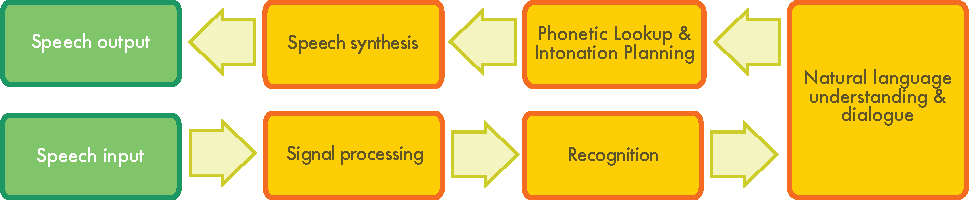
\includegraphics[width=\textwidth]{../_media/english/simple_speech-based_dialogue_architecture}
  \caption{Speech-based dialogue system}
  \label{fig:dialoguearch_en}
  \colorrule{grey3}{\textwidth}{1.5pt}
\end{figure*}

Speech interaction technology comprises four technologies: 

\begin{enumerate}
\item Automatic \textbf{speech recognition} (ASR) determines which words are actually spoken in a given sequence of sounds uttered by a user.  
\item Natural language understanding analyses the syntactic structure of a user’s utterance and interprets it according to the system in question.
\item Dialogue management determines which action to take given the user input and system functionality.   
\item \textbf{Speech synthesis} (text-to-speech or TTS) transforms the system’s reply into sounds for the user.
\end{enumerate}

One of the major challenges is to have an ASR system recognize the words uttered by a user as precisely as possible. This requires either a restriction of the range of possible user utterances to a limited set of keywords, or the manual creation of \underline{language models} that cover a large range of natural language user utterances. Whereas the former results in a rather rigid and inflexible usage of a VUI and possibly causes a poor user acceptance, the creation, tuning and maintenance of language models may increase the costs significantly. However, VUIs that employ language models and initially allow users to flexibly express their intentions – evoked, e.g., by a \emph{How may I help you} greeting – show both a higher automation rate and a higher user acceptance and may therefore be considered as advantageous over a less flexible directed dialogue approach. For the output part of a VUI, companies tend to use pre-recorded utterances of professional – ideally corporate – speakers. For static utterances, in which the wording does not depend on the particular contexts of use or the personal data of the given user, this will result in a rich user experience. However, the more dynamic content an utterance needs to consider, the more the user experience may suffer from a poor prosody resulting from concatenating single audio files. In contrast, today’s TTS systems prove superior, though optimizable, regarding the prosodic naturalness of dynamic utterances.  

\boxtext{Speech interaction is the basis for creating interfaces that allow a user to interact with spoken language instead of a graphical dis-play, keyboard and mouse.}

During last decade, the market for Speech interaction technology underwent a strong standardization with respect to the interfaces between different technology components, as well as to the standards for creating particular software artifacts for a given application. There also has been strong market consolidation within the last ten years, particularly in the field of ASR and TTS. Here, the national markets in the G20 countries – i.e. economically strong countries with a considerable population - are dominated by less than 5 players worldwide, with Nuance and Loquendo being the most prominent ones in Europe.

Most speech interaction technology development in Malta has concentrated on text-to-speech (TTS). Some pioneering work was initially carried out by \cite{Micallef:1997} and this was followed by a number of Master’s dissertations \cite{Farrugia:2005}. Some work on a web-based TTS system was initiated by \cite{Buhagiar-Micallef:2008}.

A significant recent development for Maltese speech synthesis was the winning of a government tender for the development of a speech synthesizer by the local company Crimson Wing Malta Ltd. This work is partly financed by the EU Regional Development fund and commissioned by the Maltese Foundation for Information Access (FITA). The prototype will be SAPI compliant and will include three voices (male, female, and child). According to a recent presentation \cite{Borg-et-al:2011} the work is advancing well and a prototype, expected in 2012, will be freely available for download. 

Work on speech recognition is less advanced. A prototype for recognizing numerals was created by \cite{Calleja:2002} in simple domains. With respect to speech, the fundamental problem remains a lack of suitably annotated data since this requires significant manual effort. Some attempts at automatic annotation have been made by \cite{Psaila:2008}. The creation of a corpus and descriptive framework for the study of Maltese intonation was initiated by the Institute of Linguistics carried out by \cite{Vella-Farrugia:2006}. It is expected that the corpora being developed by Crimson Wing will be made available for research.

Looking beyond the state of today’s technology, there will be significant changes due to the spread of smartphones as a new platform for managing customer relationships – in addition to the telephone, internet, and email channels. This tendency will also affect the employment of technology for Speech Interaction. On the one hand, demand for telephony-based VUIs will decrease in the long run. On the other hand, the usage of spoken language as a user-friendly input modality for smartphones will gain significant importance. This tendency is supported by the observable improvement of speaker-independent speech recognition accuracy for speech dictation services that are already offered as centralized services to smartphone users. Given this ‘outsourcing’ of the recognition task to the infrastructure of applications, the application-specific employment of linguistic core technologies will supposedly gain importance compared to the present situation.

\subsubsection{Machine Translation}

\begin{figure*}[htb]
  \colorrule{grey3}{\textwidth}{1.5pt}
  \center
  
\includegraphics[width=\textwidth]{../_media/english/machine_translation}
  \caption{Machine translation (statistical; rule-based)}
  \label{fig:mtarch_en}
  \colorrule{grey3}{\textwidth}{1.5pt}
\end{figure*}

The idea of using digital computers for translation of natural languages came up in 1946 by A. D. Booth and was followed by substantial funding for research in this area in the 1950s and beginning again in the 1980s. Nevertheless, \underline{Machine Translation} (MT) still fails to fulfill the high expectations it gave rise to in its early years.  

\boxtext{At its basic level, Machine Translation simply substitutes words in one natural language with words in another language.}

At its basic level, MT simply substitutes words in one natural language by words in another. This can be useful in subject domains with a very restricted, formulaic language, e.g., weather reports. However, for a good translation of less standardized texts, larger text units (phrases, sentences, or even whole passages) need to be matched to their closest counterparts in the target language. The major difficulty here lies in the fact that human language is ambiguous, which yields challenges on multiple levels, e.g., \underline{word sense disambiguation} on the lexical level (`Jaguar' can mean a car or an animal) or the attachment of prepositional phrases on the syntactic level as in:

\begin{enumerate} %[(a)]
\item \emph{Il-Kuntistabbli osserva lir-ragel bit-teleskopju.}\\
`The policeman observed the man with the telescope.'
\item \emph{Il-Kuntistabbli osserva lir-ragel bir-rivolver.}\\
`The policeman observed the man with the revolver.'
\end{enumerate}

One way of approaching the task is based on linguistic rules. For translations between closely related languages, a direct translation may be feasible in cases like the example above. But often rule-based (or knowledge-driven) systems analyze the input text and create an intermediary, symbolic representation, from which the text in the target language is generated. The success of these methods is highly dependent on the availability of extensive \underline{lexicons} with morphological, syntactic, and semantic information, and large sets of \underline{grammar rules} carefully designed by a skilled linguist.

Beginning in the late 1980s, as computational power increased and became less expensive, more interest was shown in statistical models for MT. The parameters of these statistical models are derived from the analysis of bilingual text \underline{corpora}, such as the Europarl parallel corpus, which contains the proceedings of the European Parliament in 11 European languages. Given enough data, statistical MT works well enough to derive an approximate meaning of a foreign language text. However, unlike knowledge-driven systems, statistical (or data-driven) MT often generates ungrammatical output. On the other hand, besides the advantage that less human effort is required for grammar writing, data-driven MT can also cover particularities of the language that go missing in knowledge-driven systems, for example idiomatic expressions. 

As the strengths and weaknesses of knowledge- and data-driven MT are complementary, researchers nowadays unanimously target hybrid approaches combining methodologies of both. This can be done in several ways. One is to use both knowledge- and data-driven systems and have a selection module decide on the best output for each sentence. However, for longer sentences, no result will be perfect. A better solution is to combine the best parts of each sentence from multiple outputs, which can be fairly complex, as corresponding parts of multiple alternatives are not always obvious and need to be aligned. 

\boxtext{The quality of MT systems is still considered to have huge improvement potential.}

In Malta work carried out in Machine Translation has been restricted to just a few Bachelors and Masters dissertations. A transfer system based on LFG was developed for English/Maltese by \cite{Farrugia:2000} and successfully translated weather forecasts. Later J. Bajada \cite{Bajada:2004, Bajada:2009} worked on statistical MT (SMT) with the emphasis on techniques for producing language and translation models. The earlier work concerned word-based models, whilst the latter developed techniques for gathering bilingual phrase data from a limited corpus.

Like in so many other areas, the underlying problem is a lack of sufficient quantities of suitably annotated bilingual data. For this reason, perhaps, the benchmark system against which to judge advances remains Google Translate.

The quality of MT systems is still considered to have huge improvement potential. Challenges include the adaptability of the language resources to a given subject domain or user area and the integration into existing workflows with term bases and translation memories. In addition, most of the current systems are English-centred and support only few languages from and into other languages, which leads to frictions in the total translation workflow, and e.g. forces MT users to learn different lexicon coding tools for different systems.

Evaluation campaigns allow for comparing the quality of MT systems, the various approaches and the status of MT systems for the different languages. Figure~\ref{fig:euromatrix_mt} (p.~\pageref{fig:euromatrix_mt}), which was prepared during the EC Euromatrix+ project, shows the pairwise performances obtained for 22 of the 23 official EU languages (Irish was not compared). The results are ranked according to a BLEU score, which indicates higher scores for better translations \cite{bleu1}. A human translator would normally achieve a score of around 80 points.

The best results (shown in green and blue) were achieved by languages that benefit from considerable research efforts, within coordinated programs, and from the existence of many parallel corpora (e.g. English, French, Dutch, Spanish, German), the worst (in red) by languages that did not benefit from similar efforts, or that are very different from other languages (e.g. Hungarian, Maltese, Finnish).

\subsection{Other Application Areas}

Building language technology applications involves a range of subtasks that do not always surface at the level of interaction with the user, but they provide significant service functionalities “behind the scenes” of the system in question. They all form important research issues that have now evolved into individual sub-disciplines of computational linguistics.  \underline{Question answering}, for example, is an active area of research for which annotated corpora have been built and scientific competitions have been initiated. The concept of question answering goes beyond keyword-based searches (in which the search engine responds by delivering a collection of potentially relevant documents) and enables users to ask a concrete question to which the system provides a single answer. For example:

\textit{Question: How old was Neil Armstrong when he stepped on the moon?}\\
\textit{Answer: 38.}

While question answering is obviously related to the core area of web search, it is nowadays an umbrella term for such research issues as which different types of questions exist, and how they should be handled; how a set of documents that potentially contain the answer can be analysed and compared (do they provide conflicting answers?); and how specific information (the answer) can be reliably extracted from a document without ignoring the context. 

\boxtext{Language technology applications often provide significant service functionalities "behind the scenes” of larger software systems.}

This is in turn related to the \underline{information extraction} (IE) task, an area that was extremely popular and influential at the time of the ``statistical turn'' in Computational Linguistics, in the early 1990s. IE aims at identifying specific pieces of information in specific classes of documents; this could be e.g. the detection of the key players in company takeovers as reported in newspaper stories. Another scenario that has been worked on is reports on terrorist incidents, where the problem is to map the text to a template specifying the perpetrator, the target, time and location of the incident, and the results of the incident. Domain-specific template-filling is the central characteristic of IE, which for this reason is another example of a ``behind the scenes'' technology that constitutes a well-demarcated research area but for practical purposes then needs to be embedded into a suitable application environment. 

Two ``borderline'' areas, which sometimes play the role of standalone application and sometimes that of supportive, ``under the hood'' component are \underline{text summarization} and \underline{text generation}. Summarization, obviously, refers to the task of making a long text short, and is offered for instance as a functionality within MS Word. It works largely on a statistical basis, by first identifying `important' words in a text (that is, for example, words that are highly frequent in this text but markedly less frequent in general language use) and then determining those sentences that contain many important words. These sentences are then marked in the document, or extracted from it, and are taken to constitute the summary. In this scenario, which is by far the most popular one, summarization equals sentence extraction: the text is reduced to a subset of its sentences. All commercial summarizers make use of this idea. An alternative approach, to which some research is devoted, is to actually synthesize \emph{new} sentences, i.e., to build a summary of sentences that need not show up in that form in the source text. This requires a certain amount of deeper understanding of the text and therefore is much less robust. All in all, a text generator is in most cases not a stand-alone application but embedded into a larger software environment, such as into the clinical information system where patient data is collected, stored and processed, and report generation is just one of many functionalities.

\subsection{Educational Programmes}

Language technology is a highly interdisciplinary field, involving the expertise of linguists, computer scientists, mathematicians, philosophers, psycholinguists, and neuroscientists, among others. 

In Malta the vast majority of research and education in LT has taken place at the University of Malta. However, it was established rather late. One reason for this was the late appearance of Computer Science as a curriculum subject at the University. The turbulent political leadership of the country during the 1970s and 1980s had not foreseen the information revolution to come and it was not until the early 1990s that an undergraduate option in Computing with Mathematics was offered through the Faculty of Science. 

The roots of change came in 1994, when a national strategic initiative was undertaken to recognize and strengthen the role of IT in commercial, political, and above all, educational sectors. One immediate consequence of this was the introduction of a substantial four-year Bachelors programme - the BSc. IT (Hons) - at University as well as the founding of a new Department of Computer Science and Artificial Intelligence (CSAI, renamed ``Department of Intelligent Computer Systems (ICS)'' in 2009). A course in NLP was included as an advanced option, and this led, four years later, to a series of undergraduate final year projects tackling language processing issues including computational approaches to Maltese \cite{Galea:1999, Mangion:1999, Farrugia:1999, Farrugia:2000, Mizzi:2000, Bajada:2004, Attard:2005, Farrugia:2008, Farrugia:2009, Vella:2010}. The Department of Computer Communications Engineering also participated in the programme, and this led to another set of undergraduate projects in speech technology.

Another important influence on research is the University’s Institute of Linguistics (IOL), founded in 1988 with the aim of teaching as well as promoting and coordinating research in both General and Applied Linguistics, furthering research involving the description of particular languages, not least Maltese, fostering the study of the various sub-fields of linguistics, and promoting interdisciplinary research involving academics in practical cooperation that cuts across departmental and faculty boundaries abroad. The Institute of Linguistics runs two undergraduate programmes: a B.A. in General Linguistics and a new B.Sc. in Human Language Technology which will be on offer in October 2011. It is also possible to do a Masters Degree and a Ph.D. in Linguistics with the Institute.

In 1997, an interdisciplinary group of computer scientists and linguists  embarked on Maltilex (M. Rosner, R. Fabri, J. Caruana, M. Montebello and others), a project to create a computational lexicon, which was sustained by a small grant from the University supported by the Mid-Med Bank. A simple web-based interface was developed to enable the creation and maintenance of entries, as reported in \cite{Rosner-et-al:1998} at the first ACL Workshop on Computational Approaches to Semitic Languages \cite{Rosner:1998}. Several thousand such entries were created by hand, but the project ran into legal problems, the compilation of entries having been largely inspired by Joseph Aquilina's existing paper dictionary \cite{Aquilina:1987}.

Effort then shifted from paper dictionaries to extraction of lexical entries from other sources. Two \cite{Dalli:2001, Attard:2006} used techniques based on alignment derived from bioinformatics to cluster lexical entries and this was used as a means of structuring the lexicon automatically. 

Despite lack of funding, the Maltilex effort continued in a some-what piecemeal fashion, supported by staff at the IOL and CSAI Department. It was not until 2005 that Malta's Council for Science and Technology (MCST) launched the country's first Research and Technology Development Initiative and a joint proposal for a Maltese Language Resource Server (MLRS) was accepted, providing sufficient financial support to employ a researcher full time be-tween 2006 and 2008. The project had the twin goals of creating both a lexicon and a corpus \cite{Rosner:2008}, and it laid the foundations for the present MLRS server.

The research mentioned above mainly deals with the written language. Two branches of speech-related work are also ongoing. 

The first, initiated from the signal-processing tradition within the Engineering Faculty, yielded a prototype speech synthesizer \cite{Micallef:1997}. His work has influenced several other projects aimed at improving speech synthesis from a low-resource perspective including \cite{Calleja:2002, Farrugia:2005, Camilleri:2010 , Borg-et-al:2011}.

The second tackles the issue of intonation \cite{Vella:2007} from a linguistic perspective. Some pioneering work to create a corpus and descriptive framework for the study of Maltese intonation was carried out by \cite{Vella-Farrugia:2006}. 

Outside Malta, two research groups that are in active collaboration with local LT-oriented efforts deserve a special mention.

At the University of Arizona, a group led by linguist Adam Ussishkin is particularly interested in the psycholinguistic issues pertaining to Semitic languages including Maltese. To study these issues an online corpus has been made available \cite{Ussishkin-et-al:2009}. 

At the University of Bremen, Prof. Thomas Stolz has been actively involved with the academic study of Maltese but is particularly known for having hosted the first conference on Maltese Linguistics in Bremen \cite{Comrie-et-al:2009}, founded a periodical\cite{GHILM2} and the International Association of Maltese Linguistics, also based in Bremen, that exists alongside the Malta-based Council for the Maltese Language.

As mentioned, the LT-sensitive communities existing at the University of Malta mainly inhabit the Faculty of ICT, the Institute of Linguistics. There is also a potential interest in Faculty of Arts (Department of Maltese) and other Humanities subjects though up until now computational linguistics tends to be regarded as an exotic topic located in the more scientific computer science faculties or in the humanities and, therefore, the research topics dealt with only overlap only partially.

Curiously, Malta does not lack for LT-related international events. LREC 2010 was held in Valletta, drawing 1200 participants. The annual EAMT conference was also held in Malta in 1994, and there have also been a number of smaller workshops held during the last 10 years.

\subsection{National Projects and Initiatives}

Malta joined the EU in 2004 and this event immediately conferred to Maltese the status of being an official EU language. With this status came new obligations - in particular to translate large quantities of official documents, and in addition, a recognition, at European level, that as a national language, it should have ``first-class'' status from a technological as well as a social perspective, and be accorded all the rights and privileges enjoyed by ``larger'' European languages (i.e. having larger numbers of native speakers). 

The government’s National IT Strategy 2008-10 included a number of objectives related to Maltese Language including (i) the development of online government in Maltese, (ii) creation of Maltese language tools, in collaboration with the University, and (iii) support for Maltese online communities. At the time of writing in 2011, not all the objectives have been realized. However the longer term effects of this strategy are beginning to take shape. 

Currently the language technology scene in Malta is under the influence of four main initiatives:
\begin{enumerate}
\item First of all, a government-supported project partly funded by EU regional development funds is under way to bring speech technology within the reach of disabled persons. The project is currently focused on Maltese speech synthesis, and at this point the relevant language models are in the process of being developed. The consortium, which consists of an SME (Crimson Wing Ltd), a foundation(FITA, Foundation for IT Access), and the University, has pledged that these resources will be made available for research purposes. It remains to be seen whether components of the speech synthesizer will be made available to resource sharing networks inspired by CLARIN and META.

\item Second, as is evident from the current report, Malta participates in METANET4U and is thus in receipt of significant EU funding aimed at the enhancement and distribution of resources and tools that are specifically for Maltese. The University of Malta is a member of META-NET and intends to fulfill its obligations towards the aims of META, particularly regarding the identification of stakeholders, actually and potential. 

\item Third, the Maltese Language Resource Server (MLRS) has come to fruition and significant efforts are under way at University, through the Institute of Linguistics (A. Gatt, C. Borg, R. Fabri) and the Department of Intelligent Computer Systems (M. Rosner), to maintain and develop it. Currently MLRS is online at http://mlrs.research.um.edu.mt. The corpus comprises some 80M words, and the system includes some basic services that include KWIC search and display, pattern-directed search, various kinds of statistical analysis etc. Further tools are currently planned including a part-of-speech tagger and a spell-checker.

\item Finally, a new undergraduate programme in Human Language Technology is destined to be launched by the Institute of Linguistics in October 2011. This will cover a full range of topics and will inevitably have a positive long-term effect on the study of Maltese from a computational perspective.
\end{enumerate}

Besides these, a project to develop an electronic version of the Aquilina dictionary \cite{Aquilina:1987} is currently in preparation. This is a collaborative effort between the University of Malta who are supplying the linguistic expertise, the University of Arizona, who have already digitized the dictionary into machine readable form, and the publishers Midsea Books of Valletta. The dual aims of the project are to update the content, and to confer upon researchers the flexibility to swiftly access the text. An effort is in progress locally, to organize the right level of lexicographic expertise necessary to update the content.

We should also mention Malta’s relationship to CLARIN, a proposed EU research infrastructure addressing the provision of language resources for the Humanities and Social Sciences. During specification phase, the University was able to participate thanks to a small support grant from the local Council for Science and Technology. However, it has turned out to be more challenging to secure the longer term funding required for the construction phase of CLARIN. Identification of a suitable government entity to take responsibility for the programme has so far been without success. Consequently, Malta’s future participation in the construction phase currently hangs in the balance.
  
\subsection{Availability of Tools and Resources}

Figure~\ref{fig:lrlttable_en} provides a rating for language technology support for the Maltese language. This rating of existing tools and resources was generated by leading experts in the field who provided estimates based on a scale from 0 (very low) to 6 (very high) using seven criteria.

\begin{figure*}[htb]
\centering
%\begin{tabular}{>{\columncolor{orange1}}p{.33\linewidth}ccccccc} % ORIGINAL
\begin{tabular}{>{\columncolor{orange1}}p{.33\linewidth}@{\hspace*{6mm}}c@{\hspace*{6mm}}c@{\hspace*{6mm}}c@{\hspace*{6mm}}c@{\hspace*{6mm}}c@{\hspace*{6mm}}c@{\hspace*{6mm}}c}
\rowcolor{orange1}
 \cellcolor{white}&\begin{sideways}\makecell[l]{Quantity}\end{sideways}
&\begin{sideways}\makecell[l]{\makecell[l]{Availability} }\end{sideways} &\begin{sideways}\makecell[l]{Quality}\end{sideways}
&\begin{sideways}\makecell[l]{Coverage}\end{sideways} &\begin{sideways}\makecell[l]{Maturity}\end{sideways} &\begin{sideways}\makecell[l]{Sustainability}\end{sideways} &\begin{sideways}\makecell[l]{Adaptability}\end{sideways} \\ \addlinespace
\multicolumn{8}{>{\columncolor{orange2}}l}{Language Technology: Tools, Technologies and Applications} \\ \addlinespace
Speech Recognition	&0.8 & 0.8 & 0.8 & 0.8 & 0.8 & 0.8 & 0.8 \\ \addlinespace
Speech Synthesis &2.4 & 0.8 & 3.2 & 3.2 & 2.4 & 2.4 & 2.4\\ \addlinespace
Grammatical analysis & 0.8 & 0.8 & 0.8 & 0.8 & 0.8 & 0.8 & 0.8\\ \addlinespace
Semantic analysis &0& 0& 0& 0& 0& 0& 0\\ \addlinespace
Text generation & 0& 0& 0& 0& 0& 0&0\\ \addlinespace
Machine translation &1.6 &1.6 & 1.6 & 1.6 & 1.6 & 1.6 & 1.6\\ \addlinespace
\multicolumn{8}{>{\columncolor{orange2}}l}{Language Resources: Resources, Data and Knowledge Bases} \\ \addlinespace
Text corpora &3.2 &3.2 &2.4 &2.4 &2.4 &3.2 &3.2\\ \addlinespace
Speech corpora &2.4 &0.8 &2.4 &1.6 &2.4 &2.4 &2.4\\ \addlinespace
Parallel corpora &3.2& 3.2& 2.4& 1.6& 1.6& 1.6& 1.6\\ \addlinespace
Lexical resources &2.4&2.4 &1.6 &2.4 &2.4 &2.4 &2.4\\ \addlinespace
Grammars &0& 0& 0&0 &0 &0 &0\\
\end{tabular}
\caption{State of language technology support for Maltese}
\label{fig:lrlttable_en}
\end{figure*}

For Maltese, the most evident characteristics revealed by the table are that
\begin{itemize}
\item many entries are blank, and
\item the highest grade scored is 3.2.
\end{itemize}

The fact that most entries are blank reflects the immature state of LT-related research and development in Malta. Although there are signs that the situation is improving, investment in language technology remains at a low level, and as a result, despite modest local achievements, the effort is fragmentary, both in terms of coverage of different areas, and in terms of sustainability of research: there have been too many projects involving just one area, just one researcher, and just one or two years. The collective efforts don’t add up as they should.

So what has been achieved? We can see by looking at the non-blank entries, whose average score yields the following ordering:

\begin{itemize}
\item Tools:
\begin{enumerate}
\item Tokenisation, Speech Synthesis
\item Speech Recognition
\end{enumerate}

\item Resources:
\begin{enumerate}
\item Reference Corpora
\item Parallel Corpora
\item Lexicons, Terminology (this should be understood to include wordlists)
\item Language Models
\end{enumerate}
\end{itemize}

With respect to tools:
Low level text extraction and processing tools are available, including a tokenizer. A POS-tagger is under development, but its performance is not state-of-the-art, pending further training with better annotated data. 
Higher level tools (syntactic or semantic analysis, classification tools, information extraction etc.) are entirely lacking. A consequence is that, for example, there are no treebanks available for Maltese.

Prototype speech recognition tools have been developed at University but are not readily available at the time of writing. However, the government-funded speech engine mentioned earlier should yield a working speech synthesizer by 2013. Whilst this is a very positive development, it is highly focused on the synthesis side of speech. Hardly any work on speech recognition is planned at this stage.

With respect to resources, the situation is a little more structured, in so far as there already exists MLRS, an extensible computational infrastructure in the form of a server providing the basic functionality to enable access over the web to available corpora, some services, and a rudimentary system to facilitate the submission of contributions. MLRS currently provides some very basic services for the extraction, representation, search and analysis of text.

The existing MLRS corpus is currently around 100 million tokens in length. It is predominantly textual and monolingual. It is also somewhat non-representative: there is an abundance of legalistic material, but a shortage of academic text and works of fiction.

As things stand, these materials can only be searched and analyzed through the server and cannot be accessed directly. The reasons are legalistic. With access restricted in this way, the complications of IPR and copyright have been neatly sidestepped. The price is that these complications will eventually have to be confronted in the future, and in fact META is in the process of formulating a set of licence agreements to suit the distribution of resources, like MLRS.


\subsection{Cross-language comparison}

The current state of LT support varies considerably from one language community to another. In order to compare the situation between languages, this section will present an evaluation based on two sample application areas (machine translation and speech processing) and one underlying technology (text analysis), as well as basic resources needed for building LT applications. The languages were categorised using the following five-point scale: 

\begin{enumerate}
\item Excellent support
\item Good support
\item Moderate support
\item Fragmentary support
\item Weak or no support
\end{enumerate}

LT support was measured according to the following criteria:

\textbf{Speech Processing:} Quality of existing speech recognition technologies, quality of existing speech synthesis technologies, coverage of domains, number and size of existing speech corpora, amount and variety of available speech-based applications.

\textbf{Machine Translation:} Quality of existing MT technologies, number of language pairs covered, coverage of linguistic phenomena and domains, quality and size of existing parallel corpora, amount and variety of available MT applications.

\textbf{Text Analysis:} Quality and coverage of existing text analysis technologies (morphology, syntax, semantics), coverage of linguistic phenomena and domains, amount and variety of available applications, quality and size of existing (annotated) text corpora, quality and coverage of existing lexical resources (e.\,g., WordNet) and grammars.

\textbf{Resources:} Quality and size of existing text corpora, speech corpora and parallel corpora, quality and coverage of existing lexical resources and grammars.

\begin{figure*}[tb]
  \small
  \centering
  \begin{tabular}
  { % defines color for each column.
  >{\columncolor{corange5}}p{.13\linewidth}@{\hspace{.040\linewidth}}
  >{\columncolor{corange4}}p{.13\linewidth}@{\hspace{.040\linewidth}}
  >{\columncolor{corange3}}p{.13\linewidth}@{\hspace{.040\linewidth}}
  >{\columncolor{corange2}}p{.13\linewidth}@{\hspace{.040\linewidth}}
  >{\columncolor{corange1}}p{.13\linewidth} 
  }
  \multicolumn{1}{>{\columncolor{white}}c@{\hspace{.040\linewidth}}}{\textbf{Excellent}} & 
  \multicolumn{1}{@{}>{\columncolor{white}}c@{\hspace{.040\linewidth}}}{\textbf{Good}} &
  \multicolumn{1}{@{}>{\columncolor{white}}c@{\hspace{.040\linewidth}}}{\textbf{Moderate}} &
  \multicolumn{1}{@{}>{\columncolor{white}}c@{\hspace{.040\linewidth}}}{\textbf{Fragmentary}} &
  \multicolumn{1}{@{}>{\columncolor{white}}c}{\textbf{Weak/no}} \\ 
  \multicolumn{1}{>{\columncolor{white}}c@{\hspace{.040\linewidth}}}{\textbf{support}} & 
  \multicolumn{1}{@{}>{\columncolor{white}}c@{\hspace{.040\linewidth}}}{\textbf{support}} &
  \multicolumn{1}{@{}>{\columncolor{white}}c@{\hspace{.040\linewidth}}}{\textbf{support}} &
  \multicolumn{1}{@{}>{\columncolor{white}}c@{\hspace{.040\linewidth}}}{\textbf{support}} &
  \multicolumn{1}{@{}>{\columncolor{white}}c}{\textbf{support}} \\ \addlinespace
  
& \vspace*{0.5mm}English
& \vspace*{0.5mm}
Czech \newline 
Dutch \newline 
Finnish \newline 
French \newline 
German \newline   
Italian \newline  
Portuguese \newline 
Spanish \newline
& \vspace*{0.5mm}Basque \newline 
Bulgarian \newline 
Catalan \newline 
Danish \newline 
Estonian \newline 
Galician\newline 
Greek \newline  
Hungarian  \newline
Irish \newline  
Norwegian \newline 
Polish \newline 
Serbian \newline 
Slovak \newline 
Slovene \newline 
Swedish \newline
& \vspace*{0.5mm}
Croatian \newline 
Icelandic \newline  
Latvian \newline 
Lithuanian \newline 
Maltese \newline 
Romanian\\
\end{tabular}
\caption{Speech processing: state of language technology support for 30 European languages}
\label{fig:speech_cluster_en}
\end{figure*}

\begin{figure*}[tb]
  \small
  \centering
  \begin{tabular}
  { % defines color for each column.
  >{\columncolor{corange5}}p{.13\linewidth}@{\hspace{.040\linewidth}}
  >{\columncolor{corange4}}p{.13\linewidth}@{\hspace{.040\linewidth}}
  >{\columncolor{corange3}}p{.13\linewidth}@{\hspace{.040\linewidth}}
  >{\columncolor{corange2}}p{.13\linewidth}@{\hspace{.040\linewidth}}
  >{\columncolor{corange1}}p{.13\linewidth} 
  }
  \multicolumn{1}{>{\columncolor{white}}c@{\hspace{.040\linewidth}}}{\textbf{Excellent}} & 
  \multicolumn{1}{@{}>{\columncolor{white}}c@{\hspace{.040\linewidth}}}{\textbf{Good}} &
  \multicolumn{1}{@{}>{\columncolor{white}}c@{\hspace{.040\linewidth}}}{\textbf{Moderate}} &
  \multicolumn{1}{@{}>{\columncolor{white}}c@{\hspace{.040\linewidth}}}{\textbf{Fragmentary}} &
  \multicolumn{1}{@{}>{\columncolor{white}}c}{\textbf{Weak/no}} \\ 
  \multicolumn{1}{>{\columncolor{white}}c@{\hspace{.040\linewidth}}}{\textbf{support}} & 
  \multicolumn{1}{@{}>{\columncolor{white}}c@{\hspace{.040\linewidth}}}{\textbf{support}} &
  \multicolumn{1}{@{}>{\columncolor{white}}c@{\hspace{.040\linewidth}}}{\textbf{support}} &
  \multicolumn{1}{@{}>{\columncolor{white}}c@{\hspace{.040\linewidth}}}{\textbf{support}} &
  \multicolumn{1}{@{}>{\columncolor{white}}c}{\textbf{support}} \\ \addlinespace
  
& \vspace*{0.5mm} English 
& \vspace*{0.5mm} 
French \newline 
Spanish
& \vspace*{0.5mm}
Catalan \newline 
Dutch \newline 
German \newline 
Hungarian \newline
Italian \newline 
Polish \newline 
Romanian \newline 
& \vspace*{0.5mm}Basque \newline 
Bulgarian \newline 
Croatian \newline 
Czech \newline
Danish \newline 
Estonian \newline 
Finnish \newline 
Galician \newline 
Greek \newline 
Icelandic \newline 
Irish \newline 
Latvian \newline 
Lithuanian \newline 
Maltese \newline 
Norwegian \newline 
Portuguese \newline 
Serbian \newline 
Slovak \newline 
Slovene \newline 
Swedish \newline 
\end{tabular}
\caption{Machine translation: state of language technology support for 30 European languages}
\label{fig:mt_cluster_en}
\end{figure*}

\begin{figure*}[tb]
  \small
  \centering
  \begin{tabular}
  { % defines color for each column.
  >{\columncolor{corange5}}p{.13\linewidth}@{\hspace{.040\linewidth}}
  >{\columncolor{corange4}}p{.13\linewidth}@{\hspace{.040\linewidth}}
  >{\columncolor{corange3}}p{.13\linewidth}@{\hspace{.040\linewidth}}
  >{\columncolor{corange2}}p{.13\linewidth}@{\hspace{.040\linewidth}}
  >{\columncolor{corange1}}p{.13\linewidth} 
  }
  \multicolumn{1}{>{\columncolor{white}}c@{\hspace{.040\linewidth}}}{\textbf{Excellent}} & 
  \multicolumn{1}{@{}>{\columncolor{white}}c@{\hspace{.040\linewidth}}}{\textbf{Good}} &
  \multicolumn{1}{@{}>{\columncolor{white}}c@{\hspace{.040\linewidth}}}{\textbf{Moderate}} &
  \multicolumn{1}{@{}>{\columncolor{white}}c@{\hspace{.040\linewidth}}}{\textbf{Fragmentary}} &
  \multicolumn{1}{@{}>{\columncolor{white}}c}{\textbf{Weak/no}} \\ 
  \multicolumn{1}{>{\columncolor{white}}c@{\hspace{.040\linewidth}}}{\textbf{support}} & 
  \multicolumn{1}{@{}>{\columncolor{white}}c@{\hspace{.040\linewidth}}}{\textbf{support}} &
  \multicolumn{1}{@{}>{\columncolor{white}}c@{\hspace{.040\linewidth}}}{\textbf{support}} &
  \multicolumn{1}{@{}>{\columncolor{white}}c@{\hspace{.040\linewidth}}}{\textbf{support}} &
  \multicolumn{1}{@{}>{\columncolor{white}}c}{\textbf{support}} \\ \addlinespace

& \vspace*{0.5mm}English
& \vspace*{0.5mm}
  Dutch \newline 
  French \newline 
  German \newline 
  Italian \newline 
  Spanish
& \vspace*{0.5mm}Basque \newline 
  Bulgarian \newline 
  Catalan \newline 
  Czech \newline 
  Danish \newline 
  Finnish \newline 
  Galician \newline 
  Greek \newline 
  Hungarian \newline 
  Norwegian \newline 
  Polish \newline 
  Portuguese \newline 
  Romanian \newline 
  Slovak \newline 
  Slovene \newline 
  Swedish \newline 
& \vspace*{0.5mm}
  Croatian \newline 
  Estonian \newline 
  Icelandic \newline 
  Irish \newline 
  Latvian \newline 
  Lithuanian \newline 
  Maltese \newline 
  Serbian \\
  \end{tabular}
\caption{Text analysis: state of language technology support for 30 European languages}
\label{fig:text_cluster_en}
\end{figure*}

\begin{figure*}[tb]
  \small
  \centering
  \begin{tabular}
  { % defines color for each column.
  >{\columncolor{corange5}}p{.13\linewidth}@{\hspace{.040\linewidth}}
  >{\columncolor{corange4}}p{.13\linewidth}@{\hspace{.040\linewidth}}
  >{\columncolor{corange3}}p{.13\linewidth}@{\hspace{.040\linewidth}}
  >{\columncolor{corange2}}p{.13\linewidth}@{\hspace{.040\linewidth}}
  >{\columncolor{corange1}}p{.13\linewidth} 
  }
  \multicolumn{1}{>{\columncolor{white}}c@{\hspace{.040\linewidth}}}{\textbf{Excellent}} & 
  \multicolumn{1}{@{}>{\columncolor{white}}c@{\hspace{.040\linewidth}}}{\textbf{Good}} &
  \multicolumn{1}{@{}>{\columncolor{white}}c@{\hspace{.040\linewidth}}}{\textbf{Moderate}} &
  \multicolumn{1}{@{}>{\columncolor{white}}c@{\hspace{.040\linewidth}}}{\textbf{Fragmentary}} &
  \multicolumn{1}{@{}>{\columncolor{white}}c}{\textbf{Weak/no}} \\ 
  \multicolumn{1}{>{\columncolor{white}}c@{\hspace{.040\linewidth}}}{\textbf{support}} & 
  \multicolumn{1}{@{}>{\columncolor{white}}c@{\hspace{.040\linewidth}}}{\textbf{support}} &
  \multicolumn{1}{@{}>{\columncolor{white}}c@{\hspace{.040\linewidth}}}{\textbf{support}} &
  \multicolumn{1}{@{}>{\columncolor{white}}c@{\hspace{.040\linewidth}}}{\textbf{support}} &
  \multicolumn{1}{@{}>{\columncolor{white}}c}{\textbf{support}} \\ \addlinespace
    
& \vspace*{0.5mm}English
& \vspace*{0.5mm} 
    Czech \newline 
    Dutch \newline 
    French \newline 
    German \newline 
    Hungarian \newline
    Italian \newline
    Polish \newline
    Spanish \newline
    Swedish \newline 
& \vspace*{0.5mm} Basque\newline 
    Bulgarian\newline 
    Catalan \newline 
    Croatian \newline 
    Danish \newline 
    Estonian \newline 
    Finnish \newline 
    Galician \newline 
    Greek \newline 
    Norwegian \newline 
    Portuguese \newline 
    Romanian \newline 
    Serbian \newline 
    Slovak \newline 
    Slovene \newline
&  \vspace*{0.5mm}
    Icelandic \newline 
    Irish \newline 
    Latvian \newline 
    Lithuanian \newline 
    Maltese  \\
  \end{tabular}
  \caption{Speech and text resources: State of support for 30 European languages}  
  \label{fig:resources_cluster_en}
\end{figure*}


Tables~\ref{fig:speech_cluster_en} to~\ref{fig:resources_cluster_en} show that the Maltese language has only low to medium LT support and thus compares well with other less spoken languages of Europe. LT resources and tools for Maltese clearly do not yet reach the quality and coverage of comparable resources and tools for “major” languages like German, and certainly not that of those for the English language, which is in the lead in almost all LT areas. And there are still plenty of gaps in English language resources with regard to high quality applications. 


\subsection{Conclusions}

\emph{In this series of white papers, we have made an important initial effort to assess language technology support for 30 European languages, and provide a high-level comparison across these languages. By identifying the gaps, needs and deficits, the European language technology community and related stakeholders are now in a position to design a large scale research and development programme aimed at building a truly multilingual, technology-enabled Europe.}

The results of this white paper series show that there is a dramatic difference in language technology support for the various European languages. While there are good quality software and resources available for some languages and application areas, others, usually smaller languages, have substantial gaps. Many languages lack basic technologies for text analysis and the essential resources. Others have basic tools and resources but the implementation of for example semantic methods is still far away. Therefore a large-scale effort is needed to attain the ambitious goal of providing high-quality language technology support for all European languages, for example through high quality machine translation. 

In the case of the German language, we can be cautiously optimistic about the current state of language technology support. There is a viable LT research community in Germany, Austria and Switzerland, which has been supported in the past by large research programmes, many of them in cooperation with industrial players such as Philips and IBM. And a number of large-scale resources and state-of-the-art technologies have been produced for Standard German. However, the scope of the resources and the range of tools are still very limited when compared to English, and they are simply not sufficient in quality and quantity to develop the kind of technologies required to support a truly multilingual knowledge society.

Nor can we simply transfer technologies already developed and optimised for the English language to handle German. English-based systems for parsing (syntactic and grammatical analysis of sentence structure) typically perform far less well on German texts, due to the specific characteristics of the German language.

The German language technology industry is currently fragmented and disorganised. Most large companies have either stopped or severely cut their LT efforts, leaving the field to a number of specialised SMEs that are not robust enough to address the internal and the global market with a sustained strategy. 

Our findings lead to the conclusion that the only way forward is to make a substantial effort to create language technology resources for German, as a means to drive forward research, innovation and development. The need for large amounts of data and the extreme complexity of language technology systems makes it vital to develop an infrastructure and a coherent research organisation to spur greater sharing and cooperation.

Finally there is a lack of continuity in research and development funding. Short-term coordinated programmes tend to alternate with periods of sparse or zero funding. In addition, there is an overall lack of coordination with programmes in other EU countries and at the European Commission level.

The long term goal of META-NET is to enable the creation of high-quality language technology for all languages. This requires all stakeholders - in politics, research, business, and society - to unite their efforts. The resulting technology will help tear down existing barriers and build bridges between Europe’s languages, paving the way for political and economic unity through cultural diversity. 
\end{multicols}

\clearpage

\ssection[About META-NET]{About META-NET}

\begin{multicols}{2}
META-NET is a Network of Excellence funded by the European Commission. The network currently consists of 54 members from 33 European countries. META-NET fosters the Multilingual Europe Technology Alliance (META), a growing community of language technology professionals and organisations in Europe. META-NET cooperates with other initiatives like the Common Language Resources and Technology Infrastructure (CLARIN), which is helping establish digital humanities research in Europe. META-NET fosters the technological foundations for a truly multilingual European information society that:

\begin{itemize}
\item makes communication and cooperation possible across languages;
\item provides equal access to information and knowledge in any language;
\item offers advanced and affordable networked information technology to European citizens.
\end{itemize}

META-NET stimulates and promotes multilingual technologies for all European languages. The technologies enable automatic translation, content production, information processing and knowledge management for a wide variety of applications and subject domains. The network wants to improve current approaches, so better communication and cooperation across languages can take place. Europeans have an equal right to information and knowledge regardless of language.

META-NET launched on 1 February 2010 with the goal of advancing research in language technology (LT). The network supports a Europe that unites as a single digital market and information space. META-NET has conducted several activities that further its goals. META-VISION, META-SHARE and META-RESEARCH are the network’s three lines of action.

\textbf{META-VISION} fosters a dynamic and influential stakeholder community that unites around a shared vision and a common strategic research agenda (SRA). The main focus of this activity is to build a coherent and cohesive LT community in Europe by bringing together representatives from highly fragmented and diverse groups of stakeholders. In the first year of META-NET, presentations at the FLaReNet Forum (Spain), Language Technology Days (Luxembourg), JIAMCATT 2010 (Luxembourg), LREC 2010 (Malta), EAMT 2010 (France) and ICT 2010 (Belgium) centred on public outreach. According to initial estimates, META-NET has already contacted more than 2,500 LT professionals to develop its goals and visions with them. At the META-FORUM 2010 event in Brussels, META-NET communicated the initial results of its vision building process to more than 250 participants. In a series of interactive sessions, the participants provided feedback on the visions presented by the network. 

\textbf{META-SHARE} creates an open, distributed facility for exchanging and sharing resources. The peer-to-peer network of repositories will contain language data, tools and web services that are documented with high-quality metadata and organised in standardised categories. The resources can be readily accessed and uniformly searched. The available resources include free, open source materials as well as restricted, commercially available, fee-based items. META-SHARE targets existing language data, tools and systems as well as new and emerging products that are required for building and evaluating new technologies, products and services. The reuse, combination, repurposing and re-engineering of language data and tools plays a crucial role. META-SHARE will eventually become a critical part of the LT marketplace for developers, localisation experts, researchers, translators and language professionals from small, mid-sized and large enterprises. META-SHARE addresses the full development cycle of LT—from research to innovative products and services. A key aspect of this activity is establishing META-SHARE as an important and valuable part of a European and global infrastructure for the LT community. 

\textbf{META-RESEARCH} builds bridges to related technology fields. This activity seeks to leverage advances in other fields and to capitalise on innovative research that can benefit language technology. In particular, this activity wants to bring more semantics into machine translation (MT), optimise the division of labour in hybrid MT, exploit context when computing automatic translations and prepare an empirical base for MT. META-RESEARCH is working with other fields and disciplines, such as machine learning and the Semantic Web community. META-RESEARCH focuses on collecting data, preparing data sets and organising language resources for evaluation purposes; compiling inventories of tools and methods; and organising workshops and training events for members of the community. This activity has already clearly identified aspects of MT where semantics can impact current best practices. In addition, the activity has created recommendations on how to approach the problem of integrating semantic information in MT. META-RESEARCH is also finalising a new language resource for MT, the Annotated Hybrid Sample MT Corpus, which provides data for English-German, English-Spanish and English-Czech language pairs. META-RESEARCH has also developed software that collects multilingual corpora that are hidden on the Web.
\end{multicols}

\cleardoublepage

\appendix
\addtocontents{toc}{\protect\bigskip}

\bsection[Referenzi  -- References]{Referenzi --- References}
\bibliographystyle{plain}
\bibliography{references}
  
\cleardoublepage

\bsection[Membri ta' META-NET -- META-NET Members]{Membri ta' META-NET --- META-NET Members}
\label{metanetmembers}

\small
\begin{longtable}{llp{105mm}}
  Awstrija & \textcolor{grey1}{Austria} & Zentrum für Translationswissenschaft, Universität Wien: Gerhard Budin\\ \addlinespace
  Belġju & \textcolor{grey1}{Belgium} & Computational Linguistics and Psycholinguistics Research Centre, Univ. of Antwerp: Walter Daelemans\\ \addlinespace
  & & Centre for Proc. Speech and Images, Univ. of Leuven: Dirk van Compernolle \\ \addlinespace
  Bulgarija & \textcolor{grey1}{Bulgaria} & Inst. for Bulgarian Lang., Bulgarian Academy of Sciences: Svetla Koeva \\ \addlinespace
  Ċekja & \textcolor{grey1}{Czech Republic} & Inst. of Formal and Applied Linguistics, Charles Univ. in Prague: Jan Hajic \\ \addlinespace
  Ċipru & \textcolor{grey1}{Cyprus} & Lang. Centre, School of Humanities: Jack Burston \\ \addlinespace
  Danimarka &  \textcolor{grey1}{Denmark} & Centre for Lang. Technology, Univ. of Copenhagen: Bolette Sandford Pedersen, Bente Maegaard\\ \addlinespace
  Estonja & \textcolor{grey1}{Estonia} & Inst. of Computer Science, Univ. of Tartu: Tiit Roosmaa\\ \addlinespace
  Finlandja & \textcolor{grey1}{Finland} & Computational Cognitive Systems Research Group, Aalto Univ.: Timo Honkela\\ \addlinespace
  & & Dept. of General Linguistics, Univ. of Helsinki: Kimmo Koskenniemi, Krister Linden \\ \addlinespace
  Franza & \textcolor{grey1}{France} & Centre National de la Recherche Scientifique, Laboratoire d'Informatique pour la Mécanique et les Sciences de l'Ingénieur: Joseph Mariani \\ \addlinespace
  & & Evaluations and Lang. Resources Distribution Agency: Khalid Choukri\\ \addlinespace 
  Ġermanja & \textcolor{grey1}{Germany} & DFKI (German Research Centre for Artificial Intelligence): Hans Uszkoreit, Georg Rehm\\ \addlinespace
  & & Human Lang. Technology and Pattern Recognition, RWTH Aachen Univ.: Hermann Ney \\ \addlinespace
  & & Dept. of Computational Linguistics, Saarland Univ.: Manfred Pinkal\\ \addlinespace 
  Gran Brittanja & \textcolor{grey1}{UK} & Inst. for Lang., Cognition and Computation, Center for Speech Technology Research, Univ. of Edinburgh: Steve Renals \\ \addlinespace 
  & & Research Inst. of Informatics and Lang. Proc., Univ. of Wolverhampton: Ruslan Mitkov \\ \addlinespace 
  & & School of Computer Science, Univ. of Manchester: Sophia Ananiandou \\ \addlinespace 
  Greċja & \textcolor{grey1}{Greece} & Inst. for Lang. and Speech Proc., R.C. “Athena”: Stelios Piperidis\\ \addlinespace
  Irlanda & \textcolor{grey1}{Ireland} & School of Computing, Dublin City Univ.: Josef van Genabith\\ \addlinespace
  Islanda & \textcolor{grey1}{Iceland} & School of Humanities, Univ. of Iceland: Eirikur Rögnvaldsson\\ \addlinespace
  Isvezja & \textcolor{grey1}{Sweden} & Dept. of Swedish Lang., Univ. of Gothenburg: Lars Borin \\ \addlinespace 
  Isvizzera & \textcolor{grey1}{Switzerland} & Idiap Research Inst.: Hervé Bourlard \\ \addlinespace 
  Italja & \textcolor{grey1}{Italy} & Consiglio Nazionale Ricerche, Istituto di Linguistica Computazionale “Antonio Zampolli”: Nicoletta Calzolari\\ \addlinespace
  & & Human Lang. Technology, Fondazione Bruno Kessler: Bernardo Magnini\\ \addlinespace 
  Kroazja & \textcolor{grey1}{Croatia} & Inst. of Linguistics, Faculty of Humanities and Social Science, Univ. of Zagreb: Marko Tadić \\ \addlinespace
  Latvja & \textcolor{grey1}{Latvia} & Tilde: Andrejs Vasiljevs\\ \addlinespace 
  & & Inst. of Mathematics and Computer Science, Univ. of Latvia: Inguna Skadina\\ \addlinespace
  Litwanja & \textcolor{grey1}{Lithuania} & Inst. of the Lithuanian Lang.: Jolanta Zabarskaitė\\ \addlinespace
  Lussemburgu & \textcolor{grey1}{Luxembourg} & Arax Ltd.: Vartkes Goetcherian\\ \addlinespace
  Malta & \textcolor{grey1}{Malta} & Dept. Intelligent Computer Systems, Univ. of Malta: Mike Rosner\\ \addlinespace
  Norveġja & \textcolor{grey1}{Norway} & Dept. of Linguistic, Univ. of Bergen: Koenraad De Smedt\\ \addlinespace 
  & & Dept. of Informatics, Lang. Technology Group, Univ. of Oslo: Stephan Oepen \\ \addlinespace 
  Olanda & \textcolor{grey1}{Netherlands} & Utrecht Inst. of Linguistics, Utrecht Univ.: Jan Odijk\\ \addlinespace 
  & & Computational Linguistics, Univ. of Groningen: Gertjan van Noord\\ \addlinespace
  Polonja & \textcolor{grey1}{Poland} & Inst. of Computer Science, Polish Academy of Sciences: Adam Przepiórkowski, Maciej Ogrodniczuk \\ \addlinespace
  & & Univ. of Łódź: Barbara Lewandowska-Tomaszczyk, Piotr Pęzik\\ \addlinespace
  & & Dept. of Computer Linguistics and Artificial Intelligence, Adam Mickiewicz Univ.: Zygmunt Vetulani \\ \addlinespace
  Portugall & \textcolor{grey1}{Portugal} & Dept. of Informatics, Univ. of Lisbon: Antonio Branco\\ \addlinespace
  & & Spoken Lang. Systems Lab., Inst. for Systems Engineering and Computers: Isabel Trancoso \\ \addlinespace
  Rumanija & \textcolor{grey1}{Romania} & Research Inst. for Artificial Intelligence, Romanian Academy of Sciences: Dan Tufis \\ \addlinespace
  & & Faculty of Computer Science, Univ. Alexandru Ioan Cuza: Dan Cristea \\ \addlinespace
  Serbja & \textcolor{grey1}{Serbia} & Faculty of Mathematics, Belgrade Univ.: Dusko Vitas, Cvetana Krstev, Ivan Obradovic \\ \addlinespace
  & & Pupin Inst.: Sanja Vranes \\ \addlinespace  
  Slovakkja & \textcolor{grey1}{Slovakia} & Ludovit Stur Inst. of Linguistics, Slovak Academy of Sciences: Radovan Garabik \\ \addlinespace 
  Slovenja & \textcolor{grey1}{Slovenia} & Jozef Stefan Inst.: Marko Grobelnik \\ \addlinespace 
  Spanja & \textcolor{grey1}{Spain} & Barcelona Media: Toni Badia \\ \addlinespace 
  & & Institut Universitari de Lingüistica Aplicada, Univ. Pompeu Fabra: Núria Bel \\ \addlinespace 
  & & Aholab Signal Proc. Lab., Univ. of the Basque Country: Inma Hernaez Rioja \\ \addlinespace 
  & & Center for Lang. and Speech Technologies and Applications, Technical Univ. of Catalonia: Asunción Moreno \\ \addlinespace 
  & & Dept. of Signal Proc. and Communications, Univ. of Vigo: Carmen García Mateo \\ \addlinespace 
  Ungerija & \textcolor{grey1}{Hungary} & Research Inst. for Linguistics, Hungarian Academy of Sciences: Tamás Váradi\\  \addlinespace
  & & Dept. of Telecommunications and Media Informatics, Budapest Univ. of Technology and Economics: Géza Németh and Gábor Olaszy\\ \addlinespace
\end{longtable}
\normalsize

\renewcommand*{\figureformat}{}
\renewcommand*{\captionformat}{}

\begin{figure*}[htbp]
  \center
  %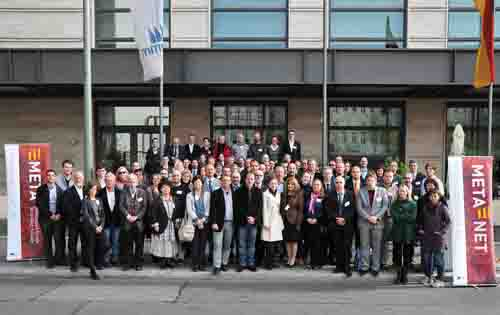
\includegraphics[width=\textwidth]{../_media/meta-net_team.jpg}
   \fbox{Dummy -- we'll include the group photo of our META-NET meeting in Berlin here}
  \caption{Kważi 100 esperti tat-teknoloġija lingwistika -- rappreżentanti tal-pajjiżi u tal-lingwi li huma rappreżentati f'META-NET -- ddiskutew u ffinalizzaw ir-riżultati ewlenin u l-messaġġi ta' Serje ta’ White Papers tal-META-NET f'laqgħa f'Berlin, fil-Ġermanja, dwar Ottubru 21/22, 2011. --- \textcolor{grey1}{About 100 language technology experts -- representatives of the countries and languages represented in META-NET -- discussed and finalised the key results and messages of the White Paper Series at a META-NET meeting in Berlin, Germany, on October 21/22, 2011.}}
\end{figure*}

\cleardoublepage

\bsection[Is-Serje ta’ White Papers ta' META-NET -- The META-NET White Paper Series]{Is-Serje ta’ White Papers ta' META-NET --- The META-NET\ \ \ \ \ \ White Paper Series}
\label{whitepaperseries}

\vspace*{-5mm}
\centering
  \setlength{\tabcolsep}{2em}
  \begin{tabularx}{\textwidth}{lllll} \toprule\addlinespace
  %\begin{tabulary}{170mm}{LLL} \toprule
  & Bask & Basque & euskara\\
& Bulgaru & Bulgarian & български\\
& Ċek & Czech & čeština\\
& Daniż & Danish & dansk\\
& Estonjan & Estonian & eesti\\
& Finlandiż & Finnish & suomi\\
& Franċiż & French & français\\
& Ġermaniż & German & Deutsch\\
& Galizjan & Galician & galego\\
& Grieg & Greek & ελληνικά\\
& Ingliż & English & English\\
& Irlandiż & Irish & Gaeilge\\
& Islandiż & Icelandic & íslenska\\
& Katalan & Catalan & català\\
& Kroat & Croatian & hrvatski\\
& Latvjan & Latvian & latviešu valoda\\
& Litwan & Lithuanian & lietuvių kalba\\
& Malti & Maltese & Malti\\
& Norveġiż Bokmål & Norwegian Bokmål & bokmål\\
& Norveġiż Nynorsk & Norwegian Nynorsk & nynorsk\\
& Olandiż & Dutch & Nederlands\\
& Pollakk & Polish & polski\\
& Portugiż & Portuguese & português\\
& Rumen & Romanian & română\\
& Serb & Serbian & српски\\
& Slovakk & Slovak & slovenčina\\
& Sloven & Slovene & slovenščina\\
& Spanjol & Spanish & español\\
& Svediż & Swedish & svenska\\
& Taljan & Italian & italiano\\
& Ungeriż & Hungarian & magyar\\ \addlinespace \bottomrule

\end{tabularx}

\end{document}